% $Author$
% $Date$
% $Revision$
% $Id$

% HISTORY:
% 2007-10-29 - Oscar started chapter
% 2007-11-30 - Oscar first draft
% 2007-12-07 - Orla Greevy reviewed
% 2007-12-09 - Lukas Renggli reviewed
% 2008-01-11 - Andrew revised
% 2009-04-17 - Fabrizio Perin reviewed
% 2009-04-18 - Jorge Ressia reviewed
% 2009-05-06 - Oscar converted to Pharo; fixed review comments

%=================================================================
\ifx\wholebook\relax\else
% --------------------------------------------
% Lulu:
	\documentclass[a4paper,10pt,twoside]{book}
	\usepackage[
		papersize={6.13in,9.21in},
		hmargin={.75in,.75in},
		vmargin={.75in,1in},
		ignoreheadfoot
	]{geometry}
	% $Author$
% $Date$
% $Revision$

% HISTORY:
% 2006-10-31 - Oscar code macros
% ...

%=============================================================
% NB: documentclass must be set in main document.
% Allows book to be generated in multiple formats.
%=============================================================
%:Packages
\usepackage[T1]{fontenc}  %%%%%% really important to get the code directly in the text!
\usepackage{lmodern}
%\usepackage[scaled=0.85]{bookmanx} % needs another scale factor if used with \renewcommand{\sfdefault}{cmbr}
\usepackage{palatino}
\usepackage[scaled=0.85]{helvet}
\usepackage[protrusion,expansion=false]{microtype}
\usepackage{graphicx}
\usepackage{theorem}
\usepackage[english]{babel}
%%% ON: pdfsync breaks the use of p{width} for tabular columns!
%%\ifdefined\usepdfsync\usepackage{pdfsync}\fi % Requires texlive 2007
%=============================================================
%:More packages
%Stef should check which ones are used!
%\usepackage{picinpar}
%\usepackage{layout}
%\usepackage{color}
%\usepackage{enum}
%\usepackage{a4wide}
% \usepackage{fancyhdr}
\usepackage{ifthen}
\usepackage{float}
\usepackage{longtable}
\usepackage{makeidx}
\usepackage[nottoc]{tocbibind}
\usepackage{multicol}
\usepackage{booktabs}	% book-style tables
\usepackage{topcapt}	% enables \topcaption
\usepackage{multirow}
\usepackage{tabularx}
%\usepackage[bottom]{footmisc}
\usepackage{xspace}
\usepackage{alltt}
\usepackage{amssymb,textcomp}
\usepackage[usenames,dvipsnames]{color}
%\usepackage{colortbl}
\usepackage[hang]{subfigure}\makeatletter\def\p@subfigure{\thefigure\,}\makeatother
\usepackage{rotating}
\usepackage{enumitem}	% apb: allows more control over tags in enumerations
\usepackage{verbatim}     % for comment environment
\usepackage{varioref}	% for page references that work
\labelformat{footnote}{\thechapter--#1} % to distinguish citations from jurabib
\usepackage{needspace}
\usepackage{isodateo} % enable \isodate
\usepackage[newparttoc]{titlesec}
\usepackage{titletoc}
\usepackage{wrapfig}
\usepackage[
	super,
	citefull=first,
	authorformat={allreversed,and},
	titleformat={commasep,italic}
]{jurabib} % citations as footnotes
\usepackage[
	colorlinks=true,
	linkcolor=black,
	urlcolor=black,
	citecolor=black
]{hyperref}   % should come last
%=============================================================
%:PDF version
%%\pdfminorversion=3 % Set PDF to 1.3 for Lulu
%=============================================================
%:URL style
\makeatletter
\def\url@leostyle{%
  \@ifundefined{selectfont}{\def\UrlFont{\sf}}{\def\UrlFont{\sffamily}}}
\makeatother
% Now actually use the newly defined style.
\urlstyle{leo}
%=============================================================
%:Booleans
\newboolean{lulu}
\setboolean{lulu}{false}
\newcommand{\ifluluelse}[2]{\ifthenelse{\boolean{lulu}}{#1}{#2}}
%=============================================================
%:Names
\newcommand{\SUnit}{SUnit\xspace}
\newcommand{\sunit}{SUnit\xspace}
\newcommand{\xUnit}{$x$Unit\xspace}
\newcommand{\JUnit}{JUnit\xspace}
\newcommand{\st}{Smalltalk\xspace}
\newcommand{\pharo}{Pharo\xspace} % Use this, not \Pharo
%\newcommand{\sqmap}{SqueakMap\xspace}
\newcommand{\squeak}{Squeak\xspace} % use this, not \Squeak or \sq
\newcommand{\sqsrc}{SqueakSource\xspace}
\newcommand{\sbe}{\url{http://SqueakByExample.org}\xspace}
\newcommand{\pharoweb}{\url{http://pharo-project.org}\xspace}
\newcommand{\pbe}{\url{http://PharoByExample.org}\xspace}
\newcommand{\sba}{\url{http://SquareBracketAssociates.org}\xspace}
\newcommand{\bam}{\lct{Bounc\-ing\-Atoms\-Morph}\xspace}
%=============================================================
%:Markup macros for proof-reading
\usepackage[normalem]{ulem} % for \sout
\usepackage{xcolor}
\newcommand{\ra}{$\rightarrow$}
\newcommand{\ugh}[1]{\textcolor{red}{\uwave{#1}}} % please rephrase
\newcommand{\ins}[1]{\textcolor{blue}{\uline{#1}}} % please insert
\newcommand{\del}[1]{\textcolor{red}{\sout{#1}}} % please delete
\newcommand{\chg}[2]{\textcolor{red}{\sout{#1}}{\ra}\textcolor{blue}{\uline{#2}}} % please change
%=============================================================
%:Editorial comment macros
%\newcommand{\nnbb}[2]{
%    % \fbox{\bfseries\sffamily\scriptsize#1}
%    \fcolorbox{gray}{yellow}{\bfseries\sffamily\scriptsize#1}
%    {\sf\small$\blacktriangleright$\textit{#2}$\blacktriangleleft$}
%   }
\newcommand{\yellowbox}[1]{\fcolorbox{gray}{yellow}{\bfseries\sffamily\scriptsize#1}}
\newcommand{\triangles}[1]{{\sf\small$\blacktriangleright$\textit{#1}$\blacktriangleleft$}}
\newcommand{\nnbb}[2]{\yellowbox{#1} \triangles{#2}}
\newcommand{\fix}{\yellowbox{FIX!}}
\newcommand{\here}{\yellowbox{CONTINUE HERE!}}
% editor macros
\newcommand{\apl}[1]{\nnbb{Alain}{#1}} % Alain
\newcommand{\ab}[1]{\nnbb{Andrew}{#1}} % Black
\newcommand{\sd}[1]{\nnbb{St\'{e}f}{#1}} % Ducasse
\newcommand{\dc}[1]{\nnbb{DamienC}{#1}} % Ducasse
\newcommand{\md}[1]{\nnbb{Marcus}{#1}} % Denker
\newcommand{\on}[1]{\nnbb{Oscar}{#1}} % Nierstrasz
\newcommand{\damien}[1]{\nnbb{Damien}{#1}} % Pollet
\newcommand{\lr}[1]{\nnbb{Lukas}{#1}} % Renggli
\newcommand{\orla}[1]{\nnbb{Orla}{#1}} % Greevy
\newcommand{\alex}[1]{\nnbb{Alex}{#1}} % Bergel
\newcommand{\alx}[1]{\nnbb{Alex}{#1}} % Bergel
\newcommand{\dr}[1]{\nnbb{David}{#1}} % Roethlisberger
\newcommand{\ja}[1]{\nnbb{Jannik}{#1}} % Laval
\newcommand{\jr}[1]{\nnbb{Jorge}{#1}} % Ressia
\newcommand{\fp}[1]{\nnbb{Fabrizio}{#1}} % Perin
\newcommand{\michael}[1]{\nnbb{Michael}{#1}} % Davies
\newcommand{\ew}[1]{\nnbb{Erwann}{#1}} % Wernli
\newcommand{\mb}[1]{\nnbb{Martial}{#1}} % Boniou
\newcommand{\hw}[1]{\nnbb{Hernan}{#1}} % Wilkinson
%=============================================================
%:Abbreviation macros
\newcommand{\ie}{\emph{すなわち}、}
\newcommand{\eg}{\emph{例えば}、}
\newcommand{\etc}{などなど。}
%=============================================================
%:Cross reference macros
\newcommand{\charef}[1]{第~\ref{cha:#1}~章}
\newcommand{\secref}[1]{\ref{sec:#1}~節}
\newcommand{\figref}[1]{図~\ref{fig:#1}\xspace}
\newcommand{\Figref}[1]{図~\ref{fig:#1}\xspace}
\newcommand{\appref}[1]{付録~\ref{app:#1}\xspace}
\newcommand{\tabref}[1]{表~\ref{tab:#1}\xspace}
\newcommand{\faqref}[1]{FAQ~\ref{faq:#1}, p.~\pageref{faq:#1}\xspace}
% APB: I removed trailing \xspace commands from these macros because
% \xspace mostly doesn't work.  If you want a space after your
% references, type one!
% ON: xspace has always worked just fine for me!  Please leave them in.
%
\newcommand{\ruleref}[1]{\ref{rule:#1}\xspace}
%
\newcommand{\egref}[1]{example~\ref{eg:#1}\xspace}
\newcommand{\Egref}[1]{Example~\ref{eg:#1}\xspace}
%
\newcommand{\scrref}[1]{script~\ref{scr:#1}\xspace}
\newcommand{\Scrref}[1]{Script~\ref{scr:#1}\xspace}
\newcommand{\tscrref}[1]{the script~\ref{scr:#1}\xspace}
\newcommand{\Tscrref}[1]{The script~\ref{scr:#1}\xspace}
%
\newcommand{\mthref}[1]{method~\ref{mth:#1}\xspace}
\newcommand{\mthsref}[1]{methods~\ref{mth:#1}\xspace}
\newcommand{\Mthref}[1]{Method~\ref{mth:#1}\xspace}
\newcommand{\tmthref}[1]{the method~\ref{mth:#1}\xspace}
\newcommand{\Tmthref}[1]{The method~\ref{mth:#1}\xspace}
%
\newcommand{\clsref}[1]{class~\ref{cls:#1}\xspace}
\newcommand{\tclsref}[1]{the class~\ref{cls:#1}\xspace}
\newcommand{\Tclsref}[1]{The class~\ref{cls:#1}\xspace}

\newcommand{\chalabel}[1]{\label{cha:#1}}
\newcommand{\seclabel}[1]{\label{sec:#1}}
\newcommand{\figlabel}[1]{\label{fig:#1}}
\newcommand{\tablabel}[1]{\label{tab:#1}}
\newcommand{\rulelabel}[1]{\label{rule:#1}}
\newcommand{\eglabel}[1]{\label{eg:#1}}
\newcommand{\scrlabel}[1]{\label{scr:#1}}
\newcommand{\mthlabel}[1]{\label{mth:#1}}
\newcommand{\clslabel}[1]{\label{cls:#1}}
\newcommand{\faqlabel}[1]{\label{faq:#1}}
%=============================================================
%:Menu item macro
% for menu items, so we can change our minds on how to print them! (apb)
\definecolor{lightgray}{gray}{0.89}
\newcommand{\menu}[1]{{%
	\setlength{\fboxsep}{0pt}%
	\colorbox{lightgray}{{{\upshape\sffamily\strut \,#1\,}}}}}
\newcommand{\link}[1]{{%
	\fontfamily{lmr}\selectfont
 	\upshape{\sffamily \underline{#1}}}}
% For submenu items:
\newcommand{\go}{\,$\triangleright$\,}
% \newcommand{\go}{\,$\blacktriangleright$\,}
% For keyboard shortcuts:
%\newcommand{\short}[1]{\mbox{$\langle${\sc CMD}$\rangle$-#1}\xspace}
\newcommand{\short}[1]{\mbox{{\sc cmd}\hspace{0.08em}--\hspace{0.09em}#1}\xspace}
% For buttons:
\newcommand{\button}[1]{{%
	\setlength{\fboxsep}{0pt}%
	\fbox{{\upshape\sffamily\strut \,#1\,}}}}
% NB: The button macro does not work within captions -- incompatible with xcolor package :-(
\newcommand{\toolsflap}{\textit{Tools} flap\xspace}
%=============================================================
%:Mouse clicks
\newcommand{\click}{click\xspace} % RED
\newcommand{\actclick}{action-click\xspace} % YELLOW
\newcommand{\metaclick}{meta-click\xspace} % BLUE
\newcommand{\Click}{Click\xspace} % RED
\newcommand{\Actclick}{Action-click\xspace} % YELLOW
\newcommand{\Metaclick}{Meta-click\xspace} % BLUE
%=============================================================
%:ToSh macros
\newboolean{tosh}
\setboolean{tosh}{false}
\newcommand{\iftoshelse}[2]{\ifthenelse{\boolean{tosh}}{#1}{#2}}
%=============================================================
%:ToSh colors
%\newcommand{\highlightcolor}{\color{blue!65}}
%\newcommand{\boxcolor}{\color{gray!25}}
\newcommand{\highlight}[1]{\textcolor{blue!65}{#1}}
%\newcommand{\codecolor}{\color{blue!65}}
%%\setlength{\fboxrule}{2pt}
%\newcommand{\asPict}[1]{%
%	{\Large\highlight{#1}}}
%=============================================================
%:Reader cues (do this)
%
% Indicate something the reader should try out.
% \newcommand{\dothisicon}{\raisebox{-.5ex}{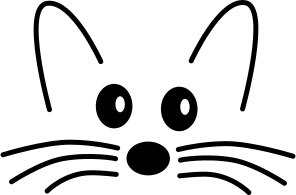
\includegraphics[width=1.4em]{squeak-logo}}}
\iftoshelse{
	\usepackage{marginnote}
		\renewcommand*{\marginfont}{\footnotesize}
	\newcommand{\vartriangleout}{\ifthenelse{\isodd{\thepage}}{\vartriangleright}{\vartriangleleft}}
	\newcommand{\dothisicon}{\fcolorbox{blue!65}{white}{\highlight{$\vartriangleout$}}}
	\newcommand{\dothis}[1]{%
		\noindent\par\noindent
		{\reversemarginpar
			\marginnote{\fcolorbox{blue!65}{white}{\highlight{$\vartriangleout$}}}}
		%\MarginLabel{do this}
		\noindent\emph{#1}
		\nopagebreak}
}{
	\newcommand{\dothisicon}{\raisebox{-.5ex}{
\includegraphics[height=1.2em]{pharo}}}
	\newcommand{\dothis}[1]{%
		\medskip
		\noindent\dothisicon
		\ifx#1\empty\else\quad\emph{#1}\fi
		\par\smallskip\nopagebreak}
}
%===> NEW VERSION <===
% NB: To use this in an individual chapter, you must set:
%\graphicspath{{figures/} {../figures/}}
% at the head of the chapter.  Don't forget the final /
%=============================================================
%:Reader hints (hint)
%
% Indicates a non-obvious consequence 
\newcommand{\hint}[1]{\vspace{1ex}\noindent\fbox{\textsc{Hint}} \emph{#1}}
%=================================================================
% graphics for Morphic handles
\newcommand{\grabHandle}{\raisebox{-0.2ex}{
\includegraphics[width=1em]{blackHandle}}}
\newcommand{\moveHandle}{\raisebox{-0.2ex}{
\includegraphics[width=1em]{moveHandle}}}
\newcommand{\debugHandle}{\raisebox{-0.2ex}{
\includegraphics[width=1em]{debugHandle}}}
%=============================================================
%:Highlighting Important stuff (doublebox)
%
% From Seaside book ...
\newsavebox{\SavedText}
\newlength{\InnerBoxRule}\setlength{\InnerBoxRule}{.75\fboxrule}
\newlength{\OuterBoxRule}\setlength{\OuterBoxRule}{1.5\fboxrule}
\newlength{\BoxSeparation}\setlength{\BoxSeparation}{1.5\fboxrule}
\addtolength{\BoxSeparation}{.5pt}
\newlength{\SaveBoxSep}\setlength{\SaveBoxSep}{2\fboxsep}
%
\newenvironment{doublebox}{\begin{lrbox}{\SavedText}
    \begin{minipage}{.75\textwidth}}
    {\end{minipage}\end{lrbox}\begin{center}
    \setlength{\fboxsep}{\BoxSeparation}\setlength{\fboxrule}{\OuterBoxRule}
    \fbox{\setlength{\fboxsep}{\SaveBoxSep}\setlength{\fboxrule}{\InnerBoxRule}%
      \fbox{\usebox{\SavedText}}}
  \end{center}}
% Use this:
\newcommand{\important}[1]{\begin{doublebox}#1\end{doublebox}}
%=============================================================
%:Section depth
\setcounter{secnumdepth}{2}
%% for this to happen start the file with
%\ifx\wholebook\relax\else
%% $Author$
% $Date$
% $Revision$

% HISTORY:
% 2006-10-31 - Oscar code macros
% ...

%=============================================================
% NB: documentclass must be set in main document.
% Allows book to be generated in multiple formats.
%=============================================================
%:Packages
\usepackage[T1]{fontenc}  %%%%%% really important to get the code directly in the text!
\usepackage{lmodern}
%\usepackage[scaled=0.85]{bookmanx} % needs another scale factor if used with \renewcommand{\sfdefault}{cmbr}
\usepackage{palatino}
\usepackage[scaled=0.85]{helvet}
\usepackage[protrusion,expansion=false]{microtype}
\usepackage{graphicx}
\usepackage{theorem}
\usepackage[english]{babel}
%%% ON: pdfsync breaks the use of p{width} for tabular columns!
%%\ifdefined\usepdfsync\usepackage{pdfsync}\fi % Requires texlive 2007
%=============================================================
%:More packages
%Stef should check which ones are used!
%\usepackage{picinpar}
%\usepackage{layout}
%\usepackage{color}
%\usepackage{enum}
%\usepackage{a4wide}
% \usepackage{fancyhdr}
\usepackage{ifthen}
\usepackage{float}
\usepackage{longtable}
\usepackage{makeidx}
\usepackage[nottoc]{tocbibind}
\usepackage{multicol}
\usepackage{booktabs}	% book-style tables
\usepackage{topcapt}	% enables \topcaption
\usepackage{multirow}
\usepackage{tabularx}
%\usepackage[bottom]{footmisc}
\usepackage{xspace}
\usepackage{alltt}
\usepackage{amssymb,textcomp}
\usepackage[usenames,dvipsnames]{color}
%\usepackage{colortbl}
\usepackage[hang]{subfigure}\makeatletter\def\p@subfigure{\thefigure\,}\makeatother
\usepackage{rotating}
\usepackage{enumitem}	% apb: allows more control over tags in enumerations
\usepackage{verbatim}     % for comment environment
\usepackage{varioref}	% for page references that work
\labelformat{footnote}{\thechapter--#1} % to distinguish citations from jurabib
\usepackage{needspace}
\usepackage{isodateo} % enable \isodate
\usepackage[newparttoc]{titlesec}
\usepackage{titletoc}
\usepackage{wrapfig}
\usepackage[
	super,
	citefull=first,
	authorformat={allreversed,and},
	titleformat={commasep,italic}
]{jurabib} % citations as footnotes
\usepackage[
	colorlinks=true,
	linkcolor=black,
	urlcolor=black,
	citecolor=black
]{hyperref}   % should come last
%=============================================================
%:PDF version
%%\pdfminorversion=3 % Set PDF to 1.3 for Lulu
%=============================================================
%:URL style
\makeatletter
\def\url@leostyle{%
  \@ifundefined{selectfont}{\def\UrlFont{\sf}}{\def\UrlFont{\sffamily}}}
\makeatother
% Now actually use the newly defined style.
\urlstyle{leo}
%=============================================================
%:Booleans
\newboolean{lulu}
\setboolean{lulu}{false}
\newcommand{\ifluluelse}[2]{\ifthenelse{\boolean{lulu}}{#1}{#2}}
%=============================================================
%:Names
\newcommand{\SUnit}{SUnit\xspace}
\newcommand{\sunit}{SUnit\xspace}
\newcommand{\xUnit}{$x$Unit\xspace}
\newcommand{\JUnit}{JUnit\xspace}
\newcommand{\st}{Smalltalk\xspace}
\newcommand{\pharo}{Pharo\xspace} % Use this, not \Pharo
%\newcommand{\sqmap}{SqueakMap\xspace}
\newcommand{\squeak}{Squeak\xspace} % use this, not \Squeak or \sq
\newcommand{\sqsrc}{SqueakSource\xspace}
\newcommand{\sbe}{\url{http://SqueakByExample.org}\xspace}
\newcommand{\pharoweb}{\url{http://pharo-project.org}\xspace}
\newcommand{\pbe}{\url{http://PharoByExample.org}\xspace}
\newcommand{\sba}{\url{http://SquareBracketAssociates.org}\xspace}
\newcommand{\bam}{\lct{Bounc\-ing\-Atoms\-Morph}\xspace}
%=============================================================
%:Markup macros for proof-reading
\usepackage[normalem]{ulem} % for \sout
\usepackage{xcolor}
\newcommand{\ra}{$\rightarrow$}
\newcommand{\ugh}[1]{\textcolor{red}{\uwave{#1}}} % please rephrase
\newcommand{\ins}[1]{\textcolor{blue}{\uline{#1}}} % please insert
\newcommand{\del}[1]{\textcolor{red}{\sout{#1}}} % please delete
\newcommand{\chg}[2]{\textcolor{red}{\sout{#1}}{\ra}\textcolor{blue}{\uline{#2}}} % please change
%=============================================================
%:Editorial comment macros
%\newcommand{\nnbb}[2]{
%    % \fbox{\bfseries\sffamily\scriptsize#1}
%    \fcolorbox{gray}{yellow}{\bfseries\sffamily\scriptsize#1}
%    {\sf\small$\blacktriangleright$\textit{#2}$\blacktriangleleft$}
%   }
\newcommand{\yellowbox}[1]{\fcolorbox{gray}{yellow}{\bfseries\sffamily\scriptsize#1}}
\newcommand{\triangles}[1]{{\sf\small$\blacktriangleright$\textit{#1}$\blacktriangleleft$}}
\newcommand{\nnbb}[2]{\yellowbox{#1} \triangles{#2}}
\newcommand{\fix}{\yellowbox{FIX!}}
\newcommand{\here}{\yellowbox{CONTINUE HERE!}}
% editor macros
\newcommand{\apl}[1]{\nnbb{Alain}{#1}} % Alain
\newcommand{\ab}[1]{\nnbb{Andrew}{#1}} % Black
\newcommand{\sd}[1]{\nnbb{St\'{e}f}{#1}} % Ducasse
\newcommand{\dc}[1]{\nnbb{DamienC}{#1}} % Ducasse
\newcommand{\md}[1]{\nnbb{Marcus}{#1}} % Denker
\newcommand{\on}[1]{\nnbb{Oscar}{#1}} % Nierstrasz
\newcommand{\damien}[1]{\nnbb{Damien}{#1}} % Pollet
\newcommand{\lr}[1]{\nnbb{Lukas}{#1}} % Renggli
\newcommand{\orla}[1]{\nnbb{Orla}{#1}} % Greevy
\newcommand{\alex}[1]{\nnbb{Alex}{#1}} % Bergel
\newcommand{\alx}[1]{\nnbb{Alex}{#1}} % Bergel
\newcommand{\dr}[1]{\nnbb{David}{#1}} % Roethlisberger
\newcommand{\ja}[1]{\nnbb{Jannik}{#1}} % Laval
\newcommand{\jr}[1]{\nnbb{Jorge}{#1}} % Ressia
\newcommand{\fp}[1]{\nnbb{Fabrizio}{#1}} % Perin
\newcommand{\michael}[1]{\nnbb{Michael}{#1}} % Davies
\newcommand{\ew}[1]{\nnbb{Erwann}{#1}} % Wernli
\newcommand{\mb}[1]{\nnbb{Martial}{#1}} % Boniou
\newcommand{\hw}[1]{\nnbb{Hernan}{#1}} % Wilkinson
%=============================================================
%:Abbreviation macros
\newcommand{\ie}{\emph{すなわち}、}
\newcommand{\eg}{\emph{例えば}、}
\newcommand{\etc}{などなど。}
%=============================================================
%:Cross reference macros
\newcommand{\charef}[1]{第~\ref{cha:#1}~章}
\newcommand{\secref}[1]{\ref{sec:#1}~節}
\newcommand{\figref}[1]{図~\ref{fig:#1}\xspace}
\newcommand{\Figref}[1]{図~\ref{fig:#1}\xspace}
\newcommand{\appref}[1]{付録~\ref{app:#1}\xspace}
\newcommand{\tabref}[1]{表~\ref{tab:#1}\xspace}
\newcommand{\faqref}[1]{FAQ~\ref{faq:#1}, p.~\pageref{faq:#1}\xspace}
% APB: I removed trailing \xspace commands from these macros because
% \xspace mostly doesn't work.  If you want a space after your
% references, type one!
% ON: xspace has always worked just fine for me!  Please leave them in.
%
\newcommand{\ruleref}[1]{\ref{rule:#1}\xspace}
%
\newcommand{\egref}[1]{example~\ref{eg:#1}\xspace}
\newcommand{\Egref}[1]{Example~\ref{eg:#1}\xspace}
%
\newcommand{\scrref}[1]{script~\ref{scr:#1}\xspace}
\newcommand{\Scrref}[1]{Script~\ref{scr:#1}\xspace}
\newcommand{\tscrref}[1]{the script~\ref{scr:#1}\xspace}
\newcommand{\Tscrref}[1]{The script~\ref{scr:#1}\xspace}
%
\newcommand{\mthref}[1]{method~\ref{mth:#1}\xspace}
\newcommand{\mthsref}[1]{methods~\ref{mth:#1}\xspace}
\newcommand{\Mthref}[1]{Method~\ref{mth:#1}\xspace}
\newcommand{\tmthref}[1]{the method~\ref{mth:#1}\xspace}
\newcommand{\Tmthref}[1]{The method~\ref{mth:#1}\xspace}
%
\newcommand{\clsref}[1]{class~\ref{cls:#1}\xspace}
\newcommand{\tclsref}[1]{the class~\ref{cls:#1}\xspace}
\newcommand{\Tclsref}[1]{The class~\ref{cls:#1}\xspace}

\newcommand{\chalabel}[1]{\label{cha:#1}}
\newcommand{\seclabel}[1]{\label{sec:#1}}
\newcommand{\figlabel}[1]{\label{fig:#1}}
\newcommand{\tablabel}[1]{\label{tab:#1}}
\newcommand{\rulelabel}[1]{\label{rule:#1}}
\newcommand{\eglabel}[1]{\label{eg:#1}}
\newcommand{\scrlabel}[1]{\label{scr:#1}}
\newcommand{\mthlabel}[1]{\label{mth:#1}}
\newcommand{\clslabel}[1]{\label{cls:#1}}
\newcommand{\faqlabel}[1]{\label{faq:#1}}
%=============================================================
%:Menu item macro
% for menu items, so we can change our minds on how to print them! (apb)
\definecolor{lightgray}{gray}{0.89}
\newcommand{\menu}[1]{{%
	\setlength{\fboxsep}{0pt}%
	\colorbox{lightgray}{{{\upshape\sffamily\strut \,#1\,}}}}}
\newcommand{\link}[1]{{%
	\fontfamily{lmr}\selectfont
 	\upshape{\sffamily \underline{#1}}}}
% For submenu items:
\newcommand{\go}{\,$\triangleright$\,}
% \newcommand{\go}{\,$\blacktriangleright$\,}
% For keyboard shortcuts:
%\newcommand{\short}[1]{\mbox{$\langle${\sc CMD}$\rangle$-#1}\xspace}
\newcommand{\short}[1]{\mbox{{\sc cmd}\hspace{0.08em}--\hspace{0.09em}#1}\xspace}
% For buttons:
\newcommand{\button}[1]{{%
	\setlength{\fboxsep}{0pt}%
	\fbox{{\upshape\sffamily\strut \,#1\,}}}}
% NB: The button macro does not work within captions -- incompatible with xcolor package :-(
\newcommand{\toolsflap}{\textit{Tools} flap\xspace}
%=============================================================
%:Mouse clicks
\newcommand{\click}{click\xspace} % RED
\newcommand{\actclick}{action-click\xspace} % YELLOW
\newcommand{\metaclick}{meta-click\xspace} % BLUE
\newcommand{\Click}{Click\xspace} % RED
\newcommand{\Actclick}{Action-click\xspace} % YELLOW
\newcommand{\Metaclick}{Meta-click\xspace} % BLUE
%=============================================================
%:ToSh macros
\newboolean{tosh}
\setboolean{tosh}{false}
\newcommand{\iftoshelse}[2]{\ifthenelse{\boolean{tosh}}{#1}{#2}}
%=============================================================
%:ToSh colors
%\newcommand{\highlightcolor}{\color{blue!65}}
%\newcommand{\boxcolor}{\color{gray!25}}
\newcommand{\highlight}[1]{\textcolor{blue!65}{#1}}
%\newcommand{\codecolor}{\color{blue!65}}
%%\setlength{\fboxrule}{2pt}
%\newcommand{\asPict}[1]{%
%	{\Large\highlight{#1}}}
%=============================================================
%:Reader cues (do this)
%
% Indicate something the reader should try out.
% \newcommand{\dothisicon}{\raisebox{-.5ex}{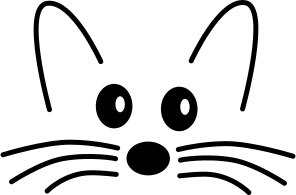
\includegraphics[width=1.4em]{squeak-logo}}}
\iftoshelse{
	\usepackage{marginnote}
		\renewcommand*{\marginfont}{\footnotesize}
	\newcommand{\vartriangleout}{\ifthenelse{\isodd{\thepage}}{\vartriangleright}{\vartriangleleft}}
	\newcommand{\dothisicon}{\fcolorbox{blue!65}{white}{\highlight{$\vartriangleout$}}}
	\newcommand{\dothis}[1]{%
		\noindent\par\noindent
		{\reversemarginpar
			\marginnote{\fcolorbox{blue!65}{white}{\highlight{$\vartriangleout$}}}}
		%\MarginLabel{do this}
		\noindent\emph{#1}
		\nopagebreak}
}{
	\newcommand{\dothisicon}{\raisebox{-.5ex}{
\includegraphics[height=1.2em]{pharo}}}
	\newcommand{\dothis}[1]{%
		\medskip
		\noindent\dothisicon
		\ifx#1\empty\else\quad\emph{#1}\fi
		\par\smallskip\nopagebreak}
}
%===> NEW VERSION <===
% NB: To use this in an individual chapter, you must set:
%\graphicspath{{figures/} {../figures/}}
% at the head of the chapter.  Don't forget the final /
%=============================================================
%:Reader hints (hint)
%
% Indicates a non-obvious consequence 
\newcommand{\hint}[1]{\vspace{1ex}\noindent\fbox{\textsc{Hint}} \emph{#1}}
%=================================================================
% graphics for Morphic handles
\newcommand{\grabHandle}{\raisebox{-0.2ex}{
\includegraphics[width=1em]{blackHandle}}}
\newcommand{\moveHandle}{\raisebox{-0.2ex}{
\includegraphics[width=1em]{moveHandle}}}
\newcommand{\debugHandle}{\raisebox{-0.2ex}{
\includegraphics[width=1em]{debugHandle}}}
%=============================================================
%:Highlighting Important stuff (doublebox)
%
% From Seaside book ...
\newsavebox{\SavedText}
\newlength{\InnerBoxRule}\setlength{\InnerBoxRule}{.75\fboxrule}
\newlength{\OuterBoxRule}\setlength{\OuterBoxRule}{1.5\fboxrule}
\newlength{\BoxSeparation}\setlength{\BoxSeparation}{1.5\fboxrule}
\addtolength{\BoxSeparation}{.5pt}
\newlength{\SaveBoxSep}\setlength{\SaveBoxSep}{2\fboxsep}
%
\newenvironment{doublebox}{\begin{lrbox}{\SavedText}
    \begin{minipage}{.75\textwidth}}
    {\end{minipage}\end{lrbox}\begin{center}
    \setlength{\fboxsep}{\BoxSeparation}\setlength{\fboxrule}{\OuterBoxRule}
    \fbox{\setlength{\fboxsep}{\SaveBoxSep}\setlength{\fboxrule}{\InnerBoxRule}%
      \fbox{\usebox{\SavedText}}}
  \end{center}}
% Use this:
\newcommand{\important}[1]{\begin{doublebox}#1\end{doublebox}}
%=============================================================
%:Section depth
\setcounter{secnumdepth}{2}
%% for this to happen start the file with
%\ifx\wholebook\relax\else
%% $Author$
% $Date$
% $Revision$

% HISTORY:
% 2006-10-31 - Oscar code macros
% ...

%=============================================================
% NB: documentclass must be set in main document.
% Allows book to be generated in multiple formats.
%=============================================================
%:Packages
\usepackage[T1]{fontenc}  %%%%%% really important to get the code directly in the text!
\usepackage{lmodern}
%\usepackage[scaled=0.85]{bookmanx} % needs another scale factor if used with \renewcommand{\sfdefault}{cmbr}
\usepackage{palatino}
\usepackage[scaled=0.85]{helvet}
\usepackage[protrusion,expansion=false]{microtype}
\usepackage{graphicx}
\usepackage{theorem}
\usepackage[english]{babel}
%%% ON: pdfsync breaks the use of p{width} for tabular columns!
%%\ifdefined\usepdfsync\usepackage{pdfsync}\fi % Requires texlive 2007
%=============================================================
%:More packages
%Stef should check which ones are used!
%\usepackage{picinpar}
%\usepackage{layout}
%\usepackage{color}
%\usepackage{enum}
%\usepackage{a4wide}
% \usepackage{fancyhdr}
\usepackage{ifthen}
\usepackage{float}
\usepackage{longtable}
\usepackage{makeidx}
\usepackage[nottoc]{tocbibind}
\usepackage{multicol}
\usepackage{booktabs}	% book-style tables
\usepackage{topcapt}	% enables \topcaption
\usepackage{multirow}
\usepackage{tabularx}
%\usepackage[bottom]{footmisc}
\usepackage{xspace}
\usepackage{alltt}
\usepackage{amssymb,textcomp}
\usepackage[usenames,dvipsnames]{color}
%\usepackage{colortbl}
\usepackage[hang]{subfigure}\makeatletter\def\p@subfigure{\thefigure\,}\makeatother
\usepackage{rotating}
\usepackage{enumitem}	% apb: allows more control over tags in enumerations
\usepackage{verbatim}     % for comment environment
\usepackage{varioref}	% for page references that work
\labelformat{footnote}{\thechapter--#1} % to distinguish citations from jurabib
\usepackage{needspace}
\usepackage{isodateo} % enable \isodate
\usepackage[newparttoc]{titlesec}
\usepackage{titletoc}
\usepackage{wrapfig}
\usepackage[
	super,
	citefull=first,
	authorformat={allreversed,and},
	titleformat={commasep,italic}
]{jurabib} % citations as footnotes
\usepackage[
	colorlinks=true,
	linkcolor=black,
	urlcolor=black,
	citecolor=black
]{hyperref}   % should come last
%=============================================================
%:PDF version
%%\pdfminorversion=3 % Set PDF to 1.3 for Lulu
%=============================================================
%:URL style
\makeatletter
\def\url@leostyle{%
  \@ifundefined{selectfont}{\def\UrlFont{\sf}}{\def\UrlFont{\sffamily}}}
\makeatother
% Now actually use the newly defined style.
\urlstyle{leo}
%=============================================================
%:Booleans
\newboolean{lulu}
\setboolean{lulu}{false}
\newcommand{\ifluluelse}[2]{\ifthenelse{\boolean{lulu}}{#1}{#2}}
%=============================================================
%:Names
\newcommand{\SUnit}{SUnit\xspace}
\newcommand{\sunit}{SUnit\xspace}
\newcommand{\xUnit}{$x$Unit\xspace}
\newcommand{\JUnit}{JUnit\xspace}
\newcommand{\st}{Smalltalk\xspace}
\newcommand{\pharo}{Pharo\xspace} % Use this, not \Pharo
%\newcommand{\sqmap}{SqueakMap\xspace}
\newcommand{\squeak}{Squeak\xspace} % use this, not \Squeak or \sq
\newcommand{\sqsrc}{SqueakSource\xspace}
\newcommand{\sbe}{\url{http://SqueakByExample.org}\xspace}
\newcommand{\pharoweb}{\url{http://pharo-project.org}\xspace}
\newcommand{\pbe}{\url{http://PharoByExample.org}\xspace}
\newcommand{\sba}{\url{http://SquareBracketAssociates.org}\xspace}
\newcommand{\bam}{\lct{Bounc\-ing\-Atoms\-Morph}\xspace}
%=============================================================
%:Markup macros for proof-reading
\usepackage[normalem]{ulem} % for \sout
\usepackage{xcolor}
\newcommand{\ra}{$\rightarrow$}
\newcommand{\ugh}[1]{\textcolor{red}{\uwave{#1}}} % please rephrase
\newcommand{\ins}[1]{\textcolor{blue}{\uline{#1}}} % please insert
\newcommand{\del}[1]{\textcolor{red}{\sout{#1}}} % please delete
\newcommand{\chg}[2]{\textcolor{red}{\sout{#1}}{\ra}\textcolor{blue}{\uline{#2}}} % please change
%=============================================================
%:Editorial comment macros
%\newcommand{\nnbb}[2]{
%    % \fbox{\bfseries\sffamily\scriptsize#1}
%    \fcolorbox{gray}{yellow}{\bfseries\sffamily\scriptsize#1}
%    {\sf\small$\blacktriangleright$\textit{#2}$\blacktriangleleft$}
%   }
\newcommand{\yellowbox}[1]{\fcolorbox{gray}{yellow}{\bfseries\sffamily\scriptsize#1}}
\newcommand{\triangles}[1]{{\sf\small$\blacktriangleright$\textit{#1}$\blacktriangleleft$}}
\newcommand{\nnbb}[2]{\yellowbox{#1} \triangles{#2}}
\newcommand{\fix}{\yellowbox{FIX!}}
\newcommand{\here}{\yellowbox{CONTINUE HERE!}}
% editor macros
\newcommand{\apl}[1]{\nnbb{Alain}{#1}} % Alain
\newcommand{\ab}[1]{\nnbb{Andrew}{#1}} % Black
\newcommand{\sd}[1]{\nnbb{St\'{e}f}{#1}} % Ducasse
\newcommand{\dc}[1]{\nnbb{DamienC}{#1}} % Ducasse
\newcommand{\md}[1]{\nnbb{Marcus}{#1}} % Denker
\newcommand{\on}[1]{\nnbb{Oscar}{#1}} % Nierstrasz
\newcommand{\damien}[1]{\nnbb{Damien}{#1}} % Pollet
\newcommand{\lr}[1]{\nnbb{Lukas}{#1}} % Renggli
\newcommand{\orla}[1]{\nnbb{Orla}{#1}} % Greevy
\newcommand{\alex}[1]{\nnbb{Alex}{#1}} % Bergel
\newcommand{\alx}[1]{\nnbb{Alex}{#1}} % Bergel
\newcommand{\dr}[1]{\nnbb{David}{#1}} % Roethlisberger
\newcommand{\ja}[1]{\nnbb{Jannik}{#1}} % Laval
\newcommand{\jr}[1]{\nnbb{Jorge}{#1}} % Ressia
\newcommand{\fp}[1]{\nnbb{Fabrizio}{#1}} % Perin
\newcommand{\michael}[1]{\nnbb{Michael}{#1}} % Davies
\newcommand{\ew}[1]{\nnbb{Erwann}{#1}} % Wernli
\newcommand{\mb}[1]{\nnbb{Martial}{#1}} % Boniou
\newcommand{\hw}[1]{\nnbb{Hernan}{#1}} % Wilkinson
%=============================================================
%:Abbreviation macros
\newcommand{\ie}{\emph{すなわち}、}
\newcommand{\eg}{\emph{例えば}、}
\newcommand{\etc}{などなど。}
%=============================================================
%:Cross reference macros
\newcommand{\charef}[1]{第~\ref{cha:#1}~章}
\newcommand{\secref}[1]{\ref{sec:#1}~節}
\newcommand{\figref}[1]{図~\ref{fig:#1}\xspace}
\newcommand{\Figref}[1]{図~\ref{fig:#1}\xspace}
\newcommand{\appref}[1]{付録~\ref{app:#1}\xspace}
\newcommand{\tabref}[1]{表~\ref{tab:#1}\xspace}
\newcommand{\faqref}[1]{FAQ~\ref{faq:#1}, p.~\pageref{faq:#1}\xspace}
% APB: I removed trailing \xspace commands from these macros because
% \xspace mostly doesn't work.  If you want a space after your
% references, type one!
% ON: xspace has always worked just fine for me!  Please leave them in.
%
\newcommand{\ruleref}[1]{\ref{rule:#1}\xspace}
%
\newcommand{\egref}[1]{example~\ref{eg:#1}\xspace}
\newcommand{\Egref}[1]{Example~\ref{eg:#1}\xspace}
%
\newcommand{\scrref}[1]{script~\ref{scr:#1}\xspace}
\newcommand{\Scrref}[1]{Script~\ref{scr:#1}\xspace}
\newcommand{\tscrref}[1]{the script~\ref{scr:#1}\xspace}
\newcommand{\Tscrref}[1]{The script~\ref{scr:#1}\xspace}
%
\newcommand{\mthref}[1]{method~\ref{mth:#1}\xspace}
\newcommand{\mthsref}[1]{methods~\ref{mth:#1}\xspace}
\newcommand{\Mthref}[1]{Method~\ref{mth:#1}\xspace}
\newcommand{\tmthref}[1]{the method~\ref{mth:#1}\xspace}
\newcommand{\Tmthref}[1]{The method~\ref{mth:#1}\xspace}
%
\newcommand{\clsref}[1]{class~\ref{cls:#1}\xspace}
\newcommand{\tclsref}[1]{the class~\ref{cls:#1}\xspace}
\newcommand{\Tclsref}[1]{The class~\ref{cls:#1}\xspace}

\newcommand{\chalabel}[1]{\label{cha:#1}}
\newcommand{\seclabel}[1]{\label{sec:#1}}
\newcommand{\figlabel}[1]{\label{fig:#1}}
\newcommand{\tablabel}[1]{\label{tab:#1}}
\newcommand{\rulelabel}[1]{\label{rule:#1}}
\newcommand{\eglabel}[1]{\label{eg:#1}}
\newcommand{\scrlabel}[1]{\label{scr:#1}}
\newcommand{\mthlabel}[1]{\label{mth:#1}}
\newcommand{\clslabel}[1]{\label{cls:#1}}
\newcommand{\faqlabel}[1]{\label{faq:#1}}
%=============================================================
%:Menu item macro
% for menu items, so we can change our minds on how to print them! (apb)
\definecolor{lightgray}{gray}{0.89}
\newcommand{\menu}[1]{{%
	\setlength{\fboxsep}{0pt}%
	\colorbox{lightgray}{{{\upshape\sffamily\strut \,#1\,}}}}}
\newcommand{\link}[1]{{%
	\fontfamily{lmr}\selectfont
 	\upshape{\sffamily \underline{#1}}}}
% For submenu items:
\newcommand{\go}{\,$\triangleright$\,}
% \newcommand{\go}{\,$\blacktriangleright$\,}
% For keyboard shortcuts:
%\newcommand{\short}[1]{\mbox{$\langle${\sc CMD}$\rangle$-#1}\xspace}
\newcommand{\short}[1]{\mbox{{\sc cmd}\hspace{0.08em}--\hspace{0.09em}#1}\xspace}
% For buttons:
\newcommand{\button}[1]{{%
	\setlength{\fboxsep}{0pt}%
	\fbox{{\upshape\sffamily\strut \,#1\,}}}}
% NB: The button macro does not work within captions -- incompatible with xcolor package :-(
\newcommand{\toolsflap}{\textit{Tools} flap\xspace}
%=============================================================
%:Mouse clicks
\newcommand{\click}{click\xspace} % RED
\newcommand{\actclick}{action-click\xspace} % YELLOW
\newcommand{\metaclick}{meta-click\xspace} % BLUE
\newcommand{\Click}{Click\xspace} % RED
\newcommand{\Actclick}{Action-click\xspace} % YELLOW
\newcommand{\Metaclick}{Meta-click\xspace} % BLUE
%=============================================================
%:ToSh macros
\newboolean{tosh}
\setboolean{tosh}{false}
\newcommand{\iftoshelse}[2]{\ifthenelse{\boolean{tosh}}{#1}{#2}}
%=============================================================
%:ToSh colors
%\newcommand{\highlightcolor}{\color{blue!65}}
%\newcommand{\boxcolor}{\color{gray!25}}
\newcommand{\highlight}[1]{\textcolor{blue!65}{#1}}
%\newcommand{\codecolor}{\color{blue!65}}
%%\setlength{\fboxrule}{2pt}
%\newcommand{\asPict}[1]{%
%	{\Large\highlight{#1}}}
%=============================================================
%:Reader cues (do this)
%
% Indicate something the reader should try out.
% \newcommand{\dothisicon}{\raisebox{-.5ex}{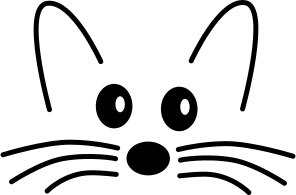
\includegraphics[width=1.4em]{squeak-logo}}}
\iftoshelse{
	\usepackage{marginnote}
		\renewcommand*{\marginfont}{\footnotesize}
	\newcommand{\vartriangleout}{\ifthenelse{\isodd{\thepage}}{\vartriangleright}{\vartriangleleft}}
	\newcommand{\dothisicon}{\fcolorbox{blue!65}{white}{\highlight{$\vartriangleout$}}}
	\newcommand{\dothis}[1]{%
		\noindent\par\noindent
		{\reversemarginpar
			\marginnote{\fcolorbox{blue!65}{white}{\highlight{$\vartriangleout$}}}}
		%\MarginLabel{do this}
		\noindent\emph{#1}
		\nopagebreak}
}{
	\newcommand{\dothisicon}{\raisebox{-.5ex}{
\includegraphics[height=1.2em]{pharo}}}
	\newcommand{\dothis}[1]{%
		\medskip
		\noindent\dothisicon
		\ifx#1\empty\else\quad\emph{#1}\fi
		\par\smallskip\nopagebreak}
}
%===> NEW VERSION <===
% NB: To use this in an individual chapter, you must set:
%\graphicspath{{figures/} {../figures/}}
% at the head of the chapter.  Don't forget the final /
%=============================================================
%:Reader hints (hint)
%
% Indicates a non-obvious consequence 
\newcommand{\hint}[1]{\vspace{1ex}\noindent\fbox{\textsc{Hint}} \emph{#1}}
%=================================================================
% graphics for Morphic handles
\newcommand{\grabHandle}{\raisebox{-0.2ex}{
\includegraphics[width=1em]{blackHandle}}}
\newcommand{\moveHandle}{\raisebox{-0.2ex}{
\includegraphics[width=1em]{moveHandle}}}
\newcommand{\debugHandle}{\raisebox{-0.2ex}{
\includegraphics[width=1em]{debugHandle}}}
%=============================================================
%:Highlighting Important stuff (doublebox)
%
% From Seaside book ...
\newsavebox{\SavedText}
\newlength{\InnerBoxRule}\setlength{\InnerBoxRule}{.75\fboxrule}
\newlength{\OuterBoxRule}\setlength{\OuterBoxRule}{1.5\fboxrule}
\newlength{\BoxSeparation}\setlength{\BoxSeparation}{1.5\fboxrule}
\addtolength{\BoxSeparation}{.5pt}
\newlength{\SaveBoxSep}\setlength{\SaveBoxSep}{2\fboxsep}
%
\newenvironment{doublebox}{\begin{lrbox}{\SavedText}
    \begin{minipage}{.75\textwidth}}
    {\end{minipage}\end{lrbox}\begin{center}
    \setlength{\fboxsep}{\BoxSeparation}\setlength{\fboxrule}{\OuterBoxRule}
    \fbox{\setlength{\fboxsep}{\SaveBoxSep}\setlength{\fboxrule}{\InnerBoxRule}%
      \fbox{\usebox{\SavedText}}}
  \end{center}}
% Use this:
\newcommand{\important}[1]{\begin{doublebox}#1\end{doublebox}}
%=============================================================
%:Section depth
\setcounter{secnumdepth}{2}
%% for this to happen start the file with
%\ifx\wholebook\relax\else
%\input{../common.tex}
%\begin{document}
%\fi
% and terminate by
% \ifx\wholebook\relax\else\end{document}\fi

\DeclareGraphicsExtensions{.pdf, .jpg, .png}
%=============================================================
%:PDF setup
\hypersetup{
%   a4paper,
%   pdfstartview=FitV,
%   colorlinks,
%   linkcolor=darkblue,
%   citecolor=darkblue,
   pdftitle={Pharo by Example},
   pdfauthor={Andrew P. Black, St\'ephane Ducasse,	Oscar Nierstrasz,
Damien Pollet},
   pdfkeywords={Smalltalk, Squeak, Object-Oriented Programming, OOP},
   pdfsubject={Computer Science}
}
%=============================================================
%:Page layout and appearance
%
% \renewcommand{\headrulewidth}{0pt}
\renewcommand{\chaptermark}[1]{\markboth{#1}{}}
\renewcommand{\sectionmark}[1]{\markright{\thesection\ #1}}
\renewpagestyle{plain}[\small\itshape]{%
	\setheadrule{0pt}%
	\sethead[][][]{}{}{}%
	\setfoot[][][]{}{}{}}
\renewpagestyle{headings}[\small\itshape]{%
	\setheadrule{0pt}%
	\setmarks{chapter}{section}%
	\sethead[\thepage][][\chaptertitle]{\sectiontitle}{}{\thepage}%
	\setfoot[][][]{}{}{}}
%=============================================================
%:Title section setup and TOC numbering depth
\setcounter{secnumdepth}{1}
\setcounter{tocdepth}{1}
\titleformat{\part}[display]{\centering}{\huge\partname\ \thepart}{1em}{\Huge\textbf}[]
\titleformat{\chapter}[display]{}{\huge\chaptertitlename\ \thechapter}{1em}{\Huge\raggedright\textbf}[]
\titlecontents{part}[3pc]{%
		\pagebreak[2]\addvspace{1em plus.4em minus.2em}%
		\leavevmode\large\bfseries}
	{\contentslabel{3pc}}{\hspace*{-3pc}}
	{}[\nopagebreak]
\titlecontents{chapter}[3pc]{%
		\pagebreak[0]\addvspace{1em plus.2em minus.2em}%
		\leavevmode\bfseries}
	{\contentslabel{3pc}}{}
	{\hfill\contentspage}[\nopagebreak]
\dottedcontents{section}[3pc]{}{3pc}{1pc}
\dottedcontents{subsection}[3pc]{}{0pc}{1pc}
% \dottedcontents{subsection}[4.5em]{}{0pt}{1pc}
% Make \cleardoublepage insert really blank pages http://www.tex.ac.uk/cgi-bin/texfaq2html?label=reallyblank
\let\origdoublepage\cleardoublepage
\newcommand{\clearemptydoublepage}{%
  \clearpage
  {\pagestyle{empty}\origdoublepage}}
\let\cleardoublepage\clearemptydoublepage % see http://www.tex.ac.uk/cgi-bin/texfaq2html?label=patch
%=============================================================
%:FAQ macros (for FAQ chapter)
\newtheorem{faq}{FAQ}
\newcommand{\answer}{\paragraph{Answer}\ }
%=============================================================
%:Listings package configuration
% \newcommand{\caret}{\makebox{\raisebox{0.4ex}{\footnotesize{$\wedge$}}}}
\newcommand{\caret}{\^\,}
\newcommand{\escape}{{\sf \textbackslash}}
\definecolor{source}{gray}{0.95}
\usepackage{listings}
\lstdefinelanguage{Smalltalk}{
%  morekeywords={self,super,true,false,nil,thisContext}, % This is overkill
  morestring=[d]',
  morecomment=[s]{"}{"},
  alsoletter={\#:},
  escapechar={!},
  literate=
    {BANG}{!}1
    {CARET}{\^}1
    {UNDERSCORE}{\_}1
    {\\st}{Smalltalk}9 % convenience -- in case \st occurs in code
    % {'}{{\textquotesingle}}1 % replaced by upquote=true in \lstset
    {_}{{$\leftarrow$}}1
    {>>>}{{\sep}}1
    {^}{{$\uparrow$}}1
    {~}{{$\sim$}}1
    {-}{{\texttt{-}}}1 %{\textminus}}1 %{-}{\hspace{-0.13em}}{-}}1  % the goal is to make - the same width as +
    % {+}{\sf+}1 %{\raisebox{0.08ex}{+}}}1      % and to raise + off the baseline to match -
    {-->}{{\quad$\longrightarrow$\quad}}3
	, % Don't forget the comma at the end!
  tabsize=4
}[keywords,comments,strings]

\lstset{language=Smalltalk,
	basicstyle=\sffamily,
	keywordstyle=\color{black}\bfseries,
	% stringstyle=\ttfamily, % Ugly! do we really want this? -- on
	mathescape=true,
	showstringspaces=false,
	keepspaces=true,
	breaklines=true,
	breakautoindent=true,
	backgroundcolor=\color{source},
	lineskip={-1pt}, % Ugly hack
	upquote=true, % straight quote; requires textcomp package
	columns=fullflexible} % no fixed width fonts
% In-line code (literal)
% Normally use this for all in-line code:
\newcommand{\ct}{\lstinline[mathescape=false,backgroundcolor=\color{white},basicstyle={\sffamily\upshape}]}
% apb 2007.8.28 added the \upshape declaration to avoid getting italicized code in \dothis{ } sections.
% In-line code (latex enabled)
% Use this only in special situations where \ct does not work
% (within section headings ...):
\newcommand{\lct}[1]{{\textsf{\textup{#1}}}}
% Use these for system categories and protocols:
\newcommand{\scat}[1]{\emph{\textsf{#1}}\xspace}
\newcommand{\pkg}[1]{\emph{\textsf{#1}}\xspace}
\newcommand{\prot}[1]{\emph{\textsf{#1}}\xspace}
% Code environments
% NB: the arg is for tests
% Only code and example environments may be tests
\lstnewenvironment{code}[1]{%
	\lstset{%
		% frame=lines,
		frame=single,
		framerule=0pt,
		mathescape=false
	}
}{}
\def\ignoredollar#1{}
%=============================================================
%:Code environments (method, script ...)
% NB: the third arg is for tests
% Only code and example environments may be tests
\lstnewenvironment{example}[3][defaultlabel]{%
	\renewcommand{\lstlistingname}{Example}%
	\lstset{
		% frame=lines,
		frame=single,
		framerule=0pt,
		mathescape=false,
		caption={\emph{#2}},
		label={eg:#1}
	}
}{}
\lstnewenvironment{script}[2][defaultlabel]{%
\renewcommand{\lstlistingname}{Script}%
	\lstset{
		% frame=lines,
		frame=single,
		framerule=0pt,
		mathescape=false,
		name={Script},
		caption={\emph{#2}},
		label={scr:#1}
	}
}{}
\lstnewenvironment{method}[2][defaultlabel]{%
	\renewcommand{\lstlistingname}{Method}%
	\lstset{
		% frame=lines,
		frame=single,
		framerule=0pt,
		mathescape=false,
		name={Method},
		caption={\emph{#2}},
		label={mth:#1}
	}
}{}
\lstnewenvironment{methods}[2][defaultlabel]{% just for multiple methods at once
	\renewcommand{\lstlistingname}{Methods}%
	\lstset{
		% frame=lines,
		frame=single,
		framerule=0pt,
		mathescape=false,
		name={Method},
		caption={\emph{#2}},
		label={mth:#1}
	}
}{}
\lstnewenvironment{numMethod}[2][defaultlabel]{%
	\renewcommand{\lstlistingname}{Method}%
	\lstset{
		numbers=left,
		numberstyle={\tiny\sffamily},
		% frame=lines,
		frame=single,
		framerule=0pt,
		mathescape=false,
		name={Method},
		caption={\emph{#2}},
		label={mth:#1}
	}
}{}
\lstnewenvironment{classdef}[2][defaultlabel]{%
	\renewcommand{\lstlistingname}{Class}%
	\lstset{
		% frame=lines,
		frame=single,
		framerule=0pt,
		mathescape=false,
		name={Class},
		caption={\emph{#2}},
		label={cls:#1}
	}
}{}
%=============================================================
%:Reserving space
% Usually need one more line than the actual lines of code
\newcommand{\needlines}[1]{\Needspace{#1\baselineskip}}
%=============================================================
%:Indexing macros
% Macros ending with "ind" generate text as well as an index entry
% Macros ending with "index" *only* generate an index entry
\newcommand{\ind}[1]{\index{#1}#1\xspace} % plain text
\newcommand{\subind}[2]{\index{#1!#2}#2\xspace} % show #2, subindex under #1
\newcommand{\emphind}[1]{\index{#1}\emph{#1}\xspace} % emph #1
\newcommand{\emphsubind}[2]{\index{#1!#2}\emph{#2}\xspace} % show emph #2, subindex inder #1
\newcommand{\scatind}[1]{\index{#1@\textsf{#1} (category)}\scat{#1}} % category
\newcommand{\pkgind}[1]{\index{#1@\textsf{#1} (package)}\pkg{#1}} % package
\newcommand{\protind}[1]{\index{#1@\textsf{#1} (protocol)}\prot{#1}} % protocol
\newcommand{\clsind}[1]{\index{#1@\textsf{#1} (class)}\ct{#1}\xspace}
% \newcommand{\clsind}[1]{\index{#1!\#@(class)}\ct{#1}\xspace} % class
\newcommand{\clsindplural}[1]{\index{#1!\#@(class)}\ct{#1}s\xspace} % class
\newcommand{\cvind}[1]{\index{#1@\textsf{#1} (class variable)}\ct{#1}\xspace} % class var
\newcommand{\glbind}[1]{\index{#1@\textsf{#1} (global)}\ct{#1}\xspace} % global
\newcommand{\patind}[1]{\index{#1@#1 (pattern)}\ct{#1}\xspace} % pattern
\newcommand{\pvind}[1]{\index{#1@\textsf{#1} (pseudo variable)}\ct{#1}\xspace} % pseudo var
\newcommand{\clsmthind}[2]{\index{#1!#2@\ct{#2}}\ct{#1>>>#2}\xspace} % class + method name
\newcommand{\mthind}[2]{\index{#1!#2@\ct{#2}}\ct{#2}\xspace} % show method name only
\newcommand{\lmthind}[2]{\index{#1!#2@\ct{#2}}\lct{#2}\xspace} % show method name only
\newcommand{\cmind}[2]{\index{#1!#2@\ct{#2}}\ct{#1>>>#2}\xspace} % show class>>method
\newcommand{\lcmind}[2]{\index{#1!#2@\ct{#2}}\lct{#1>>>#2}\xspace} % show class>>method
\newcommand{\toolsflapind}{\index{Tools flap}\toolsflap} % index tools flap
% The following only generate an index entry:
% \newcommand{\clsindex}[1]{\index{#1@\textsf{#1} (class)}}
\newcommand{\clsindex}[1]{\index{#1!\#@(class)}} % class
\newcommand{\mthindex}[2]{\index{#1!#2@\ct{#2}}} % method
\newcommand{\cmindex}[2]{\index{#1!#2@\ct{#2}}} % class>>method
\newcommand{\cvindex}[1]{\index{#1@\textsf{#1} (class variable)}} % class var
\newcommand{\glbindex}[1]{\index{#1@\textsf{#1} (global)}}% global
\newcommand{\pvindex}[1]{\index{#1@\textsf{#1} (pseudo variable)}}% pseudo var
\newcommand{\seeindex}[2]{\index{#1|see{#2}}} % #1, see #2
\newcommand{\scatindex}[1]{\index{#1@\textsf{#1} (category)}} % category
\newcommand{\pkgindex}[1]{\index{#1@\textsf{#1} (package)}} % package
\newcommand{\protindex}[1]{\index{#1@\textsf{#1} (protocol)}} % protocol
% How can we have the main entry page numbers in bold yet not break the hyperlink?
\newcommand{\boldidx}[1]{{\bf #1}} % breaks hyperlink
%\newcommand{\indmain}[1]{\index{#1|boldidx}#1\xspace} % plain text, main entry
%\newcommand{\emphsubindmain}[2]{\index{#1!#2|boldidx}\emph{#2}\xspace} % subindex, main entry
%\newcommand{\subindmain}[2]{\index{#1!#2|boldidx}#2\xspace} % subindex, main entry
%\newcommand{\clsindmain}[1]{\index{#1@\textsf{#1} (class)|boldidx}\ct{#1}\xspace}
%\newcommand{\clsindmain}[1]{\index{#1!\#@(class)|boldidx}\ct{#1}\xspace} % class main
%\newcommand{\indexmain}[1]{\index{#1|boldidx}} % main index entry only
\newcommand{\indmain}[1]{\index{#1}#1\xspace} % The main index entry for this item
\newcommand{\emphsubindmain}[2]{\index{#1!#2}\emph{#2}\xspace} % subindex, main entry
\newcommand{\subindmain}[2]{\index{#1!#2}#2\xspace} % subindex, main entry
%\newcommand{\clsindmain}[1]{\index{#1@\textsf{#1} (class)}\ct{#1}\xspace}
\newcommand{\clsindmain}[1]{\index{#1!\#@(class)}\ct{#1}\xspace} % class main
\newcommand{\clsindexmain}[1]{\index{#1!\#@(class)}} % class main index only
\newcommand{\indexmain}[1]{\index{#1}} 
%=============================================================
%:Code macros
% some constants
\newcommand{\codesize}{\small}
\newcommand{\codefont}{\sffamily}
%\newcommand{\cat}[1]{\textit{In category #1}}%%To remove later
\newlength{\scriptindent}
\setlength{\scriptindent}{.3cm}
%% Method presentation constants
\newlength{\methodindent}
\newlength{\methodwordlength}
\newlength{\aftermethod}
\setlength{\methodindent}{0.2cm}
\settowidth{\methodwordlength}{\ M\'ethode\ }
%=============================================================
%:Smalltalk macros
%\newcommand{\sep}{{$\gg$}}
\newcommand{\sep}{\mbox{>>}}
\newcommand{\self}{\lct{self}\xspace}
\newcommand{\super}{\lct{super}\xspace}
\newcommand{\nil}{\lct{nil}\xspace}
%=============================================================
% be less conservative about float placement
% these commands are from http://www.tex.ac.uk/cgi-bin/texfaq2html?label=floats
\renewcommand{\topfraction}{.9}
\renewcommand{\bottomfraction}{.9}
\renewcommand{\textfraction}{.1}
\renewcommand{\floatpagefraction}{.85}
\renewcommand{\dbltopfraction}{.66}
\renewcommand{\dblfloatpagefraction}{.85}
\setcounter{topnumber}{9}
\setcounter{bottomnumber}{9}
\setcounter{totalnumber}{20}
\setcounter{dbltopnumber}{9}
%=============================================================
% Give information from each chapter's author
\newcommand{\contact}[2]{\textbf{#1} \textsf{(#2)}}

\newcommand{\chapterauthor}[1]{\emph{with the participation of:\\#1}\\}

\newcommand{\authornoury}{\contact{Noury Bouraqadi}{bouraqadi@gmail.com}}
\newcommand{\authordamienc}{\contact{Damien Cassou}{damien.cassou@gmail.com}}
\newcommand{\authoroscar}{\contact{Oscar Nierstrasz}{oscar.nierstrasz@acm.org}}
\newcommand{\authorsteph}{\contact{St\'ephane Ducasse}{stephane.ducasse@inria.fr}}
\newcommand{\authoralex}{\contact{Alexandre Bergel}{alexandre@bergel.eu}}
\newcommand{\authorolivier}{\contact{Olivier Auverlot}{olivier.auverlot@inria.fr}}
\newcommand{\authornicolas}{\contact{Nicolas Cellier}{ncellier@ifrance.com}}
\newcommand{\authormarcus}{\contact{Marcus Denker}{marcus.denker@inria.fr}}
\newcommand{\authoralain}{\contact{Alain Plantec}{alain.plantec@univ-brest.fr}}
\newcommand{\authordale}{\contact{Dale Henrichs}{dale.henrichs@gemstone.com}}
\newcommand{\authormariano}{\contact{Mariano Martinez Peck}{marianopeck@gmail.com}}
\newcommand{\authorsven}{\contact{Sven Van Caekenberghe}{sven@beta9.be}}

%=============================================================
% apb doesn't like paragraphs to run in to each other without a break
\parskip 1ex
%=============================================================
%:Stuff to check, merge or deprecate
%\setlength{\marginparsep}{2mm}
%\renewcommand{\baselinestretch}{1.1}
%=============================================================

%\begin{document}
%\fi
% and terminate by
% \ifx\wholebook\relax\else\end{document}\fi

\DeclareGraphicsExtensions{.pdf, .jpg, .png}
%=============================================================
%:PDF setup
\hypersetup{
%   a4paper,
%   pdfstartview=FitV,
%   colorlinks,
%   linkcolor=darkblue,
%   citecolor=darkblue,
   pdftitle={Pharo by Example},
   pdfauthor={Andrew P. Black, St\'ephane Ducasse,	Oscar Nierstrasz,
Damien Pollet},
   pdfkeywords={Smalltalk, Squeak, Object-Oriented Programming, OOP},
   pdfsubject={Computer Science}
}
%=============================================================
%:Page layout and appearance
%
% \renewcommand{\headrulewidth}{0pt}
\renewcommand{\chaptermark}[1]{\markboth{#1}{}}
\renewcommand{\sectionmark}[1]{\markright{\thesection\ #1}}
\renewpagestyle{plain}[\small\itshape]{%
	\setheadrule{0pt}%
	\sethead[][][]{}{}{}%
	\setfoot[][][]{}{}{}}
\renewpagestyle{headings}[\small\itshape]{%
	\setheadrule{0pt}%
	\setmarks{chapter}{section}%
	\sethead[\thepage][][\chaptertitle]{\sectiontitle}{}{\thepage}%
	\setfoot[][][]{}{}{}}
%=============================================================
%:Title section setup and TOC numbering depth
\setcounter{secnumdepth}{1}
\setcounter{tocdepth}{1}
\titleformat{\part}[display]{\centering}{\huge\partname\ \thepart}{1em}{\Huge\textbf}[]
\titleformat{\chapter}[display]{}{\huge\chaptertitlename\ \thechapter}{1em}{\Huge\raggedright\textbf}[]
\titlecontents{part}[3pc]{%
		\pagebreak[2]\addvspace{1em plus.4em minus.2em}%
		\leavevmode\large\bfseries}
	{\contentslabel{3pc}}{\hspace*{-3pc}}
	{}[\nopagebreak]
\titlecontents{chapter}[3pc]{%
		\pagebreak[0]\addvspace{1em plus.2em minus.2em}%
		\leavevmode\bfseries}
	{\contentslabel{3pc}}{}
	{\hfill\contentspage}[\nopagebreak]
\dottedcontents{section}[3pc]{}{3pc}{1pc}
\dottedcontents{subsection}[3pc]{}{0pc}{1pc}
% \dottedcontents{subsection}[4.5em]{}{0pt}{1pc}
% Make \cleardoublepage insert really blank pages http://www.tex.ac.uk/cgi-bin/texfaq2html?label=reallyblank
\let\origdoublepage\cleardoublepage
\newcommand{\clearemptydoublepage}{%
  \clearpage
  {\pagestyle{empty}\origdoublepage}}
\let\cleardoublepage\clearemptydoublepage % see http://www.tex.ac.uk/cgi-bin/texfaq2html?label=patch
%=============================================================
%:FAQ macros (for FAQ chapter)
\newtheorem{faq}{FAQ}
\newcommand{\answer}{\paragraph{Answer}\ }
%=============================================================
%:Listings package configuration
% \newcommand{\caret}{\makebox{\raisebox{0.4ex}{\footnotesize{$\wedge$}}}}
\newcommand{\caret}{\^\,}
\newcommand{\escape}{{\sf \textbackslash}}
\definecolor{source}{gray}{0.95}
\usepackage{listings}
\lstdefinelanguage{Smalltalk}{
%  morekeywords={self,super,true,false,nil,thisContext}, % This is overkill
  morestring=[d]',
  morecomment=[s]{"}{"},
  alsoletter={\#:},
  escapechar={!},
  literate=
    {BANG}{!}1
    {CARET}{\^}1
    {UNDERSCORE}{\_}1
    {\\st}{Smalltalk}9 % convenience -- in case \st occurs in code
    % {'}{{\textquotesingle}}1 % replaced by upquote=true in \lstset
    {_}{{$\leftarrow$}}1
    {>>>}{{\sep}}1
    {^}{{$\uparrow$}}1
    {~}{{$\sim$}}1
    {-}{{\texttt{-}}}1 %{\textminus}}1 %{-}{\hspace{-0.13em}}{-}}1  % the goal is to make - the same width as +
    % {+}{\sf+}1 %{\raisebox{0.08ex}{+}}}1      % and to raise + off the baseline to match -
    {-->}{{\quad$\longrightarrow$\quad}}3
	, % Don't forget the comma at the end!
  tabsize=4
}[keywords,comments,strings]

\lstset{language=Smalltalk,
	basicstyle=\sffamily,
	keywordstyle=\color{black}\bfseries,
	% stringstyle=\ttfamily, % Ugly! do we really want this? -- on
	mathescape=true,
	showstringspaces=false,
	keepspaces=true,
	breaklines=true,
	breakautoindent=true,
	backgroundcolor=\color{source},
	lineskip={-1pt}, % Ugly hack
	upquote=true, % straight quote; requires textcomp package
	columns=fullflexible} % no fixed width fonts
% In-line code (literal)
% Normally use this for all in-line code:
\newcommand{\ct}{\lstinline[mathescape=false,backgroundcolor=\color{white},basicstyle={\sffamily\upshape}]}
% apb 2007.8.28 added the \upshape declaration to avoid getting italicized code in \dothis{ } sections.
% In-line code (latex enabled)
% Use this only in special situations where \ct does not work
% (within section headings ...):
\newcommand{\lct}[1]{{\textsf{\textup{#1}}}}
% Use these for system categories and protocols:
\newcommand{\scat}[1]{\emph{\textsf{#1}}\xspace}
\newcommand{\pkg}[1]{\emph{\textsf{#1}}\xspace}
\newcommand{\prot}[1]{\emph{\textsf{#1}}\xspace}
% Code environments
% NB: the arg is for tests
% Only code and example environments may be tests
\lstnewenvironment{code}[1]{%
	\lstset{%
		% frame=lines,
		frame=single,
		framerule=0pt,
		mathescape=false
	}
}{}
\def\ignoredollar#1{}
%=============================================================
%:Code environments (method, script ...)
% NB: the third arg is for tests
% Only code and example environments may be tests
\lstnewenvironment{example}[3][defaultlabel]{%
	\renewcommand{\lstlistingname}{Example}%
	\lstset{
		% frame=lines,
		frame=single,
		framerule=0pt,
		mathescape=false,
		caption={\emph{#2}},
		label={eg:#1}
	}
}{}
\lstnewenvironment{script}[2][defaultlabel]{%
\renewcommand{\lstlistingname}{Script}%
	\lstset{
		% frame=lines,
		frame=single,
		framerule=0pt,
		mathescape=false,
		name={Script},
		caption={\emph{#2}},
		label={scr:#1}
	}
}{}
\lstnewenvironment{method}[2][defaultlabel]{%
	\renewcommand{\lstlistingname}{Method}%
	\lstset{
		% frame=lines,
		frame=single,
		framerule=0pt,
		mathescape=false,
		name={Method},
		caption={\emph{#2}},
		label={mth:#1}
	}
}{}
\lstnewenvironment{methods}[2][defaultlabel]{% just for multiple methods at once
	\renewcommand{\lstlistingname}{Methods}%
	\lstset{
		% frame=lines,
		frame=single,
		framerule=0pt,
		mathescape=false,
		name={Method},
		caption={\emph{#2}},
		label={mth:#1}
	}
}{}
\lstnewenvironment{numMethod}[2][defaultlabel]{%
	\renewcommand{\lstlistingname}{Method}%
	\lstset{
		numbers=left,
		numberstyle={\tiny\sffamily},
		% frame=lines,
		frame=single,
		framerule=0pt,
		mathescape=false,
		name={Method},
		caption={\emph{#2}},
		label={mth:#1}
	}
}{}
\lstnewenvironment{classdef}[2][defaultlabel]{%
	\renewcommand{\lstlistingname}{Class}%
	\lstset{
		% frame=lines,
		frame=single,
		framerule=0pt,
		mathescape=false,
		name={Class},
		caption={\emph{#2}},
		label={cls:#1}
	}
}{}
%=============================================================
%:Reserving space
% Usually need one more line than the actual lines of code
\newcommand{\needlines}[1]{\Needspace{#1\baselineskip}}
%=============================================================
%:Indexing macros
% Macros ending with "ind" generate text as well as an index entry
% Macros ending with "index" *only* generate an index entry
\newcommand{\ind}[1]{\index{#1}#1\xspace} % plain text
\newcommand{\subind}[2]{\index{#1!#2}#2\xspace} % show #2, subindex under #1
\newcommand{\emphind}[1]{\index{#1}\emph{#1}\xspace} % emph #1
\newcommand{\emphsubind}[2]{\index{#1!#2}\emph{#2}\xspace} % show emph #2, subindex inder #1
\newcommand{\scatind}[1]{\index{#1@\textsf{#1} (category)}\scat{#1}} % category
\newcommand{\pkgind}[1]{\index{#1@\textsf{#1} (package)}\pkg{#1}} % package
\newcommand{\protind}[1]{\index{#1@\textsf{#1} (protocol)}\prot{#1}} % protocol
\newcommand{\clsind}[1]{\index{#1@\textsf{#1} (class)}\ct{#1}\xspace}
% \newcommand{\clsind}[1]{\index{#1!\#@(class)}\ct{#1}\xspace} % class
\newcommand{\clsindplural}[1]{\index{#1!\#@(class)}\ct{#1}s\xspace} % class
\newcommand{\cvind}[1]{\index{#1@\textsf{#1} (class variable)}\ct{#1}\xspace} % class var
\newcommand{\glbind}[1]{\index{#1@\textsf{#1} (global)}\ct{#1}\xspace} % global
\newcommand{\patind}[1]{\index{#1@#1 (pattern)}\ct{#1}\xspace} % pattern
\newcommand{\pvind}[1]{\index{#1@\textsf{#1} (pseudo variable)}\ct{#1}\xspace} % pseudo var
\newcommand{\clsmthind}[2]{\index{#1!#2@\ct{#2}}\ct{#1>>>#2}\xspace} % class + method name
\newcommand{\mthind}[2]{\index{#1!#2@\ct{#2}}\ct{#2}\xspace} % show method name only
\newcommand{\lmthind}[2]{\index{#1!#2@\ct{#2}}\lct{#2}\xspace} % show method name only
\newcommand{\cmind}[2]{\index{#1!#2@\ct{#2}}\ct{#1>>>#2}\xspace} % show class>>method
\newcommand{\lcmind}[2]{\index{#1!#2@\ct{#2}}\lct{#1>>>#2}\xspace} % show class>>method
\newcommand{\toolsflapind}{\index{Tools flap}\toolsflap} % index tools flap
% The following only generate an index entry:
% \newcommand{\clsindex}[1]{\index{#1@\textsf{#1} (class)}}
\newcommand{\clsindex}[1]{\index{#1!\#@(class)}} % class
\newcommand{\mthindex}[2]{\index{#1!#2@\ct{#2}}} % method
\newcommand{\cmindex}[2]{\index{#1!#2@\ct{#2}}} % class>>method
\newcommand{\cvindex}[1]{\index{#1@\textsf{#1} (class variable)}} % class var
\newcommand{\glbindex}[1]{\index{#1@\textsf{#1} (global)}}% global
\newcommand{\pvindex}[1]{\index{#1@\textsf{#1} (pseudo variable)}}% pseudo var
\newcommand{\seeindex}[2]{\index{#1|see{#2}}} % #1, see #2
\newcommand{\scatindex}[1]{\index{#1@\textsf{#1} (category)}} % category
\newcommand{\pkgindex}[1]{\index{#1@\textsf{#1} (package)}} % package
\newcommand{\protindex}[1]{\index{#1@\textsf{#1} (protocol)}} % protocol
% How can we have the main entry page numbers in bold yet not break the hyperlink?
\newcommand{\boldidx}[1]{{\bf #1}} % breaks hyperlink
%\newcommand{\indmain}[1]{\index{#1|boldidx}#1\xspace} % plain text, main entry
%\newcommand{\emphsubindmain}[2]{\index{#1!#2|boldidx}\emph{#2}\xspace} % subindex, main entry
%\newcommand{\subindmain}[2]{\index{#1!#2|boldidx}#2\xspace} % subindex, main entry
%\newcommand{\clsindmain}[1]{\index{#1@\textsf{#1} (class)|boldidx}\ct{#1}\xspace}
%\newcommand{\clsindmain}[1]{\index{#1!\#@(class)|boldidx}\ct{#1}\xspace} % class main
%\newcommand{\indexmain}[1]{\index{#1|boldidx}} % main index entry only
\newcommand{\indmain}[1]{\index{#1}#1\xspace} % The main index entry for this item
\newcommand{\emphsubindmain}[2]{\index{#1!#2}\emph{#2}\xspace} % subindex, main entry
\newcommand{\subindmain}[2]{\index{#1!#2}#2\xspace} % subindex, main entry
%\newcommand{\clsindmain}[1]{\index{#1@\textsf{#1} (class)}\ct{#1}\xspace}
\newcommand{\clsindmain}[1]{\index{#1!\#@(class)}\ct{#1}\xspace} % class main
\newcommand{\clsindexmain}[1]{\index{#1!\#@(class)}} % class main index only
\newcommand{\indexmain}[1]{\index{#1}} 
%=============================================================
%:Code macros
% some constants
\newcommand{\codesize}{\small}
\newcommand{\codefont}{\sffamily}
%\newcommand{\cat}[1]{\textit{In category #1}}%%To remove later
\newlength{\scriptindent}
\setlength{\scriptindent}{.3cm}
%% Method presentation constants
\newlength{\methodindent}
\newlength{\methodwordlength}
\newlength{\aftermethod}
\setlength{\methodindent}{0.2cm}
\settowidth{\methodwordlength}{\ M\'ethode\ }
%=============================================================
%:Smalltalk macros
%\newcommand{\sep}{{$\gg$}}
\newcommand{\sep}{\mbox{>>}}
\newcommand{\self}{\lct{self}\xspace}
\newcommand{\super}{\lct{super}\xspace}
\newcommand{\nil}{\lct{nil}\xspace}
%=============================================================
% be less conservative about float placement
% these commands are from http://www.tex.ac.uk/cgi-bin/texfaq2html?label=floats
\renewcommand{\topfraction}{.9}
\renewcommand{\bottomfraction}{.9}
\renewcommand{\textfraction}{.1}
\renewcommand{\floatpagefraction}{.85}
\renewcommand{\dbltopfraction}{.66}
\renewcommand{\dblfloatpagefraction}{.85}
\setcounter{topnumber}{9}
\setcounter{bottomnumber}{9}
\setcounter{totalnumber}{20}
\setcounter{dbltopnumber}{9}
%=============================================================
% Give information from each chapter's author
\newcommand{\contact}[2]{\textbf{#1} \textsf{(#2)}}

\newcommand{\chapterauthor}[1]{\emph{with the participation of:\\#1}\\}

\newcommand{\authornoury}{\contact{Noury Bouraqadi}{bouraqadi@gmail.com}}
\newcommand{\authordamienc}{\contact{Damien Cassou}{damien.cassou@gmail.com}}
\newcommand{\authoroscar}{\contact{Oscar Nierstrasz}{oscar.nierstrasz@acm.org}}
\newcommand{\authorsteph}{\contact{St\'ephane Ducasse}{stephane.ducasse@inria.fr}}
\newcommand{\authoralex}{\contact{Alexandre Bergel}{alexandre@bergel.eu}}
\newcommand{\authorolivier}{\contact{Olivier Auverlot}{olivier.auverlot@inria.fr}}
\newcommand{\authornicolas}{\contact{Nicolas Cellier}{ncellier@ifrance.com}}
\newcommand{\authormarcus}{\contact{Marcus Denker}{marcus.denker@inria.fr}}
\newcommand{\authoralain}{\contact{Alain Plantec}{alain.plantec@univ-brest.fr}}
\newcommand{\authordale}{\contact{Dale Henrichs}{dale.henrichs@gemstone.com}}
\newcommand{\authormariano}{\contact{Mariano Martinez Peck}{marianopeck@gmail.com}}
\newcommand{\authorsven}{\contact{Sven Van Caekenberghe}{sven@beta9.be}}

%=============================================================
% apb doesn't like paragraphs to run in to each other without a break
\parskip 1ex
%=============================================================
%:Stuff to check, merge or deprecate
%\setlength{\marginparsep}{2mm}
%\renewcommand{\baselinestretch}{1.1}
%=============================================================

%\begin{document}
%\fi
% and terminate by
% \ifx\wholebook\relax\else\end{document}\fi

\DeclareGraphicsExtensions{.pdf, .jpg, .png}
%=============================================================
%:PDF setup
\hypersetup{
%   a4paper,
%   pdfstartview=FitV,
%   colorlinks,
%   linkcolor=darkblue,
%   citecolor=darkblue,
   pdftitle={Pharo by Example},
   pdfauthor={Andrew P. Black, St\'ephane Ducasse,	Oscar Nierstrasz,
Damien Pollet},
   pdfkeywords={Smalltalk, Squeak, Object-Oriented Programming, OOP},
   pdfsubject={Computer Science}
}
%=============================================================
%:Page layout and appearance
%
% \renewcommand{\headrulewidth}{0pt}
\renewcommand{\chaptermark}[1]{\markboth{#1}{}}
\renewcommand{\sectionmark}[1]{\markright{\thesection\ #1}}
\renewpagestyle{plain}[\small\itshape]{%
	\setheadrule{0pt}%
	\sethead[][][]{}{}{}%
	\setfoot[][][]{}{}{}}
\renewpagestyle{headings}[\small\itshape]{%
	\setheadrule{0pt}%
	\setmarks{chapter}{section}%
	\sethead[\thepage][][\chaptertitle]{\sectiontitle}{}{\thepage}%
	\setfoot[][][]{}{}{}}
%=============================================================
%:Title section setup and TOC numbering depth
\setcounter{secnumdepth}{1}
\setcounter{tocdepth}{1}
\titleformat{\part}[display]{\centering}{\huge\partname\ \thepart}{1em}{\Huge\textbf}[]
\titleformat{\chapter}[display]{}{\huge\chaptertitlename\ \thechapter}{1em}{\Huge\raggedright\textbf}[]
\titlecontents{part}[3pc]{%
		\pagebreak[2]\addvspace{1em plus.4em minus.2em}%
		\leavevmode\large\bfseries}
	{\contentslabel{3pc}}{\hspace*{-3pc}}
	{}[\nopagebreak]
\titlecontents{chapter}[3pc]{%
		\pagebreak[0]\addvspace{1em plus.2em minus.2em}%
		\leavevmode\bfseries}
	{\contentslabel{3pc}}{}
	{\hfill\contentspage}[\nopagebreak]
\dottedcontents{section}[3pc]{}{3pc}{1pc}
\dottedcontents{subsection}[3pc]{}{0pc}{1pc}
% \dottedcontents{subsection}[4.5em]{}{0pt}{1pc}
% Make \cleardoublepage insert really blank pages http://www.tex.ac.uk/cgi-bin/texfaq2html?label=reallyblank
\let\origdoublepage\cleardoublepage
\newcommand{\clearemptydoublepage}{%
  \clearpage
  {\pagestyle{empty}\origdoublepage}}
\let\cleardoublepage\clearemptydoublepage % see http://www.tex.ac.uk/cgi-bin/texfaq2html?label=patch
%=============================================================
%:FAQ macros (for FAQ chapter)
\newtheorem{faq}{FAQ}
\newcommand{\answer}{\paragraph{Answer}\ }
%=============================================================
%:Listings package configuration
% \newcommand{\caret}{\makebox{\raisebox{0.4ex}{\footnotesize{$\wedge$}}}}
\newcommand{\caret}{\^\,}
\newcommand{\escape}{{\sf \textbackslash}}
\definecolor{source}{gray}{0.95}
\usepackage{listings}
\lstdefinelanguage{Smalltalk}{
%  morekeywords={self,super,true,false,nil,thisContext}, % This is overkill
  morestring=[d]',
  morecomment=[s]{"}{"},
  alsoletter={\#:},
  escapechar={!},
  literate=
    {BANG}{!}1
    {CARET}{\^}1
    {UNDERSCORE}{\_}1
    {\\st}{Smalltalk}9 % convenience -- in case \st occurs in code
    % {'}{{\textquotesingle}}1 % replaced by upquote=true in \lstset
    {_}{{$\leftarrow$}}1
    {>>>}{{\sep}}1
    {^}{{$\uparrow$}}1
    {~}{{$\sim$}}1
    {-}{{\texttt{-}}}1 %{\textminus}}1 %{-}{\hspace{-0.13em}}{-}}1  % the goal is to make - the same width as +
    % {+}{\sf+}1 %{\raisebox{0.08ex}{+}}}1      % and to raise + off the baseline to match -
    {-->}{{\quad$\longrightarrow$\quad}}3
	, % Don't forget the comma at the end!
  tabsize=4
}[keywords,comments,strings]

\lstset{language=Smalltalk,
	basicstyle=\sffamily,
	keywordstyle=\color{black}\bfseries,
	% stringstyle=\ttfamily, % Ugly! do we really want this? -- on
	mathescape=true,
	showstringspaces=false,
	keepspaces=true,
	breaklines=true,
	breakautoindent=true,
	backgroundcolor=\color{source},
	lineskip={-1pt}, % Ugly hack
	upquote=true, % straight quote; requires textcomp package
	columns=fullflexible} % no fixed width fonts
% In-line code (literal)
% Normally use this for all in-line code:
\newcommand{\ct}{\lstinline[mathescape=false,backgroundcolor=\color{white},basicstyle={\sffamily\upshape}]}
% apb 2007.8.28 added the \upshape declaration to avoid getting italicized code in \dothis{ } sections.
% In-line code (latex enabled)
% Use this only in special situations where \ct does not work
% (within section headings ...):
\newcommand{\lct}[1]{{\textsf{\textup{#1}}}}
% Use these for system categories and protocols:
\newcommand{\scat}[1]{\emph{\textsf{#1}}\xspace}
\newcommand{\pkg}[1]{\emph{\textsf{#1}}\xspace}
\newcommand{\prot}[1]{\emph{\textsf{#1}}\xspace}
% Code environments
% NB: the arg is for tests
% Only code and example environments may be tests
\lstnewenvironment{code}[1]{%
	\lstset{%
		% frame=lines,
		frame=single,
		framerule=0pt,
		mathescape=false
	}
}{}
\def\ignoredollar#1{}
%=============================================================
%:Code environments (method, script ...)
% NB: the third arg is for tests
% Only code and example environments may be tests
\lstnewenvironment{example}[3][defaultlabel]{%
	\renewcommand{\lstlistingname}{Example}%
	\lstset{
		% frame=lines,
		frame=single,
		framerule=0pt,
		mathescape=false,
		caption={\emph{#2}},
		label={eg:#1}
	}
}{}
\lstnewenvironment{script}[2][defaultlabel]{%
\renewcommand{\lstlistingname}{Script}%
	\lstset{
		% frame=lines,
		frame=single,
		framerule=0pt,
		mathescape=false,
		name={Script},
		caption={\emph{#2}},
		label={scr:#1}
	}
}{}
\lstnewenvironment{method}[2][defaultlabel]{%
	\renewcommand{\lstlistingname}{Method}%
	\lstset{
		% frame=lines,
		frame=single,
		framerule=0pt,
		mathescape=false,
		name={Method},
		caption={\emph{#2}},
		label={mth:#1}
	}
}{}
\lstnewenvironment{methods}[2][defaultlabel]{% just for multiple methods at once
	\renewcommand{\lstlistingname}{Methods}%
	\lstset{
		% frame=lines,
		frame=single,
		framerule=0pt,
		mathescape=false,
		name={Method},
		caption={\emph{#2}},
		label={mth:#1}
	}
}{}
\lstnewenvironment{numMethod}[2][defaultlabel]{%
	\renewcommand{\lstlistingname}{Method}%
	\lstset{
		numbers=left,
		numberstyle={\tiny\sffamily},
		% frame=lines,
		frame=single,
		framerule=0pt,
		mathescape=false,
		name={Method},
		caption={\emph{#2}},
		label={mth:#1}
	}
}{}
\lstnewenvironment{classdef}[2][defaultlabel]{%
	\renewcommand{\lstlistingname}{Class}%
	\lstset{
		% frame=lines,
		frame=single,
		framerule=0pt,
		mathescape=false,
		name={Class},
		caption={\emph{#2}},
		label={cls:#1}
	}
}{}
%=============================================================
%:Reserving space
% Usually need one more line than the actual lines of code
\newcommand{\needlines}[1]{\Needspace{#1\baselineskip}}
%=============================================================
%:Indexing macros
% Macros ending with "ind" generate text as well as an index entry
% Macros ending with "index" *only* generate an index entry
\newcommand{\ind}[1]{\index{#1}#1\xspace} % plain text
\newcommand{\subind}[2]{\index{#1!#2}#2\xspace} % show #2, subindex under #1
\newcommand{\emphind}[1]{\index{#1}\emph{#1}\xspace} % emph #1
\newcommand{\emphsubind}[2]{\index{#1!#2}\emph{#2}\xspace} % show emph #2, subindex inder #1
\newcommand{\scatind}[1]{\index{#1@\textsf{#1} (category)}\scat{#1}} % category
\newcommand{\pkgind}[1]{\index{#1@\textsf{#1} (package)}\pkg{#1}} % package
\newcommand{\protind}[1]{\index{#1@\textsf{#1} (protocol)}\prot{#1}} % protocol
\newcommand{\clsind}[1]{\index{#1@\textsf{#1} (class)}\ct{#1}\xspace}
% \newcommand{\clsind}[1]{\index{#1!\#@(class)}\ct{#1}\xspace} % class
\newcommand{\clsindplural}[1]{\index{#1!\#@(class)}\ct{#1}s\xspace} % class
\newcommand{\cvind}[1]{\index{#1@\textsf{#1} (class variable)}\ct{#1}\xspace} % class var
\newcommand{\glbind}[1]{\index{#1@\textsf{#1} (global)}\ct{#1}\xspace} % global
\newcommand{\patind}[1]{\index{#1@#1 (pattern)}\ct{#1}\xspace} % pattern
\newcommand{\pvind}[1]{\index{#1@\textsf{#1} (pseudo variable)}\ct{#1}\xspace} % pseudo var
\newcommand{\clsmthind}[2]{\index{#1!#2@\ct{#2}}\ct{#1>>>#2}\xspace} % class + method name
\newcommand{\mthind}[2]{\index{#1!#2@\ct{#2}}\ct{#2}\xspace} % show method name only
\newcommand{\lmthind}[2]{\index{#1!#2@\ct{#2}}\lct{#2}\xspace} % show method name only
\newcommand{\cmind}[2]{\index{#1!#2@\ct{#2}}\ct{#1>>>#2}\xspace} % show class>>method
\newcommand{\lcmind}[2]{\index{#1!#2@\ct{#2}}\lct{#1>>>#2}\xspace} % show class>>method
\newcommand{\toolsflapind}{\index{Tools flap}\toolsflap} % index tools flap
% The following only generate an index entry:
% \newcommand{\clsindex}[1]{\index{#1@\textsf{#1} (class)}}
\newcommand{\clsindex}[1]{\index{#1!\#@(class)}} % class
\newcommand{\mthindex}[2]{\index{#1!#2@\ct{#2}}} % method
\newcommand{\cmindex}[2]{\index{#1!#2@\ct{#2}}} % class>>method
\newcommand{\cvindex}[1]{\index{#1@\textsf{#1} (class variable)}} % class var
\newcommand{\glbindex}[1]{\index{#1@\textsf{#1} (global)}}% global
\newcommand{\pvindex}[1]{\index{#1@\textsf{#1} (pseudo variable)}}% pseudo var
\newcommand{\seeindex}[2]{\index{#1|see{#2}}} % #1, see #2
\newcommand{\scatindex}[1]{\index{#1@\textsf{#1} (category)}} % category
\newcommand{\pkgindex}[1]{\index{#1@\textsf{#1} (package)}} % package
\newcommand{\protindex}[1]{\index{#1@\textsf{#1} (protocol)}} % protocol
% How can we have the main entry page numbers in bold yet not break the hyperlink?
\newcommand{\boldidx}[1]{{\bf #1}} % breaks hyperlink
%\newcommand{\indmain}[1]{\index{#1|boldidx}#1\xspace} % plain text, main entry
%\newcommand{\emphsubindmain}[2]{\index{#1!#2|boldidx}\emph{#2}\xspace} % subindex, main entry
%\newcommand{\subindmain}[2]{\index{#1!#2|boldidx}#2\xspace} % subindex, main entry
%\newcommand{\clsindmain}[1]{\index{#1@\textsf{#1} (class)|boldidx}\ct{#1}\xspace}
%\newcommand{\clsindmain}[1]{\index{#1!\#@(class)|boldidx}\ct{#1}\xspace} % class main
%\newcommand{\indexmain}[1]{\index{#1|boldidx}} % main index entry only
\newcommand{\indmain}[1]{\index{#1}#1\xspace} % The main index entry for this item
\newcommand{\emphsubindmain}[2]{\index{#1!#2}\emph{#2}\xspace} % subindex, main entry
\newcommand{\subindmain}[2]{\index{#1!#2}#2\xspace} % subindex, main entry
%\newcommand{\clsindmain}[1]{\index{#1@\textsf{#1} (class)}\ct{#1}\xspace}
\newcommand{\clsindmain}[1]{\index{#1!\#@(class)}\ct{#1}\xspace} % class main
\newcommand{\clsindexmain}[1]{\index{#1!\#@(class)}} % class main index only
\newcommand{\indexmain}[1]{\index{#1}} 
%=============================================================
%:Code macros
% some constants
\newcommand{\codesize}{\small}
\newcommand{\codefont}{\sffamily}
%\newcommand{\cat}[1]{\textit{In category #1}}%%To remove later
\newlength{\scriptindent}
\setlength{\scriptindent}{.3cm}
%% Method presentation constants
\newlength{\methodindent}
\newlength{\methodwordlength}
\newlength{\aftermethod}
\setlength{\methodindent}{0.2cm}
\settowidth{\methodwordlength}{\ M\'ethode\ }
%=============================================================
%:Smalltalk macros
%\newcommand{\sep}{{$\gg$}}
\newcommand{\sep}{\mbox{>>}}
\newcommand{\self}{\lct{self}\xspace}
\newcommand{\super}{\lct{super}\xspace}
\newcommand{\nil}{\lct{nil}\xspace}
%=============================================================
% be less conservative about float placement
% these commands are from http://www.tex.ac.uk/cgi-bin/texfaq2html?label=floats
\renewcommand{\topfraction}{.9}
\renewcommand{\bottomfraction}{.9}
\renewcommand{\textfraction}{.1}
\renewcommand{\floatpagefraction}{.85}
\renewcommand{\dbltopfraction}{.66}
\renewcommand{\dblfloatpagefraction}{.85}
\setcounter{topnumber}{9}
\setcounter{bottomnumber}{9}
\setcounter{totalnumber}{20}
\setcounter{dbltopnumber}{9}
%=============================================================
% Give information from each chapter's author
\newcommand{\contact}[2]{\textbf{#1} \textsf{(#2)}}

\newcommand{\chapterauthor}[1]{\emph{with the participation of:\\#1}\\}

\newcommand{\authornoury}{\contact{Noury Bouraqadi}{bouraqadi@gmail.com}}
\newcommand{\authordamienc}{\contact{Damien Cassou}{damien.cassou@gmail.com}}
\newcommand{\authoroscar}{\contact{Oscar Nierstrasz}{oscar.nierstrasz@acm.org}}
\newcommand{\authorsteph}{\contact{St\'ephane Ducasse}{stephane.ducasse@inria.fr}}
\newcommand{\authoralex}{\contact{Alexandre Bergel}{alexandre@bergel.eu}}
\newcommand{\authorolivier}{\contact{Olivier Auverlot}{olivier.auverlot@inria.fr}}
\newcommand{\authornicolas}{\contact{Nicolas Cellier}{ncellier@ifrance.com}}
\newcommand{\authormarcus}{\contact{Marcus Denker}{marcus.denker@inria.fr}}
\newcommand{\authoralain}{\contact{Alain Plantec}{alain.plantec@univ-brest.fr}}
\newcommand{\authordale}{\contact{Dale Henrichs}{dale.henrichs@gemstone.com}}
\newcommand{\authormariano}{\contact{Mariano Martinez Peck}{marianopeck@gmail.com}}
\newcommand{\authorsven}{\contact{Sven Van Caekenberghe}{sven@beta9.be}}

%=============================================================
% apb doesn't like paragraphs to run in to each other without a break
\parskip 1ex
%=============================================================
%:Stuff to check, merge or deprecate
%\setlength{\marginparsep}{2mm}
%\renewcommand{\baselinestretch}{1.1}
%=============================================================

	\pagestyle{headings}
	\setboolean{lulu}{true}
% --------------------------------------------
% A4:
%	\documentclass[a4paper,11pt,twoside]{book}
%	\input{../co	mmon.tex}
%	\usepackage{a4wide}
% --------------------------------------------
    \graphicspath{{figures/} {../figures/}}
	\begin{document}
	% \renewcommand{\nnbb}[2]{} % Disable editorial comments
	\sloppy
\fi
%=================================================================
\chapter{Seaside by Example}
\chalabel{seaside}

%=================================================================

\ind{Seaside} はSmalltalkでWebアプリケーションを作成するためのフレームワークです。2002年にAvi Bryant \index{Bryant, Avi} によって開発が始まりました。一度マスターすれば、デスクトップアプリケーションと同じようにWebアプリケーションを容易に作ることができるようになります。

Seasideの有名な事例としては \ind{SqueakSource}\footnote{\url{http://SqueakSource.com}} と \ind{Dabble DB}\footnote{\url{http://DabbleDB.com}}があります。
徹底してオブジェクト指向というのがSeasideの特徴です。XHTML生成のためのテンプレート、Webページ間の複雑な遷移の定義、状態を埋め込んだURLといったものはSeasideでは不要です。オブジェクトにメッセージを送るだけなのです。素敵ですよね。

\section{なぜSeaside?}

現在のWebアプリケーションは、ユーザとのやりとりをデスクトップアプリケーションと同じように行おうとします。アプリケーションはユーザに質問し、ユーザはフォームを記入したりボタンを押してこれに応えます。
ところがWebの仕組みは実際には逆なのです。Webブラウザがサーバにリクエストをすると、新しいページがサーバから返ってきます。
そのため \ind{Webアプリケーション開発}フレームワークは多くの問題に直面することになります。とりわけ問題なのはこの逆になっている制御フローです。
そこで、多くのWebアプリケーションはブラウザの「戻る」ボタンを押すことを禁じています。押されてしまうとセッションの状態を保つのが困難になるからです。
複数のWebページ間の簡単な制御の流れを表現するだけでも、やっかいなものになります。さらに制御の流れが複数になったりすると、表現するのがきわめて難しくなるか、不可能になってしまいます。

% Seaside is a component-based framework that uses ``\ind{continuations}''\footnote{A \emph{continuation} represents ``the rest of the computation'' at any point in a computation. In Smalltalk, a continuation is just an object that captures the current state of the computation, and which can be resumed at any point.} to keep track of multiple points in the control flow of web applications. Continuations are managed automatically by Seaside, so web developers do not even have to be aware of the underlying machinery. It just works.

\index{Seaside!backtracking state}
\index{Seaside!transactions}
\index{Seaside!components}
SeasideではWebアプリケーション開発を容易にするため、コンポーネントベースのフレームワークを採用しています。
まず、制御の流れはメッセージ送信により自然な形で表すことができます。Seasideは、Webアプリケーションの実行状態をページと共に覚えています。そのため「戻る」ボタンを押しても問題が生じません。

また、状態はSeasideが自動的に管理します。
バックトラック機能が有効な場合、「戻る」ボタンを押すと変更した状態が元に戻るようになります。トランザクション機能を使って、一度変更した状態は戻るボタンを押してもアンドゥできないようにすることも可能です。
URLに状態を埋め込んだりする必要もありません。URL生成もSeasideが行ってくれます。

Webページはコンポーネント群によって構成されます。それぞれが独立した制御フローを持つことができます。
XHTMLのテンプレートはありません。正しいXHMLはシンプルなSmalltalkのメッセージ送信によってプログラム的に生成されます。
SeasideはCSS\ind{CSS}をサポートしています。そのためページの内容とレイアウトは明確に分離されます。
\seeindex{Cascading Style Sheets}{CSS}

最後に、Seasideは、Webブラウザ上での便利な開発ツールも提供しています。これによってインタラクティブな形で簡単にWebアプリケーションを開発、デバッグできます。サーバを動作させながら、リコンパイルしてアプリケーションを拡張することだってできるのです。
%=================================================================
\section{はじめに}

\subind{Seaside}{のWebサイト}\footnote{\url{http://seaside.st}}から``Seaside \subind{Seaside}{One-Click Experience}''をダウンロードするとすぐにSeasideを始めることができます。
ファイルには\ind{Windows} \ind{Mac OSX}, \ind{Linux} 用のSeaside 2.8の環境一式が同梱されています。。
Seasideのサイトには他にもドキュメントやチュートリアルなど、たくさんのリンクがあります。Seasideは長年に渡って進化を続けているものなので、すべてが最新のSeasideについてのものであるとは限らないので注意してください。

% If you are feeling more adventurous, an alternative to the ``one-click'' image is to start with the latest \ind{\pharo web image}\footnote{\url{http://pharo-project.org/download}}, and install Seaside yourself by following the manual \subind{Seaside}{installation} instructions on the Seaside web site.

SeasideはWebサーバを含んでいます。8080ポートで動かすには \clsind{WAKom} \ct{startOn: 8080} を実行します。
サーバを終了するときは、\ct{WAKom stop} です。
デフォルトでは、管理者ユーザ名は \lct{admin} パスワードは \lct{seaside}になっています。
 \clsind{WADispatcherEditor} \ct{initialize} と実行すると、新たなユーザとパスワードを聞いてくるようになります。

\begin{figure}[tbh]
\begin{center}
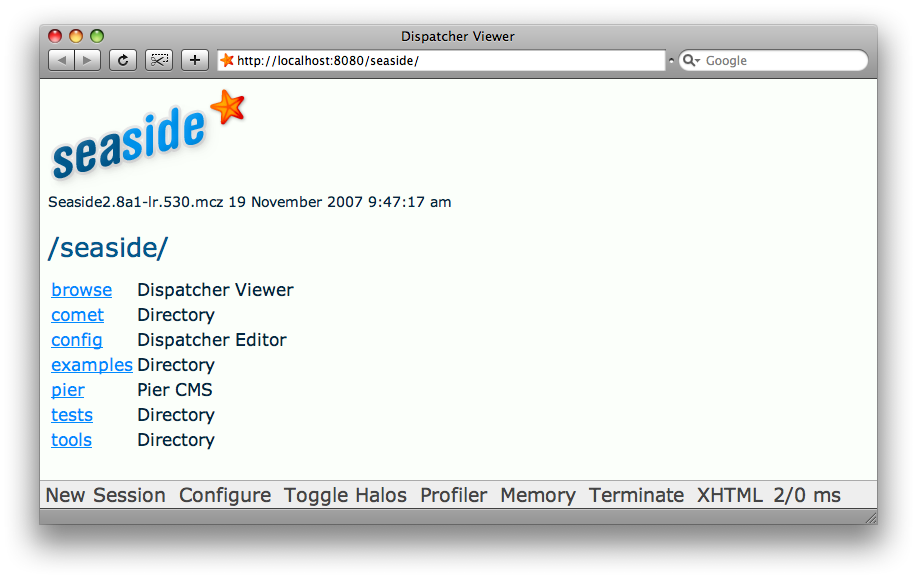
\includegraphics[width=\textwidth]{seasideStartup}
\caption{Seasideの初期画面
}
\figlabel{seasideStartup}
\end{center}
\end{figure}

\dothis{Seasideを開始してWebブラウザのURLを \url{http://localhost:8080/seaside/}にします。}

\noindent
\figref{seasideStartup}のようなページが表示されます。

\noindent
\dothis{\lct{examples{\go}counter}ページをクリックしてください。 (\figref{counter})}


\begin{figure}[htb]
\begin{center}
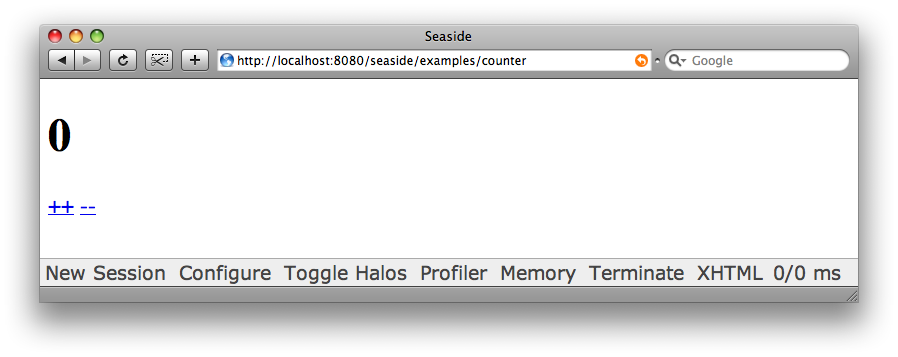
\includegraphics[width=0.8\textwidth]{counter}
\caption{カウンターのアプリケーション}
\figlabel{counter}
\end{center}
\end{figure}

\noindent
これはSeasideアプリケーションのサンプルです。\link{++}や \link{--\,--}のリンクをクリックするとカウンターの値を変えることができます。

\noindent
\dothis{リンクをクリックして値を変えてみましょう。Webブラウザの「戻る」ボタンで前の状態に戻ってから\link{++}のリンクをまたクリックしてみてください。
カウンターは、ちゃんと表示されていた値から増えています。決して「戻る」ボタンを押し始めたときの値からではないのです。}


今度は図\figref{seasideStartup}の\subind{Seaside}{toolbar}の初期画面の下のほうにあるツールバーに注目してみてください。
Seasideは「セッション」の概念をサポートしており、各アプリケーションはユーザごとに状態を管理できるようになっています。
\button{New Session} を押すと、アプリケーションの新たなセッションが始まります。
\button{Configure} ではアプリケーションの各種設定をWebブラウザ経由で行うことができます。

(\button{Configure}の画面を閉じるには、右上の \link{x} リンクをクリックします)。
\button{Toggle Halos} を押すと、Seasideで動作しているアプリケーションの状態を調べていくことができます。
\button{Profiler} と \button{Memory} ボタンはアプリケーション実行時のパフォーマンスに関する詳細な情報を見るためのものです。

\button{XHTML} は生成されたWebページのXHTMLをバリデートするときに使います。該当ページが外部からアクセス可能になっていないとこの機能は動作しません。W3Cのバリデータを使っているからです。
\index{Seaside!halos}

Seasideのアプリケーションは付け外し可能な「コンポーネント」からできています。Seasideのフレームワークが提供する\ct{WAComponent}クラスを継承したクラスのインスタンスであるということを除けば、実のところコンポーネントは通常のSmalltalkのオブジェクトです。\pharo のイメージからコンポーネントやクラスを探索できますし、Webブラウザからハローを通じて直接たどっていくこともできます。

\begin{figure}[ht]
\begin{center}
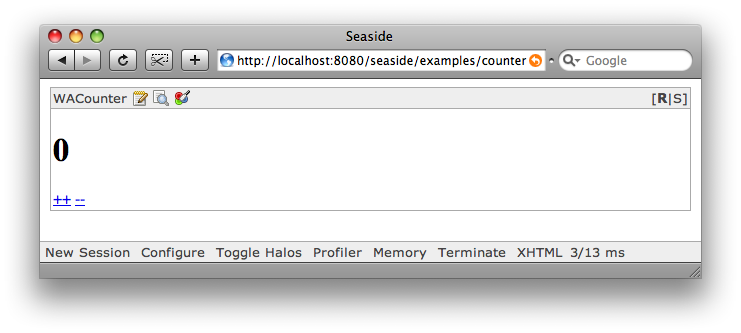
\includegraphics[width=\textwidth]{counterHalos}
\caption{ハロー}
\figlabel{counterHalos}
\end{center}
\end{figure}

\dothis{\button{Toggle Halos}を押してみましょう。\figref{counterHalos}のような画面になるはずです。
左上に\ct{WACounter}と表示されていますが、これは現在のページの構成要素となっているコンポーネントのクラス名を表しています。 
隣には3つのボタンアイコンがあります。
最初の鉛筆のアイコンは、このコンポーネントのクラスブラウザを開くためのものです。2番目の虫眼鏡アイコンでは、現在アクティブになっている\ct{WACounter}のインスタンスのインスペクタを開くことができます。
3番目の色のついた丸のボタンを押すと、コンポーネントについての\ind{CSS} スタイルシートエディタが表示されます。
右上には\link{R} と \link{S}のリンクがあります。それぞれクリックするとコンポーネントが通常表示とソース表示とに切り替わります。
こうしたリンクをすべて試してみましょう。
ソースビューの表示のときにも、\link{++} や \link{{-}{-}}は有効になっています。フォーマットもされているため、Webブラウザでソース表示をしたときよりも見やすいかもしれません。}

Seasideのクラスブラウザやオブジェクト・インスペクタは、サーバが別のマシンで動作していて、画面がなかったり、遠く離れていたりするときには非常に便利です。
とはいえ、最初にSeasideのアプリケーションを開発するときには、ローカルでサーバを動かすと思います。その場合は\pharoのイメージが提供する通常の開発ツールのほうが使いやすいでしょう。

\begin{figure}[ht]
\begin{center}
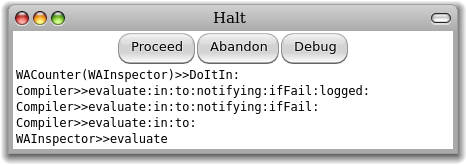
\includegraphics[width=0.7\textwidth]{haltingCounter}
\caption{カウンターアプリをhaltさせる}
\figlabel{haltingCounter}
\end{center}
\end{figure}

%\dothis{Using the object inspector link in the web browser, open an inspector on the underlying Smalltalk counter object and evaluate \ct{self halt}}.
\dothis{Webブラウザのオブジェクト・インスペクタのリンクを使い、カウンターのインスペクタを開けてみて、 \ct{self halt}を実行してみましょう。
Webページはロード途中の状態になります。Seasideのイメージのほうに移ってみてください。ノーティファイアが上がっていて (\figref{haltingCounter})、  \ct{WACounter} のオブジェクトが \ct{halt} の実行で止まっていることが確認できます。
さらにデバッガを開いて \button{Proceed} を押してみましょう。Webブラウザに戻るとカウンターは再び動作しています。}

Seasideのコンポーネントは、異なるコンテキストで何度も初期化できます。

\begin{figure}[ht]
\begin{center}
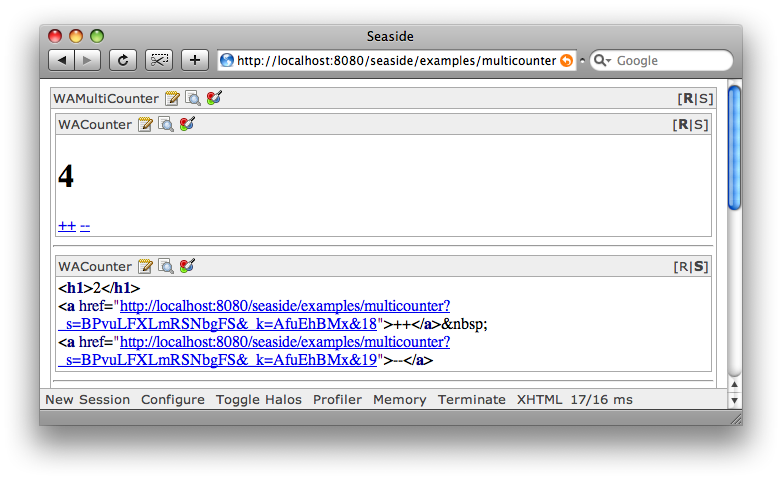
\includegraphics[width=\textwidth]{multiCounterHalos}
\caption{独立したサブコンポーネント}
\figlabel{multiCounterHalos}
\end{center}
\end{figure}

%\dothis{Point your web browser to \url{http://localhost:8080/seaside/examples/multicounter}}.
\dothis{WebブラウザのURLを\url{http://localhost:8080/seaside/examples/multicounter}に指定してみてください。
いくつもの独立したカウンターコンポーネントからなるアプリケーションが立ち上がります。
カウンターをいくつか選んで値を変えてみましょう。「戻る」ボタンを押しても問題なく動作します。
ハローを表示してみると、入れ子になったコンポーネントからアプリケーションができていることがわかります。クラスブラウザを使って、 \ct{WAMultiCounter}の実装がどうなっているか見てみましょう。
クラスメソッドが3つ(\ct{canBeRoot}、 \ct{description}、 \ct{initialize})、インスタンスメソッドも3つ(\ct{children}、 \ct{initialize}、 \ct{renderContentOn:})定義されていることがわかります。
アプリケーションでは、クラスメソッドの\ct{canBeRoot}で \ct{true}を返すことで、コンポーネント階層のルートになり得るという宣言を行っています。}
\index{Seaside!multi-counter}

SeasideのWebインターフェースを使うと、アプリケーション(\ie ルートになっているコンポーネント)を設定したり、コピーしたり、登録解除したりできます。設定を少しいじってみましょう。

\dothis{Webブラウザで\url{http://localhost:8080/seaside/config}を開きます。ユーザIDとパスワードを入れて、ログインしてください。(デフォルトでは\ct{admin} / \ct{seaside} となっています)。
``examples''の隣にある \link{Configure} をクリックします。 ``Add entry point''のところで、 ``counter2''と名前を入れ、タイプは \emph{Application} のまま \button{Add}ボタンをクリックします( \figref{counter2}を参照)。
次の画面で、 \emph{Root Component} を \clsind{WACounter}にして、 \button{Save} を押して、 \button{Close}で閉じます。
これでカウンターの新しいアプリケーションが \url{http://localhost:8080/seaside/examples/counter2}で起動するようになりました。
同様に、この設定ツール画面を通じてアプリケーションの登録解除を行うこともできます。
}
\index{Seaside!configuration}


\begin{figure}[ht]
\begin{center}
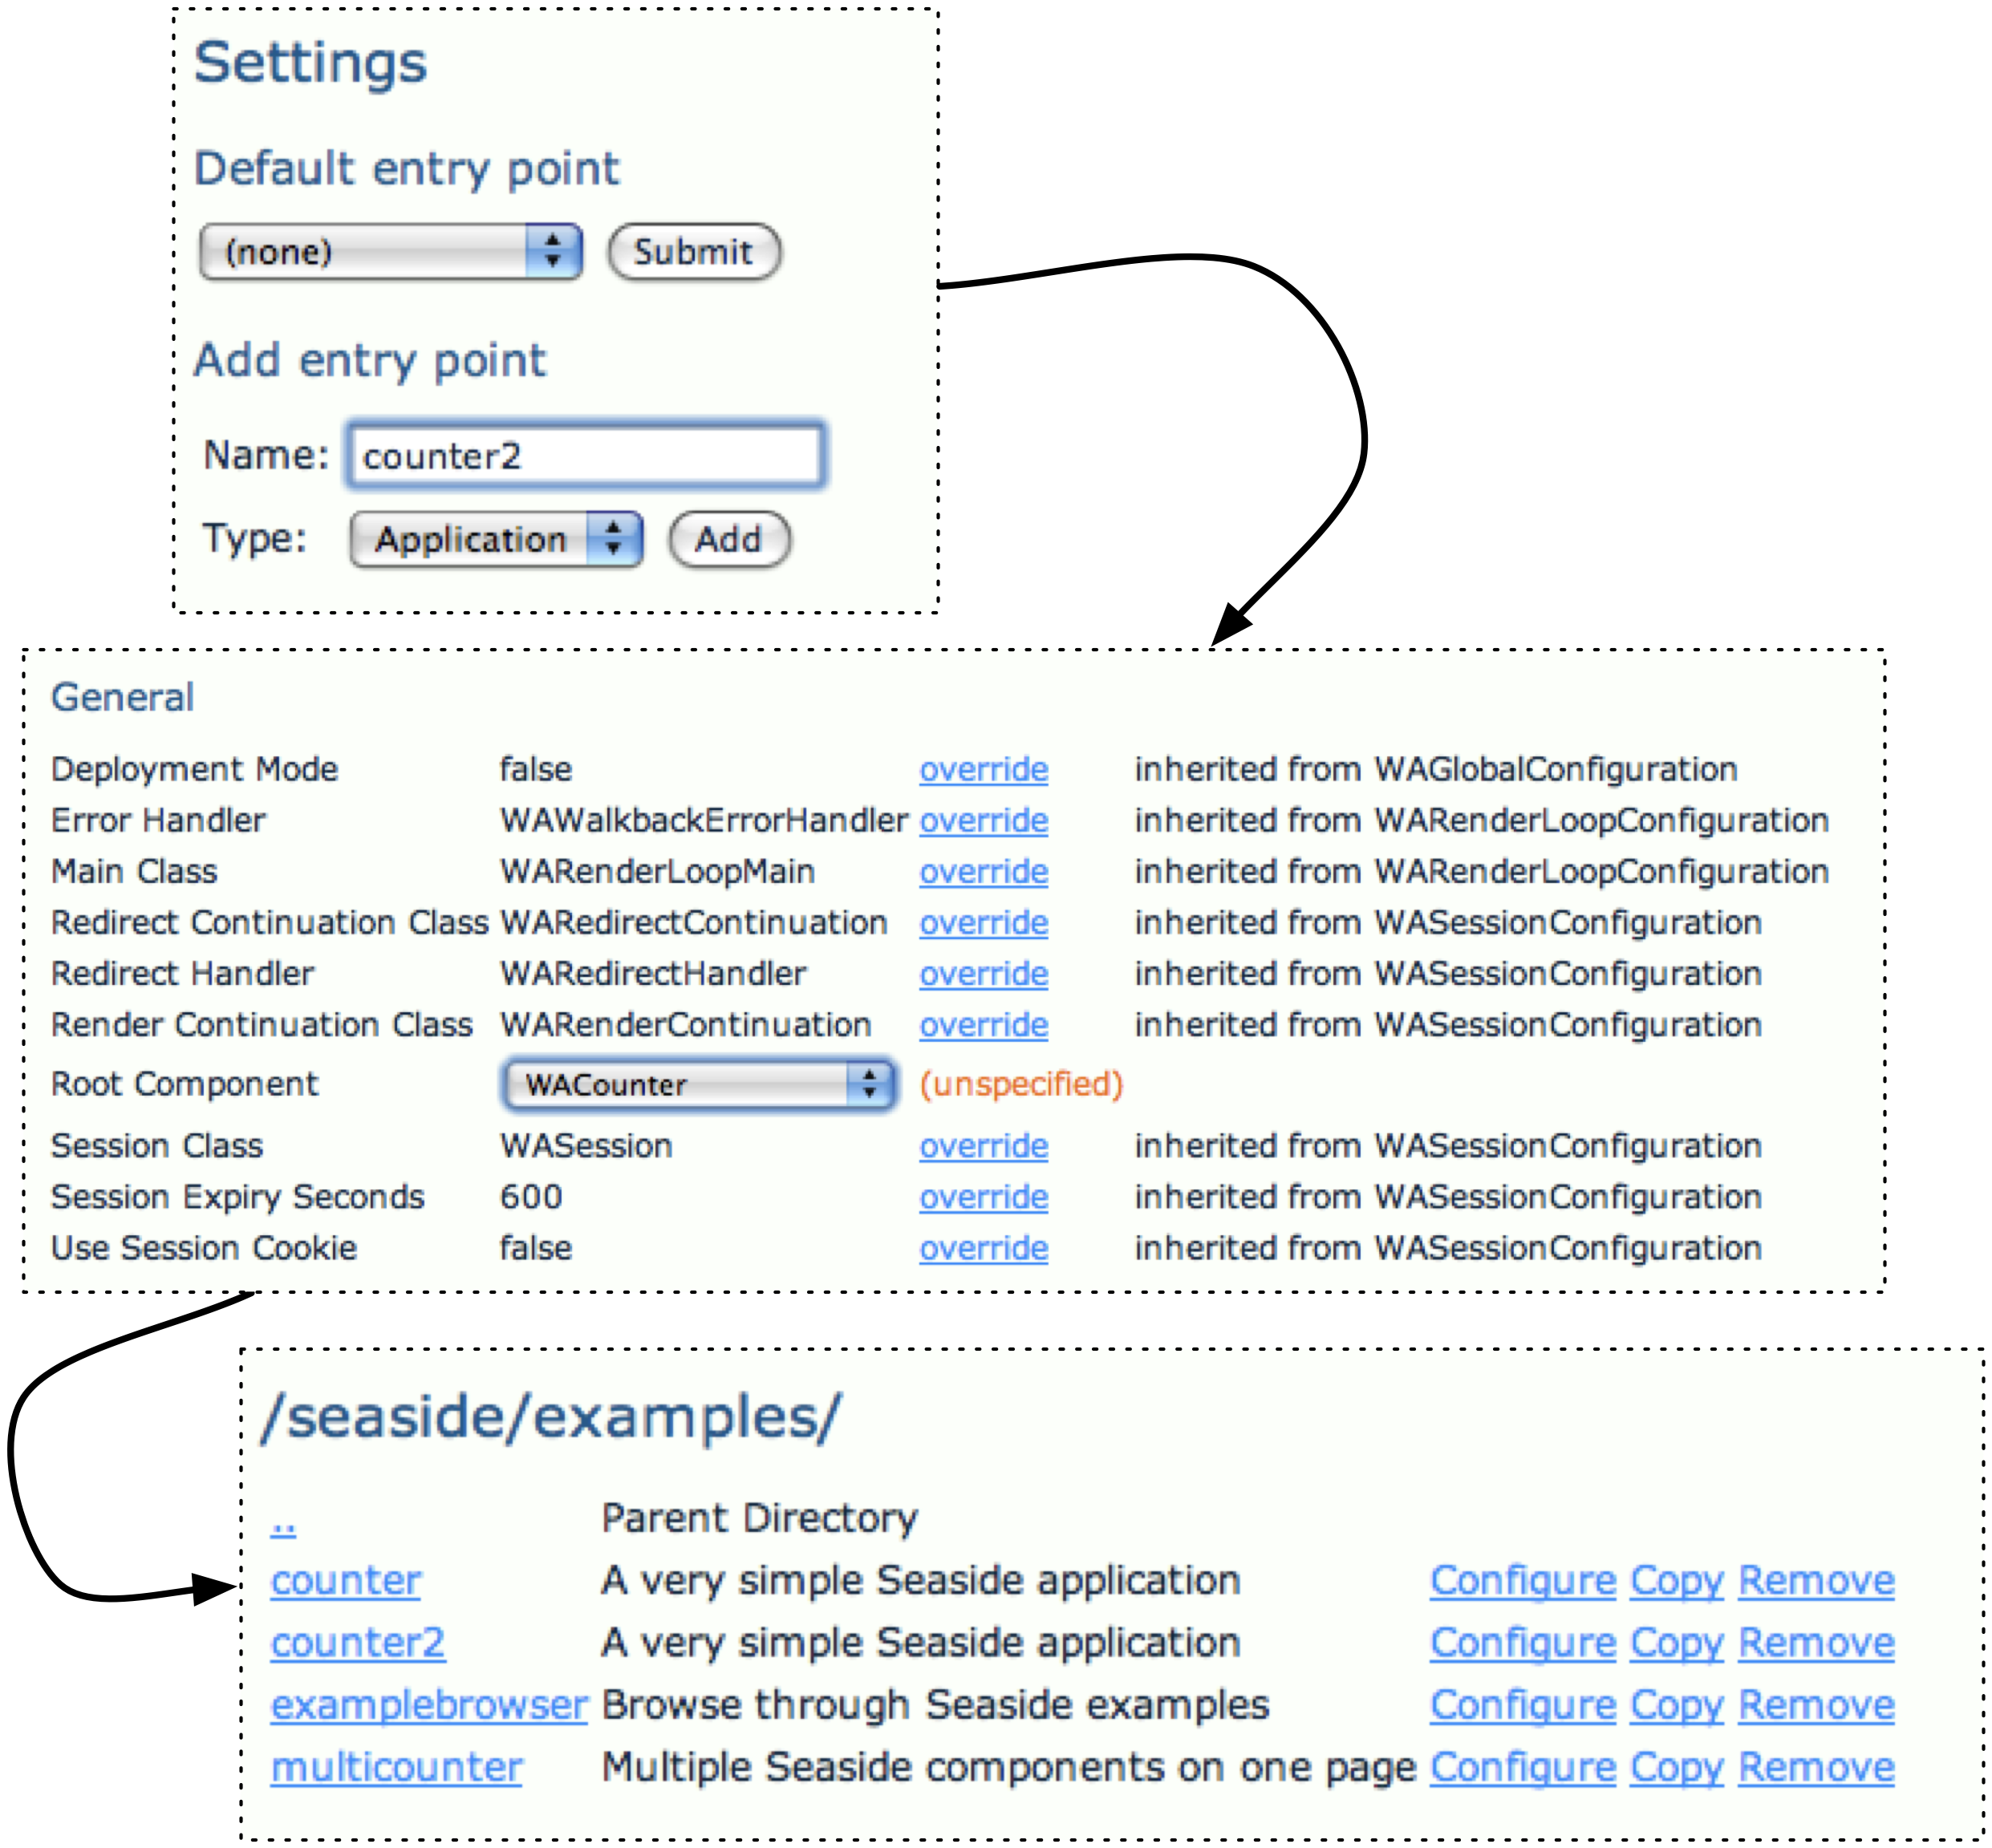
\includegraphics[width=\textwidth]{counter2}
\caption{新たなアプリケーションの設定}
\figlabel{counter2}
\end{center}
\end{figure}

Seasideは2つのモードで動作します。一つは今まで見てきた \emph{開発}モードです。 \emph{デプロイ} モードにすると、画面下のツールバーが非表示となります。
\index{Seaside!deployment mode}
\index{Seaside!development mode}

デプロイモードにするには、全体の設定ツールのページからアプリケーションを選んで、 \link{Configure} をクリックするか、ツールバーに表示されている \link{Configure} をクリックします。
% \ab{How?  I couldn't find this}
どちら場合も、デプロイモードのプルダウンボックスが表示されるので、\emph{true}に設定します。
この設定は新たなセッションを開始したタイミングで有効になります。
Seaside全体でモードを切り替えるには\clsind{WAGlobalConfiguration} \lct{setDeploymentMode}や、\ct{WAGlobalConfiguration setDevelopmentMode}を実行します。
\index{Seaside!deployment mode}
\index{Seaside!development mode}


設定ツール自体もSeasideのアプリケーションです。そのため同じようにWebブラウザから各種の設定ができます。もしも誤って``config'' のアプリケーションを削除してしまった場合は、
\clsind{WADispatcherEditor} \ct{initialize} とすると元に戻ります。

%=================================================================
\section{Seasideのコンポーネント}
\seclabel{components}

%\ab{This section was too long\,---\,18 pages.  It also contained several self-references (``see section 1.3''). So I broke into smaller sections, by promoting some of the subsections and subsubsections.}

前の節で示したように、Seasideのアプリケーションは\emph{\subind{Seaside}{コンポーネント}}から成り立っています。
\emph{Hello World}のコンポーネントを作成し、Seasideの仕組みをさらに詳しく見てみましょう。
コンポーネントを定義するには \clsind{WAComponent}を直接あるいは間接的に継承するようにします(\figref{WACounter})。

\dothis{ \ct{WAComponent}を継承した \ct{WAHelloWorld}クラスを定義してみましょう。}

コンポーネントでは自身の表示の仕方を定める必要があります。
このためには\mthind{WAPresenter}{renderContentOn:}をオーバーライドします。引数として XHTMLの生成方法を知っている\clsind{WAHtmlCanvas}が渡ってくるようになっています。
\index{Seaside!rendering}

\dothis{ \prot{rendering}プロトコルに以下のようにメソッドを定義してみましょう。}
\needlines{2}
\begin{code}{}
WAHelloWorld>>>renderContentOn: html
	html text: 'hello world'
\end{code}

\noindent
次に Seasideに対して、コンポーネントがスタンドアロンのアプリケーションであるという宣言を行います。

\dothis{\ct{WAHelloWorld} のクラス側に以下のメソッドを定義しましょう。}

\begin{code}{}
WAHelloWorld class>>>canBeRoot
	^ true
\end{code}

\noindent
ほとんどこれでできあがりです。

\dothis{Webブラウザで \url{http://localhost:8080/seaside/config}を開き、 ``hello''のエントリポイントを追加し、ルートのコンポーネントを \ct{WAHelloWorld}に設定します。
そしてURLを\url{http://localhost:8080/seaside/hello} に変えると、 \figref{WAHelloWorld}}のように表示されています!

\begin{figure}[htb]
\begin{center}
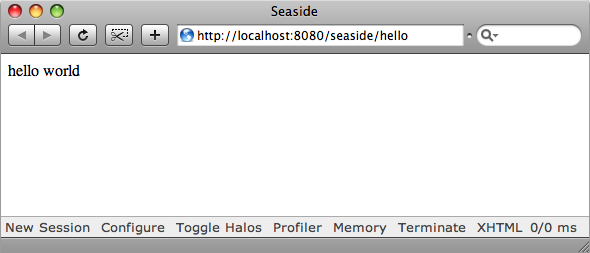
\includegraphics[width=\textwidth]{WAHelloWorld}
\caption{Seasideの``Hello World''}
\figlabel{WAHelloWorld}
\end{center}
\end{figure}

%-----------------------------------------------------------------
\subsection{状態のバックトラックと``Counter''アプリケーション}
%{Simple and nested components}

``hello world''に比べて、「カウンター」のアプリケーションは、ほんの少しだけ難しいものになっています。
\seclabel{backtracking}

\begin{figure}[ht]
\begin{center}
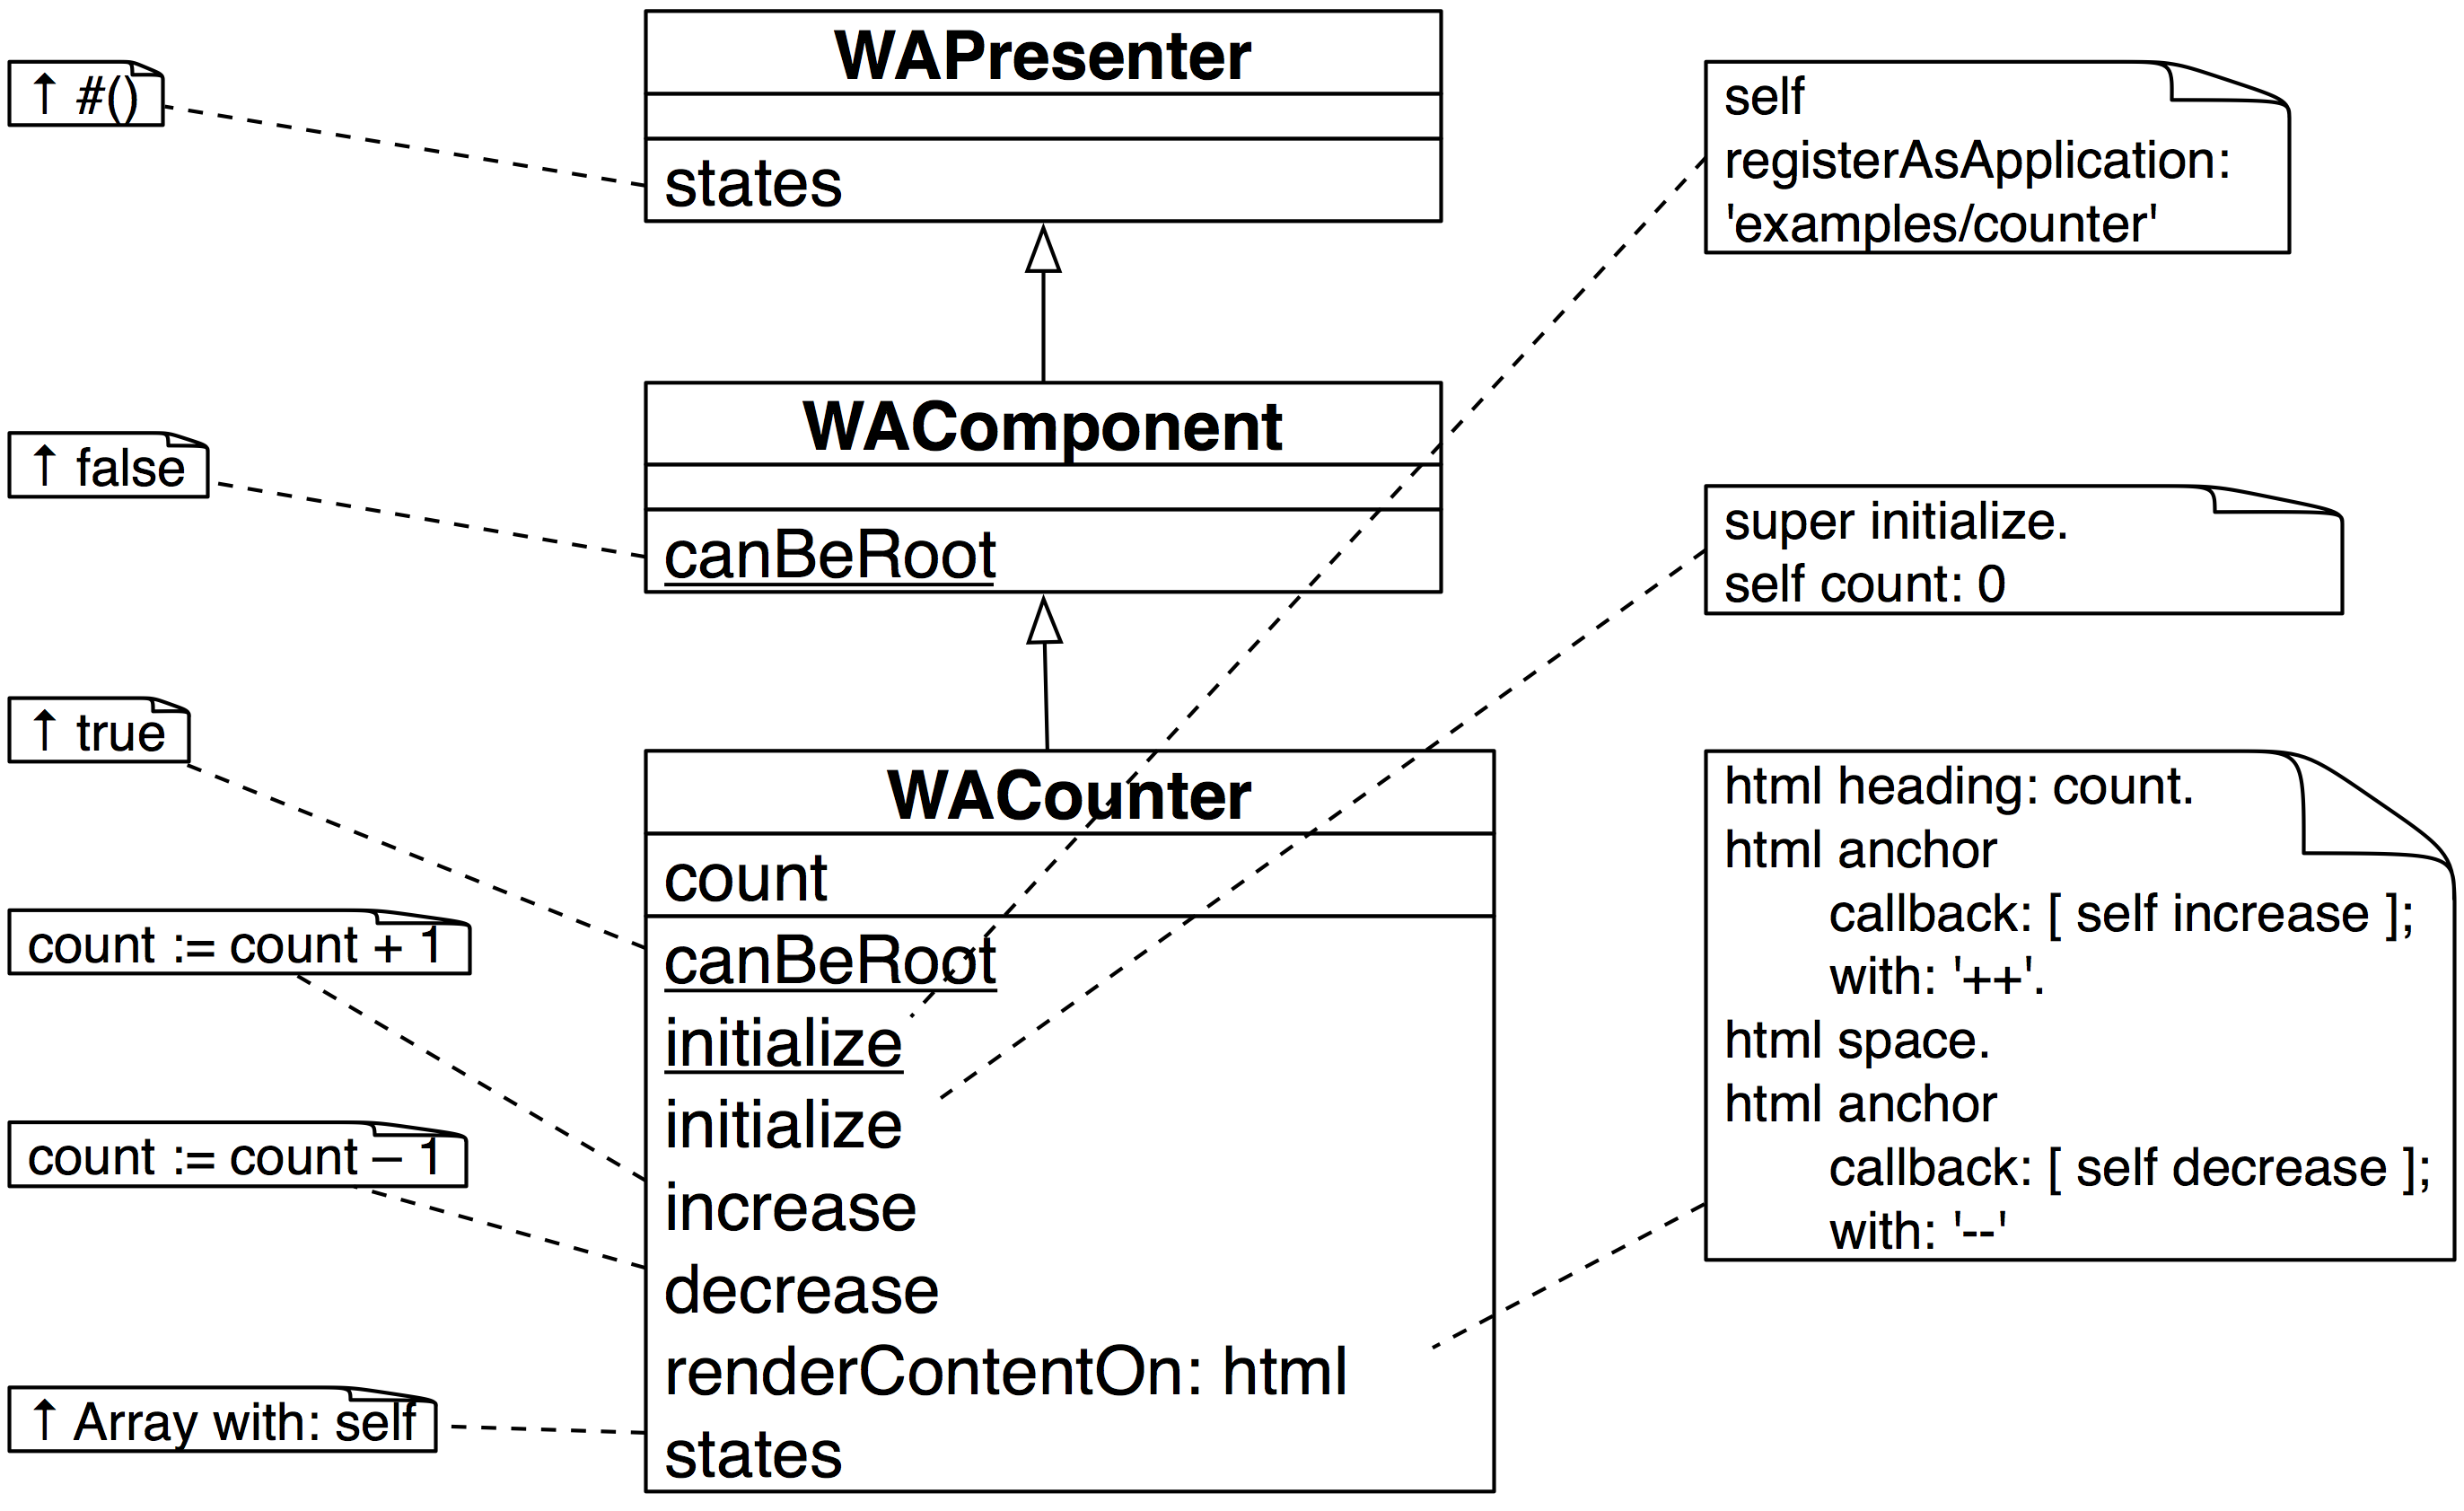
\includegraphics[width=\textwidth]{WACounter}
\caption{\emph{counter}アプリケーションは\ct{WACounter}クラスにより実装されています。  アンダーラインの引いてあるメソッドはクラスメソッドです。}
\figlabel{WACounter}
\end{center}
\end{figure}

 \clsind{WACounter} はスタンドアロンのアプリケーションなので \ct{WACounter class} では  \mthind{WAComponent class}{canBeRoot} を実装して、\ct{true} を返す必要があります。
 アプリケーションとしての登録は、図 \figref{WACounter}にあるように、クラスメソッド \ct{initialize}の中で行われています。 

\ct{WACounter} には \ct{increase} と \ct{decrease}メソッドがあります。それぞれWebページで \link{++} 、 \link{--\,--} のリンクをクリックしたときに呼び出されます。カウンターの値を保持するため、インスタンス変数としては \ct{count}が定義してあります。
「戻る」ボタンを押してもカウンターの値がブラウザの値とずれないようにするには、\ct{WACounter} の状態をバックトラックするようにしなければなりません。
Seasideは、バックトラックのためのメカニズムを最初から持っていますが、アプリケーションのどの部分をバックトラックさせるかは開発者が指定する必要があります。

インスタンスメソッドの\ct{states}を実装すると、どの部分をバックトラック対象とするかを定めることができます。
% \ab{note that xspace messes up again, by inserting a space at the start of this line}
\ct{states} では対象とすべきオブジェクト群を配列の形で返すようにします。カウンターアプリケーションの場合、 \ct{Array with: self}としています。こうすると \ct{WACounter} のオブジェクト自身がSeasideにバックトラック対象として登録されることになります。

\paragraph{\emph{注意}}
バックトラック対象のオブジェクトの宣言ではちょっとした注意点があります。
Seasideは配列内のオブジェクトの\emph{copy}を取ることで、過去の状態を保持します。

実際の処理は \clsind{WASnapshot} によって行われます。 \ct{WASnapshot}は \clsind{IdentityDictionary} のサブクラスで、バックトラック対象のオブジェクト群をキーに、シャローコピーされたオブジェクト群を値として持っています。
特定のスナップショットに状態を戻す必要があるときには、シャローコピーされた情報を使って、オブジェクトの変数の値を上書きします。
先ほどの\ct{WACounter}の場合、バックトラックの対象は、インスタンス変数\ct{count} の数字だけで良いのではと思うかもしれません。しかし、  \ct{states} メソッドでr\ct{Array with: count} のように書いてもうまく動作しないのです。
これは\ct{count}の中身が整数で、整数は不変のオブジェクトだからです。
 \ct{increase} や \ct{decrease} メソッドでは、オブジェクトのそのものが \ct{0}から \ct{1} になったり、 \ct{3}から \ct{2}になっているわけではありません。
 \ct{count} 変数の中身が代入されて別の整数になっているのです。整数が増えたり減ったりするたびに、 \ct{count} が指すオブジェクトは 別のものに\emph{成り代わって}います。このため、 \ct{WACounter>>>states}では\ct{Array with: self}と書く必要があるのです。 \mbox{\ct{WACounter}} が以前の状態に戻るときには、各インスタンス変数の値がコピーされた\mbox{\ct{WACounter}}から復元されます。これで \ct{count} の値は正しく戻ることになります。
\index{Seaside!backtracking state}
\index{WAPresenter!states@\ct{states}}

\section{XHTMLのレンダリング}

Webアプリケーションでは、Webページを動的に生成して表示(レンダリング)を行います。 \secref{コンポーネント}の節で述べたように、Seasideのコンポーネントは、それぞれが自身をレンダリングするようになっています。
レンダリングの仕組みを知るため、カウンターのコンポーネントがどのようにレンダリングを行っているか、見ていきましょう。

\subsection{カウンターのレンダリング}

カウンターのレンダリングは比較的単純です。 \figref{WACounter}のコードを見てください。
カウンターの現在の値がXHMLTの見出しとして表示されます。値の増減の操作はアンカー(リンク)として実装されていて、コールバックがブロックの形で仕掛けられています。アンカーをクリックすると \ct{increase} や \ct{decrease}がカウンターオブジェクトに対して送られるようになっています。

レンダリングで送るメッセージ群についてはすぐ後で詳しく解説しますが、その前に\subind{Seaside}{マルチカウンター}のほうもどうなっているか見てみましょう。

\subsection{CounterからMultiCounterへ}

まず \figref{WAMultiCounter} で示すように\ct{WAMultiCounter}もスタンドアロンのアプリケーションなので、 \mthind{WAComponent class}{canBeRoot}を実装して \ct{true}を返すようにしています。

マルチカウンターのコンポーネントは、サブコンポーネントを含んだ \emph{コンポジット} となっています。そのため \ct{children} メソッドを実装して、中に含まれるコンポーネント群を配列の形で返すようにしています。

レンダリングでは、サブコンポーネントの表示を、水平線で区切りながら行うように書いています。
そのほか初期化を行うためのインスタンスメソッド、クラスメソッドがありますが、基本的にはこれだけで良いのです!

\begin{figure}[bht]
\begin{center}
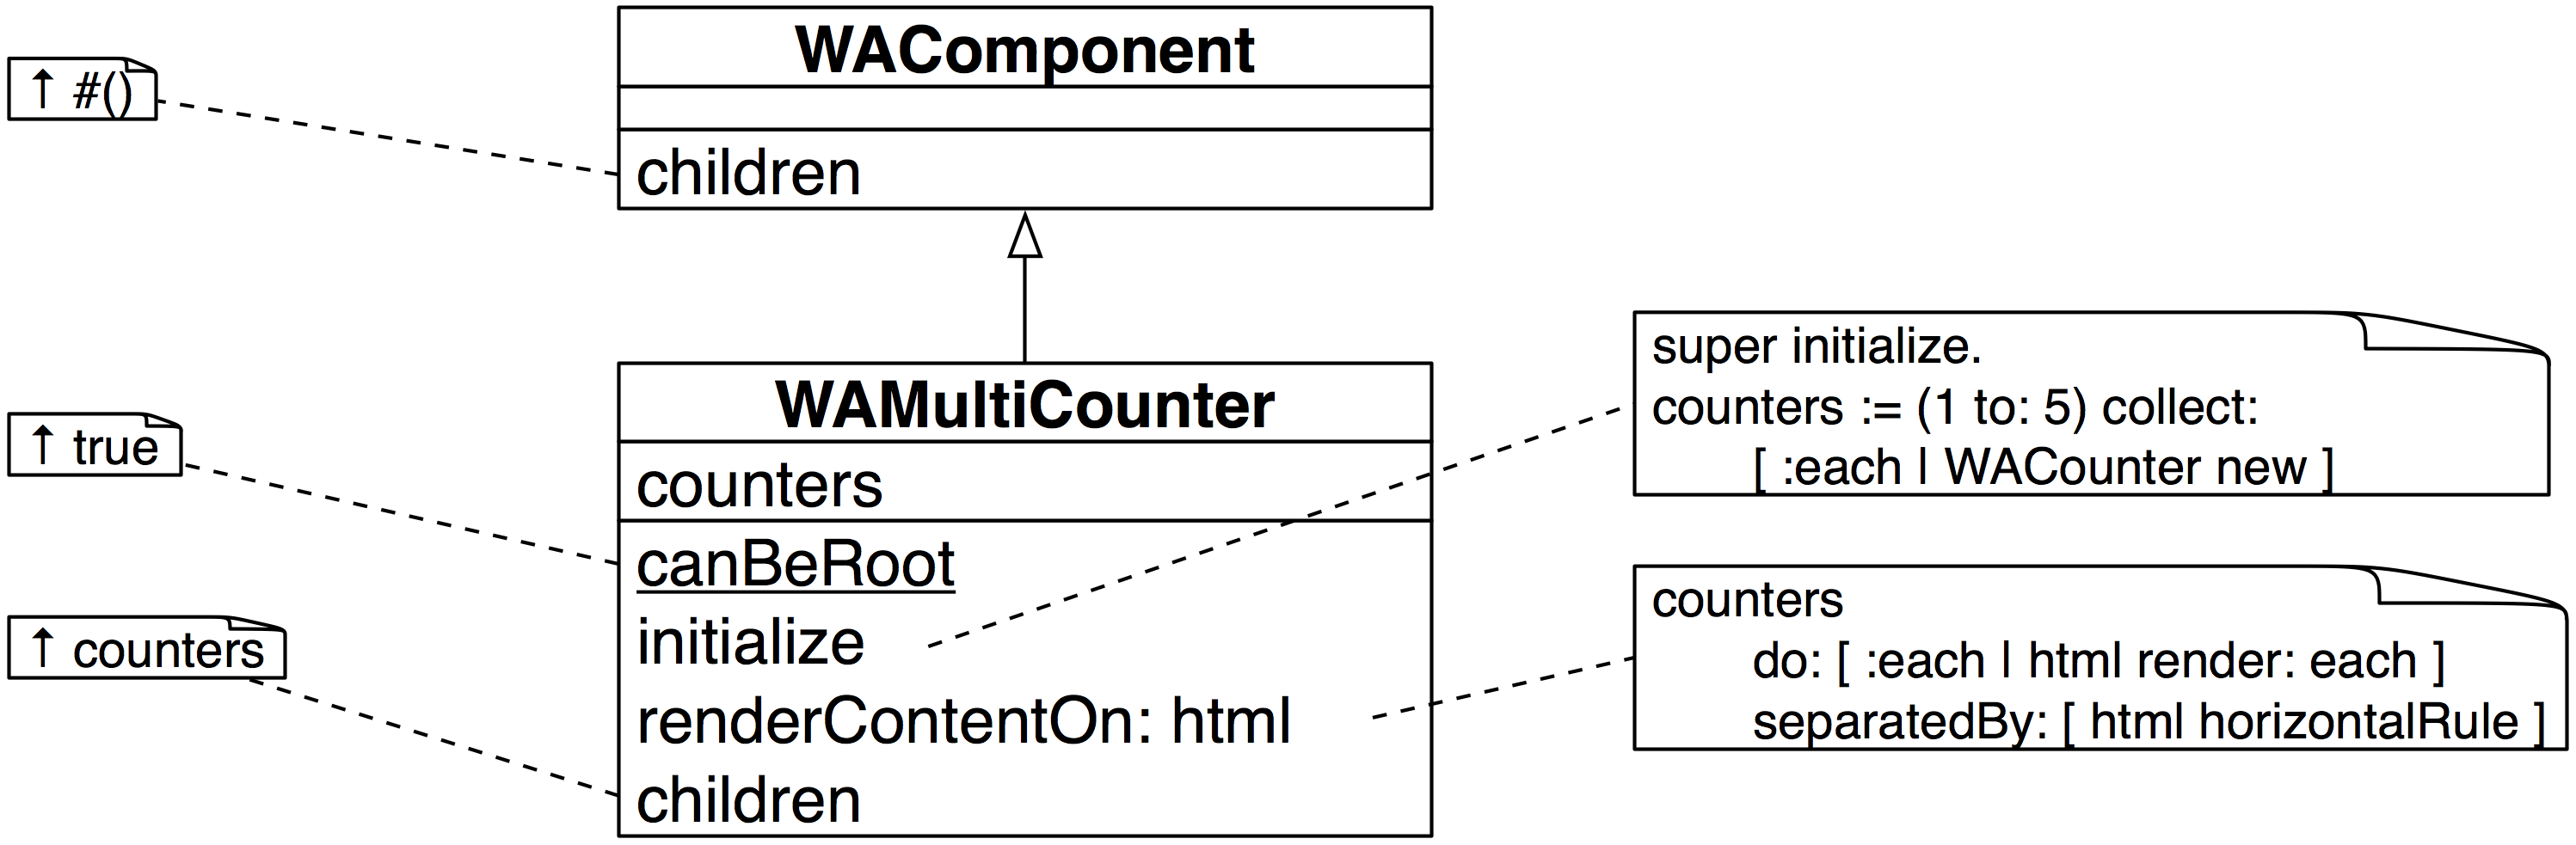
\includegraphics[width=\textwidth]{WAMultiCounter}
\caption{WAMultiCounter}
\figlabel{WAMultiCounter}
\end{center}
\end{figure}

%-----------------------------------------------------------------
\subsection{レンダリング詳細}

今までの例で見てきたように、SeasideではWebページ生成でテンプレートを使いません。Smalltalkのメッセージ送信で生成するのです。
Seasideのコンポーネントは  \mthind{WAPresenter}{renderContentOn:}をオーバーライドする決まりになっています。このメソッドはフレームワークの側からコンポーネントのレンダリングのときに呼び出されます。
\ct{renderContentOn:} は、引数を一つ取りますが、 \seeindex{canvas}{htmlキャンバス} \emphind{htmlキャンバス}オブジェクトが渡ってくるようになっています。これを使ってコンポーネントはレンダリングを行います。慣習によりキャンバスは \ct{html} という名前になっています。htmlキャンバスはMorphicや別のGUIフレームワークでのキャンバスに似ています。デバイス固有となる描画の詳細を隠す役割を持っています。

基本的なレンダリングメッセージをいくつか挙げてみます。
\begin{code}{}
html text: 'hello world'.  "テキストを表示"
html html: '&ndash;'.     "XHTMLの直接指定"
html render: 1.              "オブジェクトのレンダリング"
\end{code}

\ct{任意のオブジェクト}を表示するのに \ct{render: anObject} を使うことができます。通常はサブコンポーネントの表示で使われます。引数となった \lct{anObject}には \ct{renderContentOn:}のメッセージが内部的に送られます。
マルチカウンターの例で使いました ( \figref{WAMultiCounter}を参照)。

\subsection{ブラシの利用}
\seclabel{brushes}

キャンバスでは描画を行うため、たくさんの \emphind{ブラシ} を使うことができます。
XHTMLの各要素(段落、テーブル、リストなど)に対応したブラシがあります。
ブラシやそれに関連する便利メソッドを知るには、\clsind{WACanvas} とそのサブクラスをブラウズすると良いでしょう。
 \ct{renderContentOn:} の引数は、\clsind{WACanvas}を継承した \clsind{WARenderCanvas}のインスタンスになっています。

すでにカウンターとマルチカウンターの例で、以下のブラシを使いました。
\needlines{2}
\begin{code}{}
html horizontalRule.
\end{code}

\begin{figure}[ht]
\begin{center}
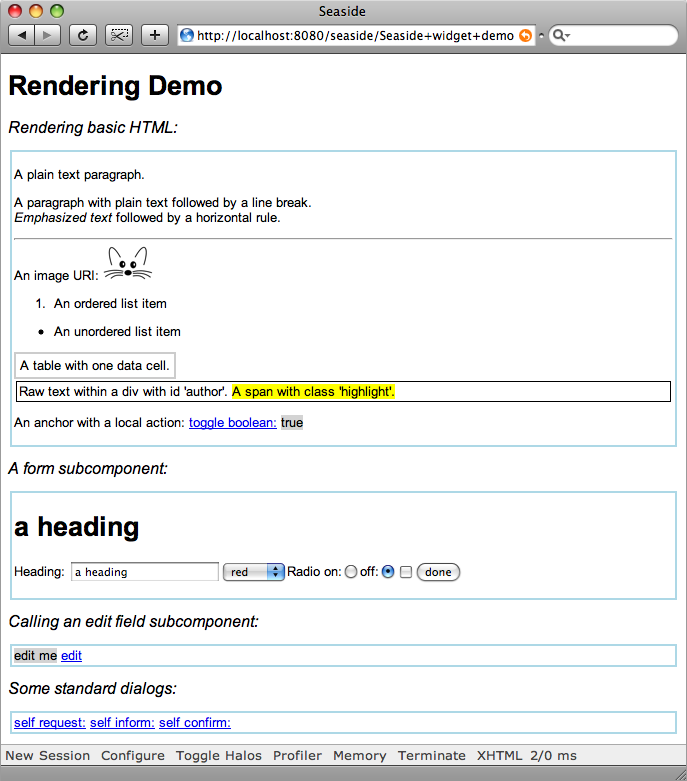
\includegraphics[width=\textwidth]{RenderingDemo}
\caption{レンダリングのデモ}
\figlabel{RenderingDemo}
\end{center}
\end{figure}

図 \figref{RenderingDemo}は、Seasideが提供する基本的なブラシをいろいろ使ってみた例です。 \footnote{
 \mthref{renderdemo}のソースコードは  \url{http://www.squeaksource.com/PharoByExample}プロジェクトの\ct{PBE-SeasideDemo}パッケージ内にあります。} \ct{SeasideDemo} のルートコンポーネントは単にサブコンポーネントの表示を行うだけです。サブコンポーネントは \mthref{renderdemo}を読むとわかりますが、\ct{SeasideHtmlDemo}、 \ct{SeasideFormDemo}、\ct{SeasideEditCallDemo} 、\ct{SeasideDialogDemo}となっています。
 
\needspace{7ex}
\begin{method}[renderdemo]{\lct{SeasideDemo>>renderContentOn:}}
SeasideDemo>>>renderContentOn: html
	html heading: 'Rendering Demo'.
	html heading
		level: 2;
		with: 'Rendering basic HTML: '.
	html div
		class: 'subcomponent';
		with: htmlDemo.
	"render the remaining components ..."
\end{method}

\noindent
コンポーネントはサブコンポーネントを返すようにするというのを覚えているでしょうか。Seasideはレンダリングのたびにサブコンポーネントを再利用します。
\begin{code}{}
SeasideDemo>>>children
	^ { htmlDemo . formDemo . editDemo . dialogDemo }
\end{code}

上記のコードでは \ct{heading} ブラシの使い方が少し違っていることに注意してください。\ct{heading:}は、生成とともに、テキストを直接メッセージの引数でセットする書き方になっています。次に出てくるのは、\ct{heading}メッセージを送りブラシを生成してから、さまざまなプロパティをカスケードでセットしていくというものです。ブラシはたいていこの2種類の書き方ができるようになっています。

\important{もしも \ind{カスケード}を使って、ブラシに \mthind{WABrush}{with:}を送るのであれば、 \ct{with:} は必ず\emph{最後に}書く必要があります  message.
\ct{with:} によってブラシのレンダリングが始まるからです。}

\mthref{renderdemo}のメソッドでは、最初の見出しはデフォルトのレベル1になります。次の見出しではレベルを2に明示的に設定しています。
 サブコンポーネントはXHTMLで\emph{div}の中に囲まれる形になります。divには ``subcomponent''という\ind{CSS}のクラスを付与しています(CSSの使い方については\secref{css}で解説します)。  \ct{with:} メッセージの引数は、文字列とは限りません。この例ではコンポーネントを渡しています。次の例でも出てきますが、レンダリングの操作を記述したブロックでも良いのです。

\ct{SeasideHtmlDemo}コンポーネントは 基本的なブラシをいろいろと使ったデモになっています。コードを見ればだいたい利用法がわかるでしょう。

\begin{code}{}
SeasideHtmlDemo>>>renderContentOn: html 
	self renderParagraphsOn: html.
	self renderListsAndTablesOn: html.
	self renderDivsAndSpansOn: html.
	self renderLinkWithCallbackOn: html
\end{code}

上のように、レンダリングのメソッドが長くなった場合には細かいメソッド群に分割することがよく行われます。

\important{一つのメソッド内に長々とレンダリング処理を書くやり方はお勧めできません。\ct{render*On:}という形でヘルパーメソッドとして分割しましょう。そうしたメソッド群は\prot{rendering} メソッドカテゴリーに置いておくようにします。また、 コンポーネントに\ct{renderContentOn:}を直接送ってはいけません。代わりに\ct{render:}を送りるようにしてください。}

さらにコードを見ていきましょう。

最初の\ct{SeasideHtmlDemo>>>renderParagraphsOn:}ヘルパーメソッドは、XHTMLの段落、通常のテキスト、強調表示されたテキスト、画像の表示の仕方の例になっています。

Seasideでは単純な要素であれば単に文字列を指定するだけでレンダリングできますし、複雑なものであればブロックを使います。レンダリングのコードを書くときの指針として覚えておくと良いでしょう。

\begin{code}{}
SeasideHtmlDemo>>>renderParagraphsOn: html 
	html paragraph: 'A plain text paragraph.'.
	html paragraph: [
		html
			text: 'A paragraph with plain text followed by a line break. ';
			break;
			emphasis: 'Emphasized text ';
			text: 'followed by a horizontal rule.';
			horizontalRule;
			text: 'An image URI: '.
		html image
			url: self squeakImageUrl;
			width: '50']
\end{code}

次のヘルパーメソッド\ct{SeasideHtmlDemo>>>renderListsAndTablesOn:}は、リストとテーブルの表示例になっています。 テーブルではネストしたブロックを使って、列と列の中のセルを表示させるようにします。

\begin{code}{}
SeasideHtmlDemo>>>renderListsAndTablesOn: html 
	html orderedList: [
		html listItem: 'An ordered list item'].
	html unorderedList: [
		html listItem: 'An unordered list item'].
	html table: [
		html tableRow: [
			html tableData: 'A table with one data cell.']]
\end{code}

次の例は、\emph{div}や \emph{span}の要素に、CSSの \emph{class} や \emph{id} 属性を指定するやり方を示しています。もちろん
 \ct{class:} や \ct{id:} といったメッセージは、\emph{div} \emph{span}以外のブラシにも送ることができます。
\ct{SeasideDemoWidget>>>style} のメソッドで、XHTMLの要素が実際にどのようなスタイルで表示されるかを定義しています(\secref{css}を参照)。

\begin{code}{}
SeasideHtmlDemo>>>renderDivsAndSpansOn: html 
	html div
		id: 'author';
		with: [
			html text: 'Raw text within a div with id ''author''. '.
			html span
				class: 'highlight';
				with: 'A span with class ''highlight''.']
\end{code}

最後に、リンクの簡単な例を見てみましょう。アンカー(リンク) にコールバックを設定しています。リンクをクリックするたびに、文字列が``true''と``false''に切り替わるのですが、これはインスタンス変数の\ct{toggleValue}の値がコールバックの実行で変化するからです。

\needlines{3}
\begin{code}{}
SeasideHtmlDemo>>>renderLinkWithCallbackOn: html 
	html paragraph: [
		html text: 'An anchor with a local action: '.
		html span with: [
			html anchor
				callback: [toggleValue := toggleValue not];
				with: 'toggle boolean:'].
		html space.
		html span
			class: 'boolean';
			with: toggleValue ]
\end{code}

\important{アプリケーションの状態を変えるような処理は、コールバックの中でのみ書くようにします。
レンダリングのコードの中に、直接そのようなコードを書くべきではありません。}

%-----------------------------------------------------------------
\subsection{フォーム}

フォームも今までの例と同様のやり方で表示できます。
図\figref{RenderingDemo}の\ct{SeasideFormDemo} コンポーネントのコードを示します。
\index{Seaside!XHTML forms}

\begin{code}{}
SeasideFormDemo>>>renderContentOn: html
	| radioGroup |
	html heading: heading.
	html form: [
		html span: 'Heading: '.
		html textInput on: #heading of: self.
		html select
			list: self colors;
			on: #color of: self.
		radioGroup := html radioGroup.
		html text: 'Radio on:'.
		radioGroup radioButton
			selected: radioOn;
			callback: [radioOn := true].
		html text: 'off:'.
		radioGroup radioButton
			selected: radioOn not;
			callback: [radioOn := false].
		html checkbox on: #checked of: self.
		html submitButton
			text: 'done' ]
\end{code}{}

フォーム要素は複雑なので、ブロックを使ってレンダリングしています。状態の変更に関わるコードはすべてコールバック内で書かれており、レンダリング部分には書かれないことに注意してください。

 \mthind{WAAnchorTag}{on:of:}については説明が必要でしょう。
上の例ではテキストフィールドに、自身のインスタンス変数\ct{heading}を対応させるために使われています。
アンカーやボタンもこのメッセージに答えられます。

最初の引数はインスタンス変数の名前です。2番目の引数は変数を保持するオブジェクトを指定します。
通常の名前付けルールで、インスタンス変数のアクセッサー (\ct{heading}) とミューテイター (\ct{heading:})がクラスに定義されていることが前提となっています。

このテキストフィールドの例では、デフォルト値を設定したり、新たな値の設定に関するコールバックを設定したりするコードを省くのに役立っています。 \ct{on: #heading of: self}を使うことで \ct{heading} 変数の値はユーザの入力に応じて自動的に更新されます。

すぐ後にコンボボックスの選択で\ct{color} 変数を指定した別の例があります。その後にはチェックボックスの例があり、 \ct{checked} 変数の値が更新されるようになっています。

Seasideの機能テストのコードを見ると、さらにさまざまなフォーム例が見つかります。
%2.8ベース。修正の必要あり(ume) 
% URL -> http://localhost:8080/tests/functional/WAInputPostFunctionalTest
% menu -> WAInputGetFunctionalTest, (WAInputPostFunctionalTest)
 \scat{Seaside-Tests-Functional}のクラスカテゴリを見てみましょう。また、Webブラウザで\url{http://localhost:8080/seaside/tests/alltests}のURLを指定し、
\menu{WAInputTest} を選んで \button{Restart} ボタンを押すと、フォームのほとんどの機能を知ることができます。

ぜひ\button{Toggle Halos}ボタンを押すと、Webブラウザから対応するソースコードにすぐアクセスできるようになるというSeasideの機能を活用してください。

%-----------------------------------------------------------------
\section{CSS: カスケーディング・スタイル・シート}
\seclabel{css}

%\ab{I think that it just needs a few paragraphs telling the reader the key ideas behind CSS, and the new terminology that the CSS folks introduce, before going in to the details of how you define their "thingies".  Now I have forgotten what they call their "thingies" --- I know that there are effectively paragraph styles (divs) and character styles (spans), but I've forgotten what they call them.  So, I think that the text needs to tell the reader, for each thingie, (1) the CSS concept behind the thingie, (2) what it looks like in a CSS style sheet , (3) what it looks like in html, and (4) how to do it in Seaside.   Maybe (3) can be omitted, because it's not needed to use Seaside.}
% \on{I think we do most of that already.}

\ind{CSS}(カスケーディング・スタイル・シート) \footnote{\url{http://www.w3.org/Style/CSS/}}は、Webアプリケーションで、内容と見栄えを分離する方法として標準的なものになってきました。SeasideはCSSの技術を使い、レンダリングのコードが見栄えを意識して煩雑になるのを防いでいます。

コンポーネントは \ct{style}というメソッドを定義することで、使用するスタイルシートを決めることができます。メソッドの中身は単なるCSSの文字列で、コンポーネントが使うスタイルを定めたものにします。

Webページ内に配置されるコンポーネントのスタイルシートは結合されて一つになりますが、各コンポーネントは自身のスタイルを定義で
きます。抽象クラスを定義して、アプリケーションで使う共通のスタイルをメソッドとして定義しておくのも良いでしょう。

しかしデプロイ時には、外部ファイルとしてスタイルシートを用意するのが一般的です。こうするとコンポーネントの機能的な部分と、見栄えの分離がさらに進み、完全に分離されることになります。
( \clsind{WAFileLibrary}クラスを使うと、別途サーバを用意せずに、外部のファイルを利用可能です。)

CSSをよく知っているのでしたら、これで説明は終わりです。念のため、簡単なCSSの紹介を書いておきます。

CSSを使うと、段落やテキストの表示属性を直接Webページに埋め込む代わりに、表示情報を分類分けして、スタイルシートに別途定義できます。段落に該当する要素が \emph{div}で、インラインのテキスト要素は \emph{span} と呼ばれます。
例えば自分で``highlight''といった形で、要素に名前をつけて、ハイライトされるテキストとして定義することもできます(例を参照のこと)。スタイルシートの中では、ハイライトがどのように表示されるべきかを記述します。

基本的に CSS は、XHTMLの要素をどのようなフォーマットで表示するかについて一覧のルールを記述したものです。ルールは二つの部分から成り立っています。
 \emph{セレクター}と呼ばれる部分ではその XHTML 要素にルールを適用するかを指定します。 \emph{宣言} の箇所では、要素に適用される属性の値を定義します。

\begin{figure}[tb]
\begin{code}{}
SeasideDemoWidget>>>style
	^ '
body {
	font: 10pt Arial, Helvetica, sans-serif, Times New Roman;
}
h2 {
	font-size: 12pt;
	font-weight: normal;
	font-style: italic;
}
table { border-collapse: collapse; }
td {
	border: 2px solid #CCCCCC;
	padding: 4px;
}
#author {
	border: 1px solid black;
	padding: 2px;
	margin: 2px;
}
.subcomponent {
	border: 2px solid lightblue;
	padding: 2px;
	margin: 2px;
}
.highlight { background-color: yellow; }
.boolean { background-color: lightgrey; }
.field { background-color: lightgrey; }
'
\end{code}
\caption{\lct{SeasideDemoWidget} 共通スタイルシート
\figlabel{democss}}
\end{figure}

\figref{democss} は、\figref{RenderingDemo}で使われているスタイルシートのメソッドを示したものです。
最初のルールは \ct{body}要素で使われるフォントを指定しています。さらに、見出しレベル2 (\ct{h2})、テーブル (\ct{table})、セル (\ct{td})についての定義が続きます。


残りのルールは、特定の``class'' や ``id''を持つ XHTML要素についてです。クラス属性のCSSのセレクターは``\ct{.}''でid 属性のセレクターは``\ct{#}''で始まります。
classと id の違いは、ページ内でid属性の要素は一つしか存在できませんが(\emph{IDのため})、クラス属性の要素は複数あっても良いということです。 \ct{highlight}はクラス属性なので、ページ内に何度も出てきてかまいません。id属性はページ内で \emph{唯一}の要素、例えばメニュー、更新日、作者の名前などで使われます。また、XHTMLの各要素には、複数のクラス属性が指定できます。その場合は指定された順番に沿って、表示の属性が適用されていきます。

% This style sheet expects at most one element to specify the \emph{author} of the web page.

セレクターは組み合わせることができます。 \ct{div.subcomponent} というセレクターは、divで、クラス属性が``subcomponent''の要素のみを選択することになります。

あまり必要になることはありませんが、ネストした要素を指定することも可能です。例えば ``\ct{p span}''は、段落内(p)のspanを選択します。div内のspanにマッチすることはありません。

CSSについては多くの本やWebページがあります。CSSでどれだけのことができるかを知るには、CSS Zen Garden\footnote{\url{http://www.csszengarden.com/}}のサイトを見てみると良いでしょう。CSSのスタイルシートを変えるだけで、同じ内容の文書をまったく異なったものに見さられるということがわかります。

%-----------------------------------------------------------------
\section{制御フローの管理}

Seaside では、複雑なフローを持つWebアプリケーションを開発するのが、特に簡単にできるようになっています。基本的に二つの仕組みが提供されています。

\begin{enumerate}
  \item コンポーネントは別のコンポーネントを \ct{caller call: callee}のように書いて、\emph{呼び出す}ことができます。呼び出し側は一時的に表示されなくなり、呼ばれた側に制御が移ります。\ct{answer:}によって、制御を元に返すことができます。呼び出し側は定型的には \ct{self}ですが、現在表示されているコンポーネントであればどれでもかまいません。

  \item 全体のワークフローは \emphsubind{Seaside}{タスク}の仕組みで定義できます。\clsind{WAComponent}でなく、\clsind{WATask}を継承することで、特別なコンポーネントになります。 \seclabel{task} タスクは内部にコンポーネントを持ちません。
   \ct{renderContentOn:}を実装する代わりに、 \ct{go} メソッドを定義し、全体の流れを、コンポーネントを順番に \ct{call:}形で書いていきます。
  
\end{enumerate}
\index{Seaside!control flow}

%-----------------------------------------------------------------
\subsection{call:とanswer:}

call:とanuswer:は単純なダイアログ形式のUIを実現するために使われます。

 \ct{call:} と \ct{answer:} を使った簡単な例は、図\figref{RenderingDemo}のレンダリングのデモに含まれています。
 \ct{SeasideEditCallDemo} のコンポーネントはテキストフィールドと \emph{edit}リンクを表示しています。editのリンクにはコールバックが仕掛けられていて、\ct{SeasideEditAnswerDemo}のインスタンスを、テキストフィールドの値で初期化した上で、呼び出すようになっています。コールバックではさらに、呼び出したコンポーネントから受け取った値をテキストフィールドに反映させるようになっています。
 
(以下のコード例では目立たせるために \ct{call:} と \ct{answer:} のメッセージにアンダーラインを引いています。)

\begin{code}{}
SeasideEditCallDemo>>>renderContentOn: html 
	html span
		class: 'field';
		with: self text.
	html space.
	html anchor
		callback: [self text: (self !\underline{call:}! (SeasideEditAnswerDemo new text: self text))];
		with: 'edit'
\end{code}{}

次に表示されるべきWebページ全体を意識する部分がまったくない、というところがエレガントです。実行すると \ct{SeasideEditCallDemo} コンポーネントの部分が \ct{SeasideEditAnswerDemo} コンポーネントに成り代わり、ページ全体の表示が行われます。外側のコンポーネントや隣接するコンポーネントはそのままです。

\important{\mthind{WAComponent}{call:} や \mthind{WAComponent}{answer:} はレンダリングの中に直接記述してはいけません。\subind{Seaside}{コールバック}や、タスクの\mthind{WATask}{go}メソッドの中で書くようにします。}

\ct{SeasideEditAnswerDemo} コンポーネントも非常にシンプルです。テキストフィールドの初期値を表示し、送信ボタンのコールバックで、最終的なテキストフィールドの値を返すように書いてあるだけです。

\begin{code}{}
SeasideEditAnswerDemo>>>renderContentOn: html
	html form: [
		html textInput
			on: #text of: self.
		html submitButton
			callback: [ self !\underline{answer:}! self text ];
			text: 'ok'.
		]
\end{code}{}

わずかこれだけでページの遷移が実現できます。

Seaside は適切なコンポーネントに制御を移してレンダリングを自動的に行ってくれます。Webブラウザの「戻る」ボタンも問題なく動作します。 (ただし副作用をロールバックできるようにするにはもう少しコードが必要になります。)

%-----------------------------------------------------------------
\subsection{便利なメソッド群}

call/answerを使ったダイアログには非常に良く出てくるパターンがあります。そのためSeasideは、\ct{SeasideEditAnswerDemo}のような些細なコンポーネントをわざわ書かずにすむように、便利なメソッドを提供しています。便利メソッドによって生成されるダイアログを図で示しました(\figref{dialogs})。これらの便利メソッドの使用例は \ct{SeasideDialogDemo>>>renderContentOn:}で確認できます。

\begin{figure}[b]
\begin{center}

\includegraphics[width=\textwidth]{dialogs}
\caption{標準ダイアログ}
\figlabel{dialogs}
\end{center}
\end{figure}

\mthind{WAComponent}{request:}では、編集できるテキストフィールド付きのコンポーネントが開きます。ユーザが入力したテキストが呼び出し側に返るようになっています。ラベルやデフォルト値も指定できます。

\needlines{3}
\begin{code}{}
SeasideDialogDemo>>>renderContentOn: html
	html anchor
		callback: [ self request: 'edit this' label: 'done' default: 'some text' ];
		with: 'self request:'.
...
\end{code}

\mthind{WAComponent}{inform:} では、単にユーザが指定した文字列を表示するコンポーネントが開きます。``ok''ボタンを押すとコンポーネントが閉じて制御が呼び出し側に戻ります。コンポーネントは単に\ct{self}を返すだけです。

\begin{code}{}
...
	html space.
	html anchor
		callback: [ self inform: 'yesBANG' ];
		with: 'self inform:'.
...
\end{code}

\mthind{WAComponent}{confirm:} を使うと``Yes''/``No''の質問ダイアログとなり、ユーザはどちらかを選ぶことになります。真偽値を呼び出し側に返すので、それによって次の動作を決めることができます。

\begin{code}{}
...
	html space.
	html anchor
		callback: [
			(self confirm: 'Are you happy?')
				ifTrue: [ self inform: ':-)' ]
				ifFalse: [ self inform: ':-(' ]
			];
		with: 'self confirm:'.
\end{code}

\clsind{WAComponent}の\prot{convenience}プロトコルには、 \mthind{WAComponent}{chooseFrom:caption:}ような役に立つメソッドがさらに定義されています。

%-----------------------------------------------------------------
\subsection{タスク}

 \clsind{WATask}を継承すると、\subind{Seaside}{タスク}を定義できます。タスクは自身ではレンダリングを行いません。単に制御フローに沿って他のコンポーネントをcall:していくだけです。 \mthind{WATask}{go}に、制御の流れを書いていきます。

\scat{Seaside-Tests-Functional}クラスカテゴリに定義されている\clsind{WAConvenienceTest} は、タスクの簡単な使用例になっています。動作を確認するには、Webブラウザで \url{http://localhost:8080/seaside/tests/alltests}のURLを開き、 \menu{WAConvenienceTest} を選択して \button{Restart}ボタンを押します。

%URLが古い。該当するクラスも3.0には存在しない。

\begin{code}{}
WAConvenienceTest>>>go
	[ self chooseCheese.
	  self confirmCheese ] whileFalse.
	self informCheese
\end{code}

このタスクでは3つのコンポーネントの呼び出しを順番に行っています。まず\mthind{WAComponent}{chooseFrom: caption:}の便利メソッドで、\clsind{WAChoiceDialog}のダイアログが開き、ユーザは好きなチーズを選択します。

\begin{code}{}
WAConvenienceTest>>>chooseCheese
	cheese := self
		chooseFrom: #('Greyerzer' 'Tilsiter' 'Sbrinz')
		caption: 'What''s your favorite Cheese?'.
	cheese isNil ifTrue: [ self chooseCheese ]
\end{code}

% \alex{Is there a situation where cheese may be nil? Maybe if a browser authorizes an empty selection...}

次に \clsind{WAYesOrNoDialog} で選択を確認します(ダイアログは\mthind{WAComponent}{confirm:}で生成されたものです。)

\begin{code}{}
WAConvenienceTest>>>confirmCheese
	^self confirm: 'Is ', cheese,  ' your favorite cheese?'
\end{code}

最後に便利メソッド \mthind{WAComponent}{inform:})によって、\clsind{WAFormDialog} が呼び出されます。

\begin{code}{}
WAConvenienceTest>>>informCheese
	self inform: 'Your favorite cheese is ', cheese, '.'
\end{code}

生成されるダイアログを図 \figref{chooseCheese}に示します。

\begin{figure}[ht]
\begin{center}
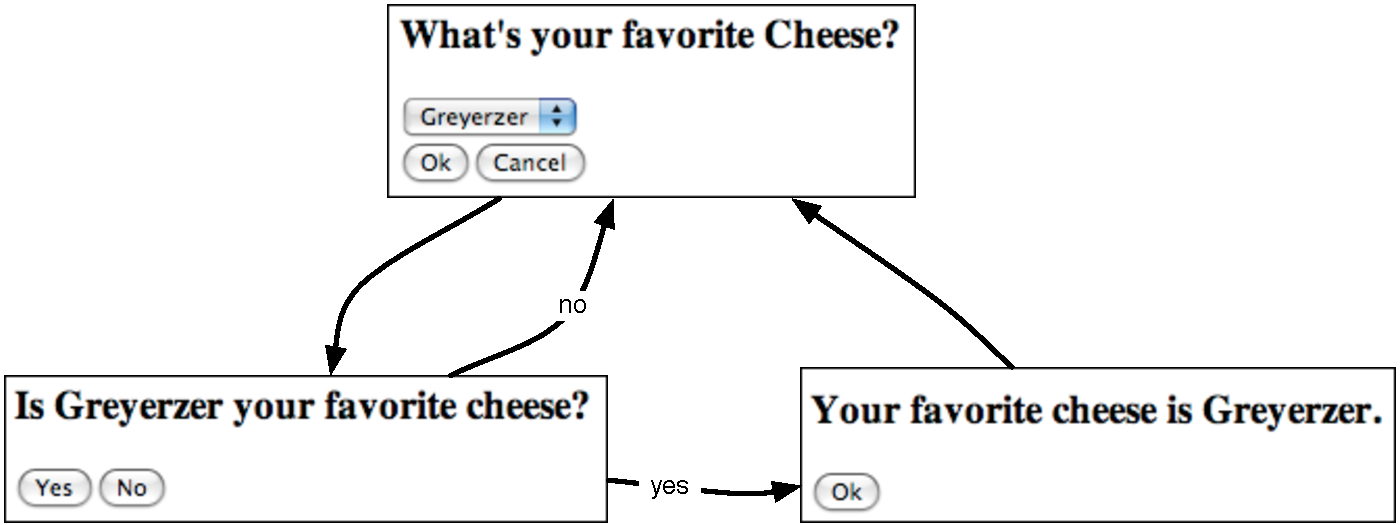
\includegraphics[width=\textwidth]{chooseCheese}
\caption{単純なタスクの例}
\figlabel{chooseCheese}
\end{center}
\end{figure}

%-----------------------------------------------------------------
\subsection{トランザクション}
% 3.0で未サポートとなった機能。訳す?

 \secref{backtracking} で Seasideはバックトラック対象となるオブジェクトを登録することで、コンポーネントの状態を、Webページごとに記録できるという話をしました。コンポーネント側でしなければならないことは、単に \ct{states} メソッドを定義して、バックトラック対象のオブジェクトを配列の形で返すだけでした。

しかし時にはバックトラックしたくないときもあります。ユーザが一度行った操作を、間違って取り消してしまうことを\emph{防ぎたい}ときがあるのです。これは「ショッピングカート問題」などと呼ばれます。ユーザがショッピングカートの精算を済ませた後は、Webブラウザのボタンで戻って、カートに商品を追加できてしまってはまずいのです。

Seasideでは\emph{トランザクション}として、いくつかの操作をひとまとめにしてタスク内で定義することによって、この機能を実現できます。
トランザクションの中ではバックトラックができますが、トランザクション終了後は戻ることができません。トランザクションを越えて戻ろうとすると、そのページは \emph{無効}になります。無効なページに戻ろうとしても、Seasideが警告を出し、直近の有効なページへと自動的にリダイレクトします。

\begin{figure}[ht]
\begin{center}
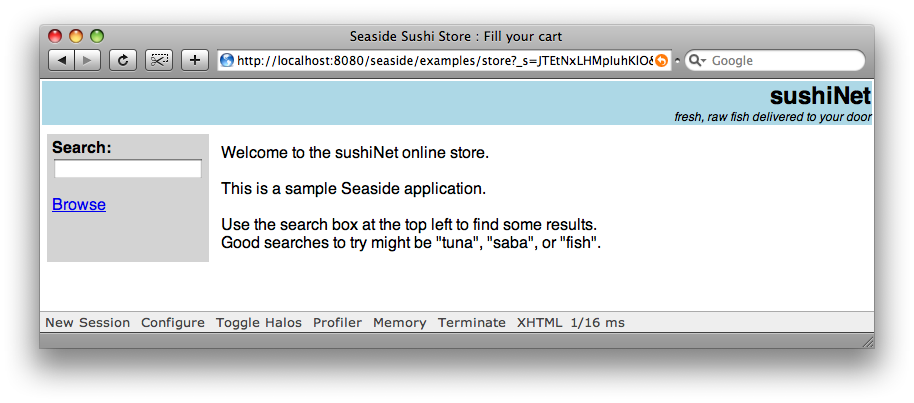
\includegraphics[width=\textwidth]{sushiStore}
\caption{寿司屋デモ}
\figlabel{sushiStore}
\end{center}
\end{figure}

Seasideの \emphsubind{Seaside}{寿司屋デモ} は、Seasideの多くの特徴を示すサンプルアプリケーションです。もちろんトランザクションも使われています。
このサンプルはSeasideに含まれており、Webブラウザで\url{http://localhost:8080/seaside/examples/store}のURLを指定すると起動します。\footnote{もしも同梱されていない場合はSqueakSourceのページ(\url{http://www.squeaksource.com/SeasideExamples/})からロードできます。 }

寿司屋デモのワークフローは以下のようになっています。
\begin{enumerate}[itemsep=0pt]
  \item サイトを訪れる
  \item 寿司をブラウズ、検索する
  \item ショッピングカートに寿司を追加する
  \item 注文処理を開始する
  \item カートの内容を確認する
  \item 届け先の住所を入力する
  \item 住所を確認する
  \item 支払い情報を入力する
  \item 寿司を待つ
\end{enumerate}

 \subind{Seaside}{ハロ}を表示させてみると、トップレベルのコンポーネントは \clsind{WAStore}となっていることがわかります。自身はタイトルバーの表示を行っているだけで、\clsind{WAStoreTask}のインスタンスである \ct{task}にレンダリングを委譲しています。

\begin{code}{}
WAStore>>>renderContentOn: html
	"... render the title bar ..."
	html div id: 'body'; with: task
\end{code}

\clsind{WAStoreTask} captures this workflow sequence. At a couple of points it is critical that the user not be able to go back and change the submitted information.

\dothis{\,``Purchase'' some sushi and then use the ``back'' button to try to put more sushi into your cart.
You will get the message ``That page has expired.''}

Seaside lets the programmer say that a certain part of a workflow act like a transaction: once the transaction is complete, the user cannot go back and undo it.
You say this by sending \mthind{WAComponent}{isolate:} to a task with the transactional block as its argument.
We can see this in the sushi store workflow as follows:

\begin{code}{}
WAStoreTask>>>go
	| shipping billing creditCard |
	cart := WAStoreCart new.
	self isolate:
		[[self fillCart.
		self confirmContentsOfCart]
			whileFalse].

	self isolate:
		[shipping := self getShippingAddress.
		billing := (self useAsBillingAddress: shipping)
					ifFalse: [self getBillingAddress]
					ifTrue: [shipping].
		creditCard := self getPaymentInfo.
		self shipTo: shipping billTo: billing payWith: creditCard].

	self displayConfirmation.
\end{code}

Here we see quite clearly that there are two transactions.
The first fills the cart and closes the shopping phase.
(The helper methods \ct{fillCart} \etc take care of instantiating and calling the right subcomponents.)
Once you have confirmed the contents of the cart you cannot go back without starting a new session.
The second transaction completes the shipping and payment data.
You can navigate back and forth within the second transaction until you confirm payment.
However, once both transactions are complete, any attempt to navigate back will fail.

Transactions may also be nested.
A simple demonstration of this is found in the class \clsind{WANestedTransaction}.
The first \ct{isolate:} takes as argument a block that contains another, nested \ct{isolate:}

\begin{code}{}
WANestedTransaction>>>go
	self inform: 'Before parent txn'.
	self isolate:
			[self inform: 'Inside parent txn'.
			self isolate: [self inform: 'Inside child txn'].
			self inform: 'Outside child txn'].
	self inform: 'Outside parent txn'
\end{code}

\dothis{Go to \url{http://localhost:8080/seaside/tests/alltests}, select \menu{WATransactionTest} and click on \button{Restart}.
Try to navigate back and forth within the parent and child transaction by clicking the \button{back} button and then clicking \button{ok}.
Note that as soon as a transaction is complete, you can no longer go back inside the transaction without generating an error upon clicking \button{ok}.}

%=================================================================
\section{A complete tutorial example}

% ON: Should take about two hours

Let's see how we can build a complete Seaside application from scratch.\footnote{The exercise should take at most a couple of hours. If you prefer to just look at the completed source code, you can grab it from the SqueakSource project \url{http://www.squeaksource.com/PharoByExample}.
The package to load is \scat{PBE-SeasideRPN}. The tutorial that follows uses slightly different class names so that you can compare your implementation with ours.}
We will build a RPN (Reverse Polish Notation) calculator as a Seaside application that uses a simple stack machine as its underlying model.
Furthermore, the Seaside interface will let us toggle between two displays\,---\,one which just shows us the current value on top of the stack, and the other which shows us the complete state of the stack.
The calculator with the two display options is shown in \figref{stackMachine}.

\begin{figure}[ht]
\begin{center}
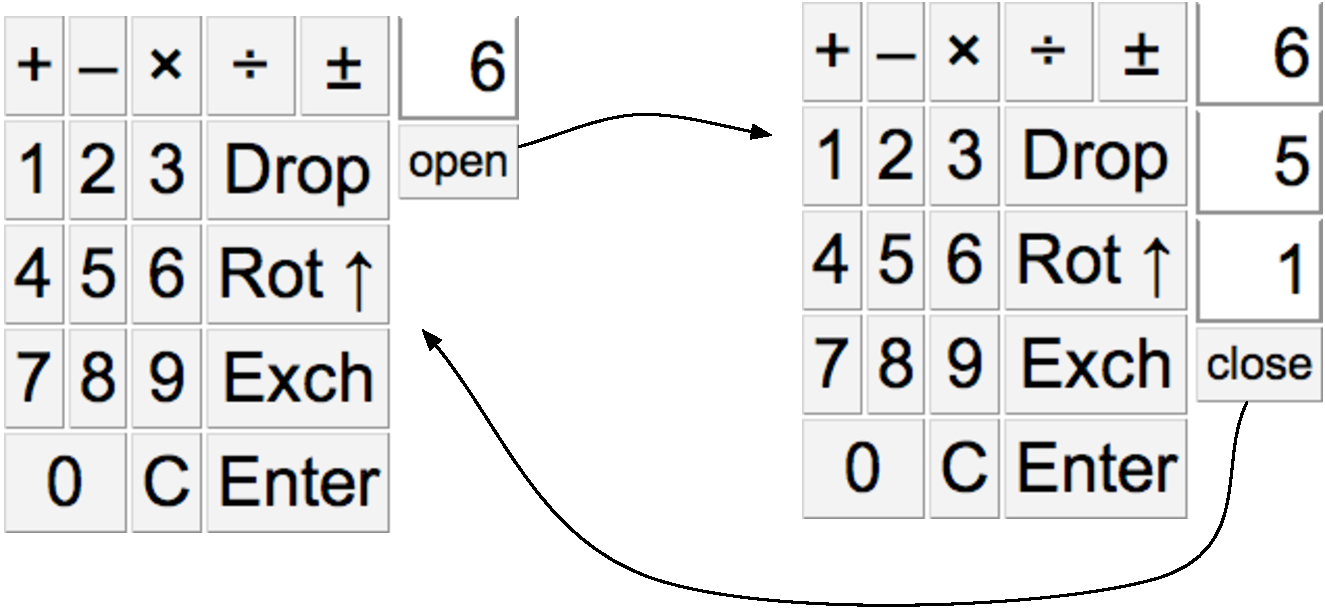
\includegraphics[width=\textwidth]{stackMachine}
\caption{RPN calculator and its stack machine}
\figlabel{stackMachine}
\end{center}
\end{figure}

We begin by implementing the stack machine and its tests.

\dothis{Define a new class called \ct{MyStackMachine} with an instance variable \ct{contents} initialized to a new \ct{OrderedCollection}.}

\begin{code}{}
MyStackMachine>>>initialize
	super initialize.
	contents := OrderedCollection new.
\end{code}

The stack machine should provide operations to \ct{push:} and \ct{pop} values, view the \ct{top} of the stack, and perform various arithmetic operations to add, subtract, multiply and divide the top values on the stack.

\dothis{Write some tests for the stack operations and then implement these operations.
Here is a sample test:}

\needlines{4}
\begin{code}{}
MyStackMachineTest>>>testDiv
	stack
		push: 3;
		push: 4;
		div.
	self assert: stack size = 1.
	self assert: stack top = (4/3).
\end{code}

You might consider using some helper methods for the arithmetic operations to check that there are two numbers on the stack before doing anything, and raising an error if this precondition is not fulfilled.\footnote{It's a good idea to use \ct{Object>>>assert:} to specify the preconditions for an operation.
This method will raise an \ct{AssertionFailure} if the user tries to use the stack machine in an invalid state.}
If you do this, most  of your methods will just be one or two lines long.

You might also consider implementing \ct{MyStackMachine>>>printOn:} to make it easier to debug your stack machine implementation with the help of an object inspector.
(Hint: just delegate printing to the \ct{contents} variable.)
\index{Object!printOn:@\ct{printOn:}}

\dothis{Complete the \ct{MyStackMachine} by writing operations \ct{dup} (push a duplicate of the top value onto the stack), \ct{exch} (exchange the top two values), and \ct{rotUp} (rotate the entire stack contents up\,---\,the top value will move to the bottom).}

Now we have a simple stack machine implementation.
We can start to implement the Seaside RPN Calculator.

We will make use of 5 classes:
\begin{itemize}
  \item \ct{MyRPNWidget}\,---\,this should be an abstract class that defines the common CSS style sheet for the application, and other common behavior for the components of the RPN calculator.
  It is a subclass of \ct{WAComponent} and the direct superclass of the following four classes. 
  
    \item \ct{MyCalculator}\,---\,this is the root component.
  It should register the application (on the class side), it should instantiate and render its subcomponents, and it should register any state for backtracking.
  \item \ct{MyKeypad}\,---\,this displays the keys that we use to interact with the calculator.
  \item \ct{MyDisplay}\,---\,this component displays the top of the stack and provides a button to call another component to display the detailed view.
  \item \ct{MyDisplayStack}\,---\,this component shows the detailed view of the stack and provides a button to answer back.
  It is a subclass of \lct{MyDisplay}.
\end{itemize}

\dothis{Define \ct{MyRPNWidget} in the category \ct{MyCalculator}.
Define the common \ct{style} for the application.}

Here is a minimal CSS for the application.
You can make it more fancy if you like.
\begin{code}{}
MyRPNWidget>>>style
	^ 'table.keypad { float: left; }
td.key {
	border: 1px solid grey;
	background: lightgrey;
	padding: 4px;
	text-align: center;
}
table.stack { float: left; }
td.stackcell {
	border: 2px solid white;
	border-left-color: grey;
	border-right-color: grey;
	border-bottom-color: grey;
	padding: 4px;
	text-align: right;
}
td.small { font-size: 8pt; }'
\end{code}

\dothis{Define \ct{MyCalculator} to be a root component and register itself as an application (\ie implement \ct{canBeRoot} and \ct{initialize} on the class side).
Implement \ct{MyCalculator>>>renderContentOn:} to render something trivial (such as its name), and verify that the application runs in a browser.
}

\ct{MyCalculator} is responsible for instantiating \ct{MyStackMachine}, \ct{MyKeypad} and \ct{MyDisplay}.

\dothis{
Define \ct{MyKeypad} and \ct{MyDisplay} as subclasses of \lct{MyRPNWidget}.
All three components will need access to a common instance of the stack machine, so define the instance variable \ct{stackMachine} and an initialization method \ct{setMyStackMachine:} in the common parent, \ct{MyRPNWidget}.
Add instance variables \ct{keypad} and \ct{display} to \ct{MyCalculator} and initialize them in \ct{MyCalculator>>>initialize}.
(Don't forget to send \lct{super initialize}!)}

\dothis{
Pass the shared instance of the stack machine to the keypad and the display in the same initialize method.
Implement \ct{MyCalculator>>>renderContentOn:} to simply render in turn the keypad and the display.
To correctly display the subcomponents, you must implement \ct{MyCalculator>>>children} to return an array with the keypad and the display.
Implement placeholder rendering methods for the keypad and the display and verify that the calculator now displays its two subcomponents.
}

%\ab{Too long!}

Now we will change the implementation of the display to show the top value of the stack.

\dothis{
Use a table with class ``keypad'' containing a row with a single table data cell with class ``stackcell''.
Change the rendering method of the keypad to ensure that the number 0 is pushed on the stack in case it is empty.
(Define and use \ct{MyKeypad>>>ensureMyStackMachineNotEmpty}.)
Also make it display an empty table with class ``keypad''.
Now the calculator should display a single cell containing the value 0.
If you toggle the halos, you should see something like this:
}

\begin{figure}[ht]
\begin{center}
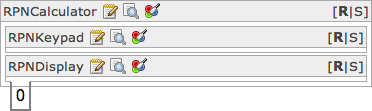
\includegraphics[width=0.8\textwidth]{firstStackDisplay}
\caption{Displaying the top of the stack}
\figlabel{firstStackDisplay}
\end{center}
\end{figure}

Now let's implement an interface to interact with the stack.

\dothis{
First define the following helper methods, which will make it easier to script the interface:
}

\needlines{3}
\begin{code}{}
MyKeypad>>>renderStackButton: text callback: aBlock colSpan: anInteger on: html 
	html tableData
		class: 'key';
		colSpan: anInteger;
		with: 
				[html anchor
					callback: aBlock;
					with: [html html: text]]
\end{code}


\begin{code}{}
MyKeypad>>>renderStackButton: text callback: aBlock on: html 
	self 
		renderStackButton: text
		callback: aBlock
		colSpan: 1
		on: html
\end{code}

We will use these two methods to define the buttons on the keypad with appropriate callbacks.
Certain buttons may span multiple columns, but the default is to occupy just one column.

\dothis{
Use the two helper methods to script the keypad as follows:
(Hint: start by getting the digit and ``Enter'' keys working, then the arithmetic operators.)
}

\needlines{4}
\begin{code}{}
MyKeypad>>>renderContentOn: html 
  self ensureStackMachineNotEmpty.
  html table
    class: 'keypad';
    with: [
      html tableRow: [
          self renderStackButton: '+' callback: [self stackOp: #add] on: html.
          self renderStackButton: '&ndash;' callback: [self stackOp: #min] on: html.
          self renderStackButton: '&times;' callback: [self stackOp: #mul] on: html.
          self renderStackButton: '&divide;' callback: [self stackOp: #div] on: html.
          self renderStackButton: '&plusmn;' callback: [self stackOp: #neg] on: html ].
        html tableRow: [
          self renderStackButton: '1' callback: [self type: '1'] on: html.
          self renderStackButton: '2' callback: [self type: '2'] on: html.
          self renderStackButton: '3' callback: [self type: '3'] on: html.
          self renderStackButton: 'Drop' callback: [self stackOp: #pop]
          	colSpan: 2 on: html ].
" and so on ... "
        html tableRow: [
          self renderStackButton: '0' callback: [self type: '0'] colSpan: 2 on: html.
          self renderStackButton: 'C' callback: [self stackClearTop] on: html.
          self renderStackButton: 'Enter'
          	callback: [self stackOp: #dup. self setClearMode]
			colSpan: 2 on: html ]]
\end{code}

Check that the keypad displays properly.
If you try to click on the keys, however, you will find that the calculator does not work yet\ldots{}

\dothis{
Implement \ct{MyKeypad>>>type:} to update the top of the stack by appending the typed digit.
You will need to convert the top value to a string, update it, and convert it back to an integer, something like this:
}
\begin{code}{}
MyKeypad>>>type: aString
	stackMachine push: (stackMachine pop asString, aString) asNumber.
\end{code}
Now when you click on the digit keys the display should be updated.
(Be sure that \ct{MyStackMachine>>>pop} returns the value popped, or this will not work!)


\dothis{Now we must implement \ct{MyKeypad>>>stackOp:}
Something like this will do the trick:}

\begin{code}{}
MyKeypad>>>stackOp: op
	[ stackMachine perform: op ] on: AssertionFailure do: [ ].
\end{code}

The point is that we are not sure that all operations will succeed, for example, addition will fail if we do not have two numbers on the stack.
For the moment we can just ignore such errors.
If we are feeling more ambitious later on, we can provide some user feedback in the error handler block.

\dothis{The first version of the calculator should be working now.
Try to enter some numbers by pressing the digit keys, hitting \menu{Enter} to push a copy of the current value, and entering \menu{+} to sum the top two values.}

You will notice that typing digits does not behave the way you might expect.
Actually the calculator should be aware of whether you are typing a \emph{new} number, or appending to an existing number.

\dothis{Adapt \ct{MyKeypad>>>type:} to behave differently depending on the current typing mode.
Introduce an instance variable \ct{mode} which takes on one of the three values \lct{\#typing} (when you are typing), \lct{\#push} (after you have performed a calculator operation and typing should force the top value to be pushed), or \lct{\#clear} (after you have performed \menu{Enter} and the top value should be cleared before typing).
The new \ct{type:} method might look like this:
}

\begin{code}{}
MyKeypad>>>type: aString
	self inPushMode ifTrue: [
		stackMachine push: stackMachine top.
		self stackClearTop ].
	self inClearMode ifTrue: [ self stackClearTop ].
	stackMachine push: (stackMachine pop asString, aString) asNumber.
\end{code}
\mb{better with "stackMachine dup" instead of "stackMachine push:
  stackMachine top}"

Typing might work better now, but it is still frustrating not to be able to see what is on the stack.

\dothis{
Define \ct{MyDisplayStack} as a subclass of \ct{MyDisplay}.
Add a button to the rendering method of \ct{MyDisplay} which will call a new instance of \ct{MyDisplayStack}.
You will need an html anchor that looks something like this:
}

\begin{code}{}
html anchor
	callback: [ self call: (MyDisplayStack new setMyStackMachine: stackMachine)];
	with: 'open'
\end{code}
\mb{if the user got a stackmachine ivar, I'm sure he will define
  setStackMachine and not setMyStackMachine}


The callback will cause the current instance of \ct{MyDisplay} to be temporarily replaced by a new instance of \ct{MyDisplayStack} whose job it is to display the complete stack.
When this component signals that it is done (\ie by sending \ct{self answer}), then control will return to the original instance of \ct{MyDisplay}.

\dothis{
Define the rendering method of \ct{MyDisplayStack} to display all of the values on the stack.
(You will either need to define an accessor for the stack machine's \ct{contents} or you can define \ct{MyStackMachine>>>do:} to iterate over the stack values.)
The stack display should also have a button labelled ``close'' whose callback will simply perform \ct{self answer}.
}

\begin{code}{}
html anchor
	callback: [ self answer];
	with: 'close'
\end{code}

Now you should be able to \emph{open} and \emph{close} the stack while you are using the calculator.

There is, however, one thing we have forgotten.
Try to perform some operations on the stack.
Now use the ``back'' button of your browser and try to perform some more stack operations.
(For example, \menu{open} the stack, type \menu{1}, \menu{Enter} twice and \menu {+}.
The stack should display ``2'' and ``1''.
Now hit the ``back'' button.
The stack now shows three times ``1'' again.
Now if you type \menu{+} the stack shows ``3''.
Backtracking is not yet working.

\dothis{
Implement \ct{MyCalculator>>>states} to return 
an array with the contents of the stack machine.
Check that backtracking now works correctly!
}

Sit back and enjoy a tall glass of something cool!

%=================================================================
\section{A quick look at AJAX}

% Original text by Lukas Renggli

\ind{AJAX} (Asynchronous \ind{JavaScript} and \ind{XML}) is a technique to make web applications more interactive by exploiting JavaScript functionality on the client side.

Two well-known JavaScript libraries are \ind{Prototype} (\url{http://www.prototypejs.org}) and \ind{script.aculo.us} (\url{http://script.aculo.us}).
Prototype provides a framework to ease writing JavaScript.
script.aculo.us provides some additional features to support animations and drag-and-drop on top of Prototype.
Both frameworks are supported in Seaside through the package ``Scriptaculous''.

All ready-made images have the Scriptaculous package extensions already loaded.
The latest version is available from \url{http://www.squeaksource.com/Seaside}.
An online demo is available at \url{http://scriptaculous.seasidehosting.st}.
Alternatively, if you have a enabled image running, simply go to \url{http://localhost:8080/seaside/tests/scriptaculous}.

The Scriptaculous extensions follow the same approach as Seaside itself\,---\,simply configure Smalltalk objects to model your application, and the needed Javascript code will be generated for you.

Let us look at a simple example of how client-side Javascript support can make our RPN calculator behave more naturally.
Currently every keystroke to enter a digit generates a request to refresh the page.
We would like instead to handle editing of the display on the client-side by updating the display in the existing page.

\dothis{To address the display from JavaScript code we must first give it a unique id.
Update the calculator's rendering method as follows:\footnote{If you have not implemented the tutorial example yourself, you can simply load the complete example (PBE-SeasideRPN) from \url{http://www.squeaksource.com/PharoByExample} and apply the suggested changes to the classes \ct{RPN*} instead of \ct{My*}.}}

\begin{code}{}
MyCalculator>>>renderContentOn: html
	html div id: 'keypad'; with: keypad.
	html div id: 'display'; with: display.	
\end{code}

\mb{'keyboard' below should be renamed 'keypad'}
\dothis{To be able to re-render the display when a keyboard button is pressed, the keyboard needs to know the display component.
Add a \ct{display} instance variable to \ct{MyKeypad}, an initialize method \ct{MyKeypad>>>setDisplay:}, and call this from \ct{MyCalculator>>initialize}.
Now we are able to assign some JavaScript code to the buttons by updating \ct{MyKeypad>>>renderStackButton:callback:colSpan:on:} as follows:}

\begin{code}{}
MyKeypad>>>renderStackButton: text callback: aBlock colSpan: anInteger on: html 
	html tableData
		class: 'key';
		colSpan: anInteger;
		with: [
			html anchor
				callback: aBlock;
				onClick:				"handle Javascript event"
					(html updater
						id: 'display';
						callback: [ :r |
							aBlock value.
							r render: display ];
						return: false);
				with: [ html html: text ] ]
\end{code}

\mthind{WATagBrush}{onClick:} specifies a \ind{JavaScript} event handler.
\ct{html updater} returns an instance of \ct{SUUpdater}, a Smalltalk object representing the JavaScript Ajax.Updater object (\url{http://www.prototypejs.org/api/ajax/updater}).
This object performs an AJAX request and updates a container's contents based on the response text.
\ct{id:} tells the updater what XHTML DOM element to update, in this case the contents of the div element with the id 'display'.
\ct{callback:} specifies a block that is triggered when the user presses the button.
The block argument is a new renderer \ct{r}, which we can use to render the display component.
(Note: Even though html is still accessible, it is not valid anymore at the time this callback block is evaluated).
Before rendering the display component we evaluate \ct{aBlock} to perform the desired action.

\ct{return: false} tells the JavaScript engine to not trigger the original link callback, which would cause a full refresh.
We could instead remove the original anchor \ct{callback:}, but like this the calculator will still work even if JavaScript is disabled.

\dothis{Try the calculator again, and notice how a full page refresh is triggered every time you press a digit key. (The URL of the web page is updated at each keystroke.)}

Although we have implemented the client-side behavior, we have not yet activated it.
Now we will enable the Javascript event handling.

\dothis{
Click on the \link{Configure} link in the toolbar of the calculator.
Select ``Add Library:'' \ct{SULibrary}, click the \button{Add} button and \button{Close}.}

Instead of manually adding the library, you may also do it programmatically when you register the application:
\begin{code}{}
MyCalculator class>>>initialize
	(self registerAsApplication: 'rpn')
		addLibrary: SULibrary
\end{code}

\begin{figure}[ht]
\begin{center}
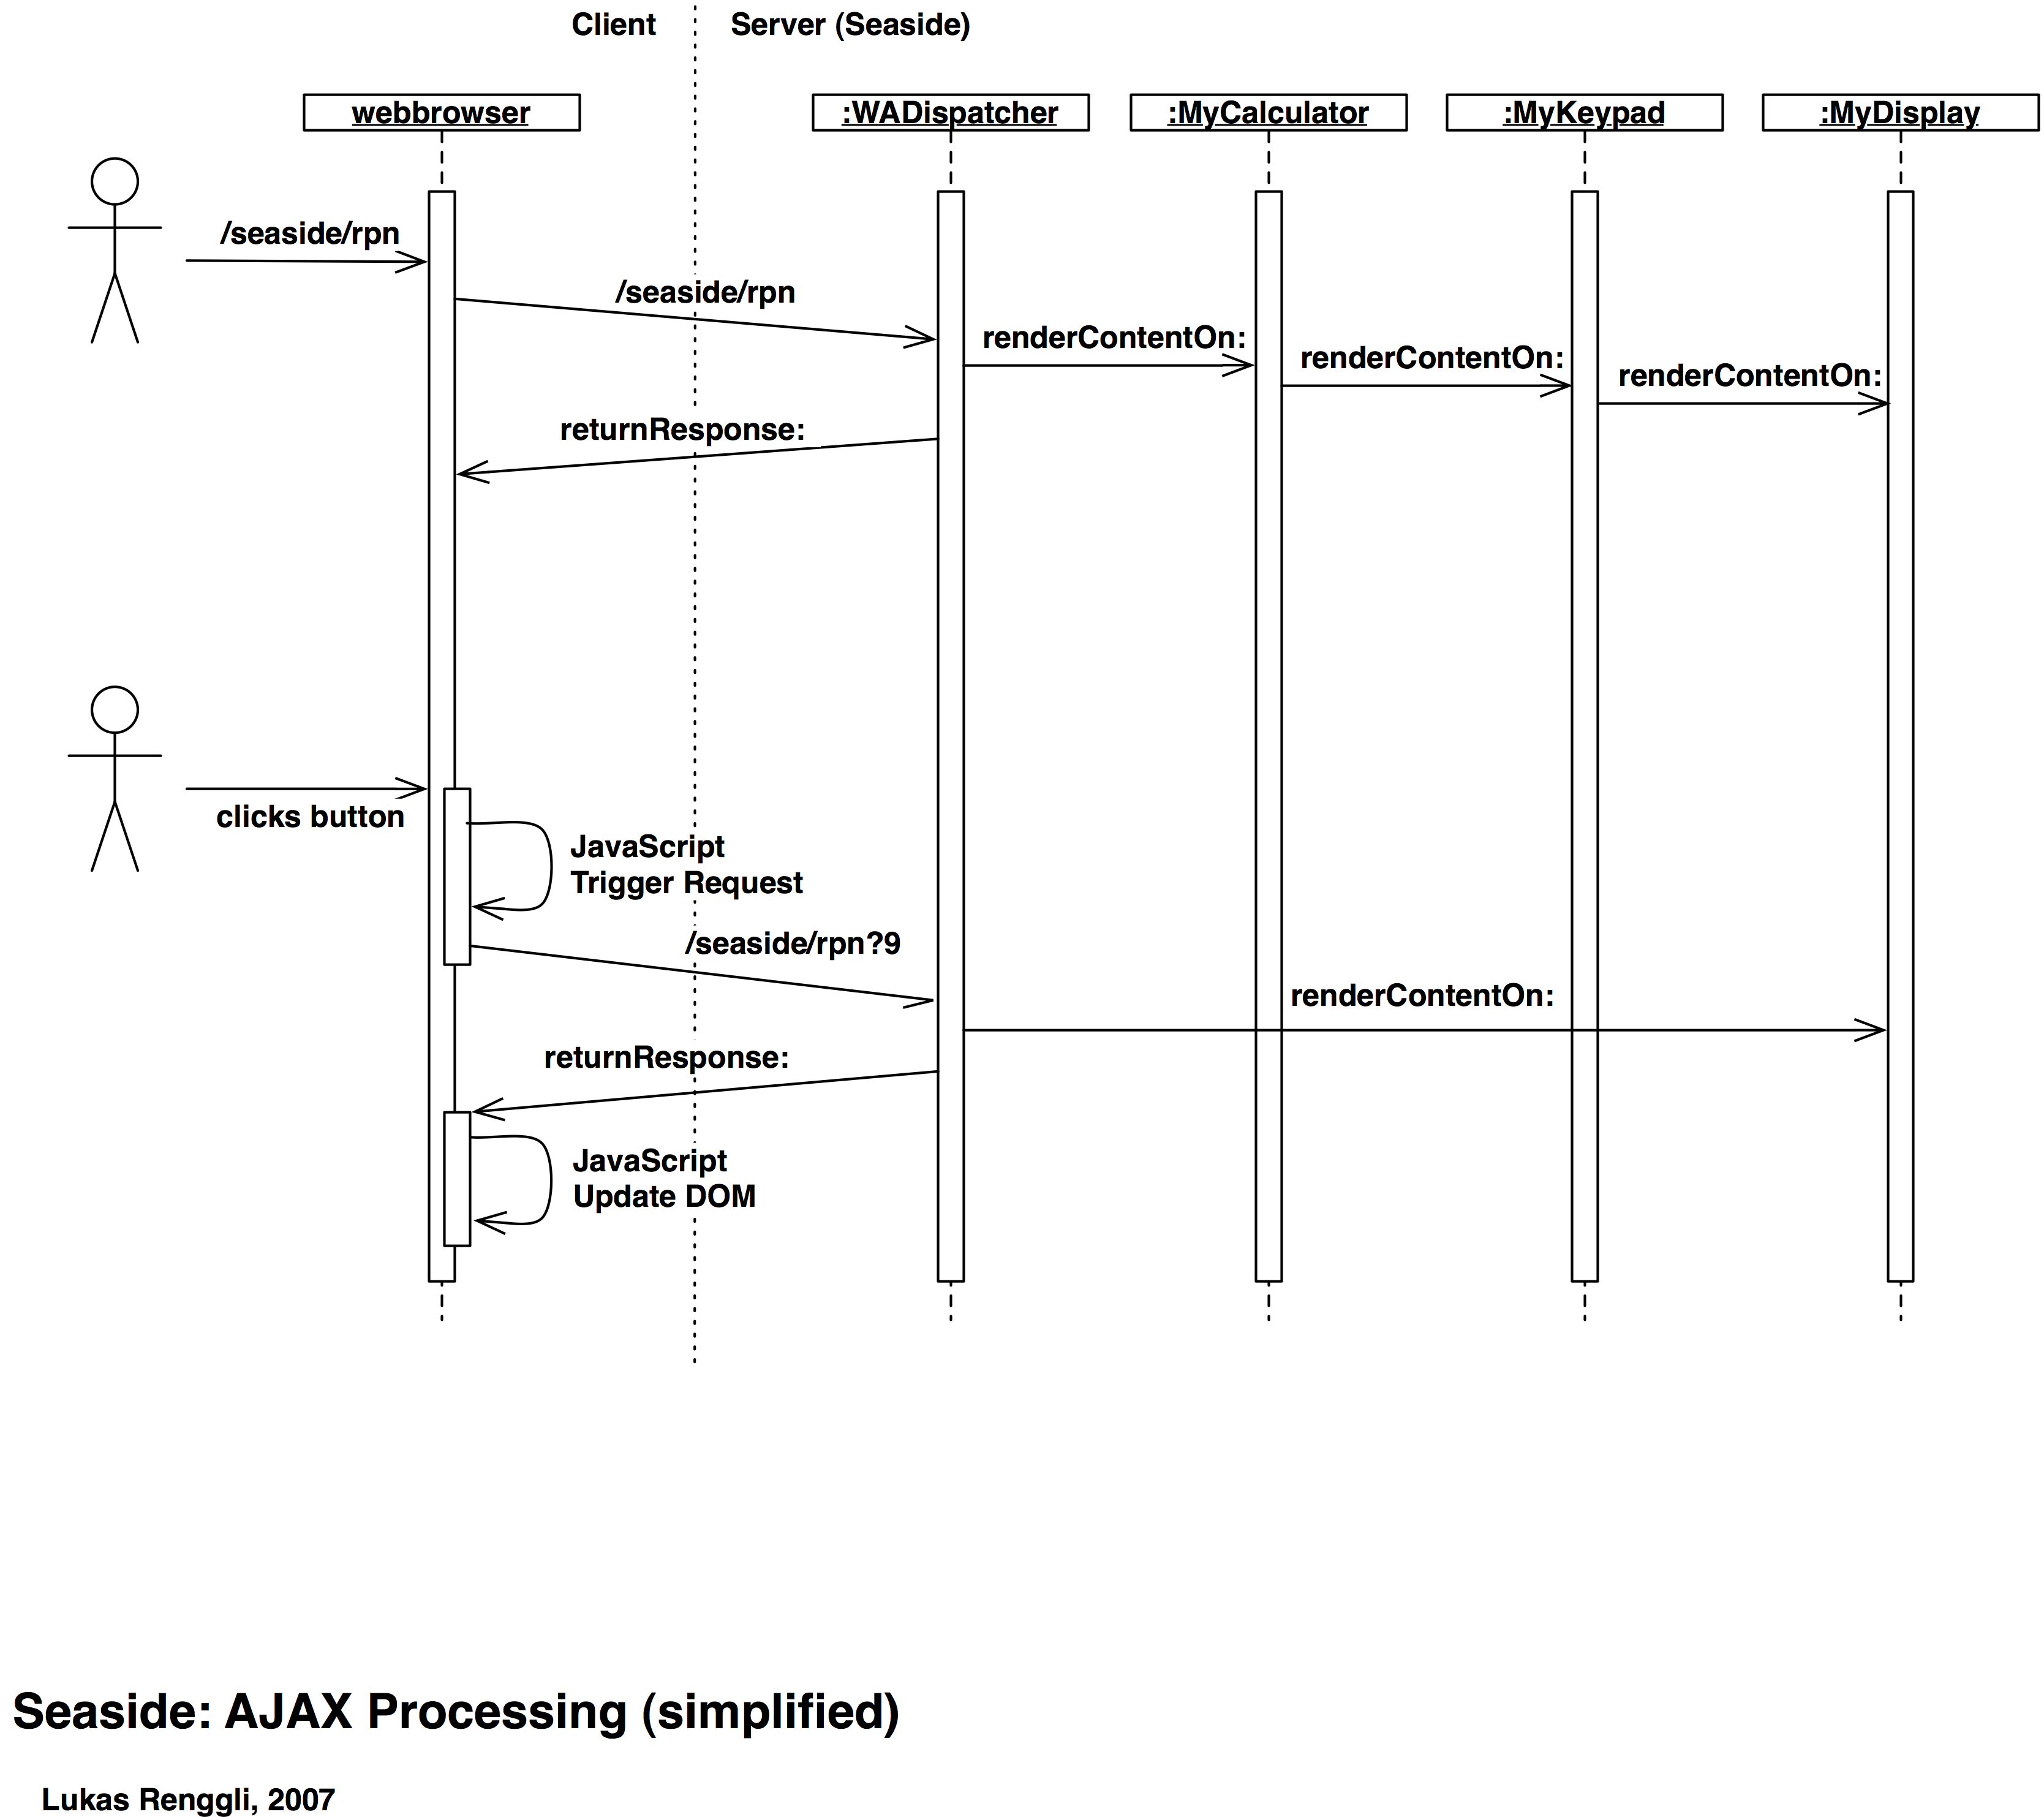
\includegraphics[width=\textwidth]{ajax-processing}
\caption{Seaside AJAX processing (simplified)}
\figlabel{ajax-processing}
\end{center}
\end{figure}

\dothis{Try the revised application.  Note that the feedback is much more natural. In particular, a new URL is not generated with each keystroke.}

You may well ask, \emph{yes, but how does this work?}
\figref{ajax-processing} shows how the RPN applications would both without and with AJAX.
Basically AJAX short-circuits the rendering to \emph{only} update the display component.
Javascript is responsible both for triggering the request and updating the corresponding DOM element.
Have a look at the generated source-code, especially the JavaScript code:

\begin{code}{}
new Ajax.Updater(
	'display',
	'http://localhost/seaside/RPN+Calculator',
	{'evalScripts': true,
	  'parameters': ['UNDERSCOREs=zcdqfonqwbeYzkza', 'UNDERSCOREk=jMORHtqr','9'].join('&')});
return false
\end{code}

For more advanced examples, have a further look at \url{http://localhost:8080/seaside/tests/scriptaculous}.

\paragraph{\emph{Hints.}}
In case of server side problems use the Smalltalk debugger.
In case of client side problems use FireFox (\url{http://www.mozilla.com}) with the JavaScript debugger FireBug (\url{http://www.getfirebug.com/}) plugin enabled.

%=================================================================
\section{Chapter summary}

\begin{itemize}
  \item The easiest way to get started is to download the ``Seaside One-Click Experience'' from \url{http://seaside.st}
  \item Turn the server on and off by evaluating \ct{WAKom startOn: 8080} and \ct{WAKom stop}.
  \item Reset the administrator login and password by evaluating \ct{WADispatcherEditor initialize}.
  \item \menu{Toggle Halos} to directly view application source code, run-time objects, CSS and XHTML.
  \item Send \ct{WAGlobalConfiguration setDeploymentMode} to hide the toolbar.
  \item Seaside web applications are composed of components, each of which is an instance of a subclass of \ct{WAComponent}.
  \item Only a root component may be registered as an application. It should implement \ct{canBeRoot} on the class side. Alternatively it may register itself as an application in its class-side \ct{initialize} method by sending \ct{self registerAsApplication:} \emph{application path}.
  If you override \ct{description} it is possible to return a descriptive application name that will be displayed in the configuration editor.
  \mb{the description thing is not mentionned anywhere}
  \item To backtrack state, a component must implement the \ct{states} method to answer an array of objects whose state will be restored if the user clicks the browser's ``back'' button.
  \item A component renders itself by implementing \ct{renderContentOn:}.
  The argument to this method is an XHTML rendering \emph{canvas} (usually called \ct{html}).
  \item A component can render a subcomponent by sending \ct{self render:} \emph{subcomponent}.
  \item XHTML is generated programmatically by sending messages to \emph{brushes}. A brush is obtained by sending a message, such as \ct{paragraph} or \ct{div}, to the html canvas.
  \item If you send a cascade of messages to a brush that includes the message \ct{with:}, then \ct{with:} should be the last message sent.
  The \ct{with:} message sets the contents \emph{and} renders the result.
  \item Actions should appear only in callbacks.
You should not change the state of the application while you are rendering it.
  \item You can bind various form widgets and anchors to instance variables with accessors by sending the message \ct{on:} \emph{instance variable} \ct{of:} \emph{object} to the brush.
  \item You can define the CSS for a component hierarchy by defining the method \ct{style}, which should return a string containing the style sheet.
  (For deployed applications, it is more usual to refer to a style sheet located at a static URL.)
  \item Control flows can be programmed by sending \ct{x call: y}, in which case component \ct{x} will be replaced by \ct{y} until \ct{y} answers by sending \ct{answer:} with a result in a callback.
  The receiver of \ct{call:} is usually \ct{self}, but may in general be any visible component.
  \item A control flow can also be specified as a \emph{task}\,---\,a instance of a subclass of \ct{WATask}. It should implement the method \ct{go}, which should \ct{call:} a series of components in a workflow.
  \item Use \ct{WAComponents}'s convenience methods \ct{request:}, \ct{inform:}, \ct{confirm:} and \ct{chooseFrom:caption:} for basic interactions.
  \item To prevent the user from using the browser's ``back'' button to access a previous execution state of the web application, you can declare portions of the workflow to be a \emph{transaction} by enclosing them in an \ct{isolate:} block.
\end{itemize}
%-----------------------------------------------------------------

%=================================================================
\ifx\wholebook\relax\else 
   \bibliographystyle{jurabib}
   \nobibliography{scg}
   \end{document}
\fi
%=================================================================
